\chapter{Appendix}
\thesisspacing

% ============================================================
%  Render and hardware image gallery.
%  Layout: 2 columns x 3 rows per page, vfill to fill height.
%  All AppendixA/ images live in imgs/AppendixA/ on Overleaf.
% ============================================================

% ----------------------------------------------------------------
%  Page 1 — Early stereo renders: debug, gyroid, torus, hyperboloid,
%            scaffold lattice, gyroid spheres
% ----------------------------------------------------------------
\begin{figure}[H]
\vspace*{-0.5cm}
\centering
\begin{subfigure}[b]{0.48\textwidth}
    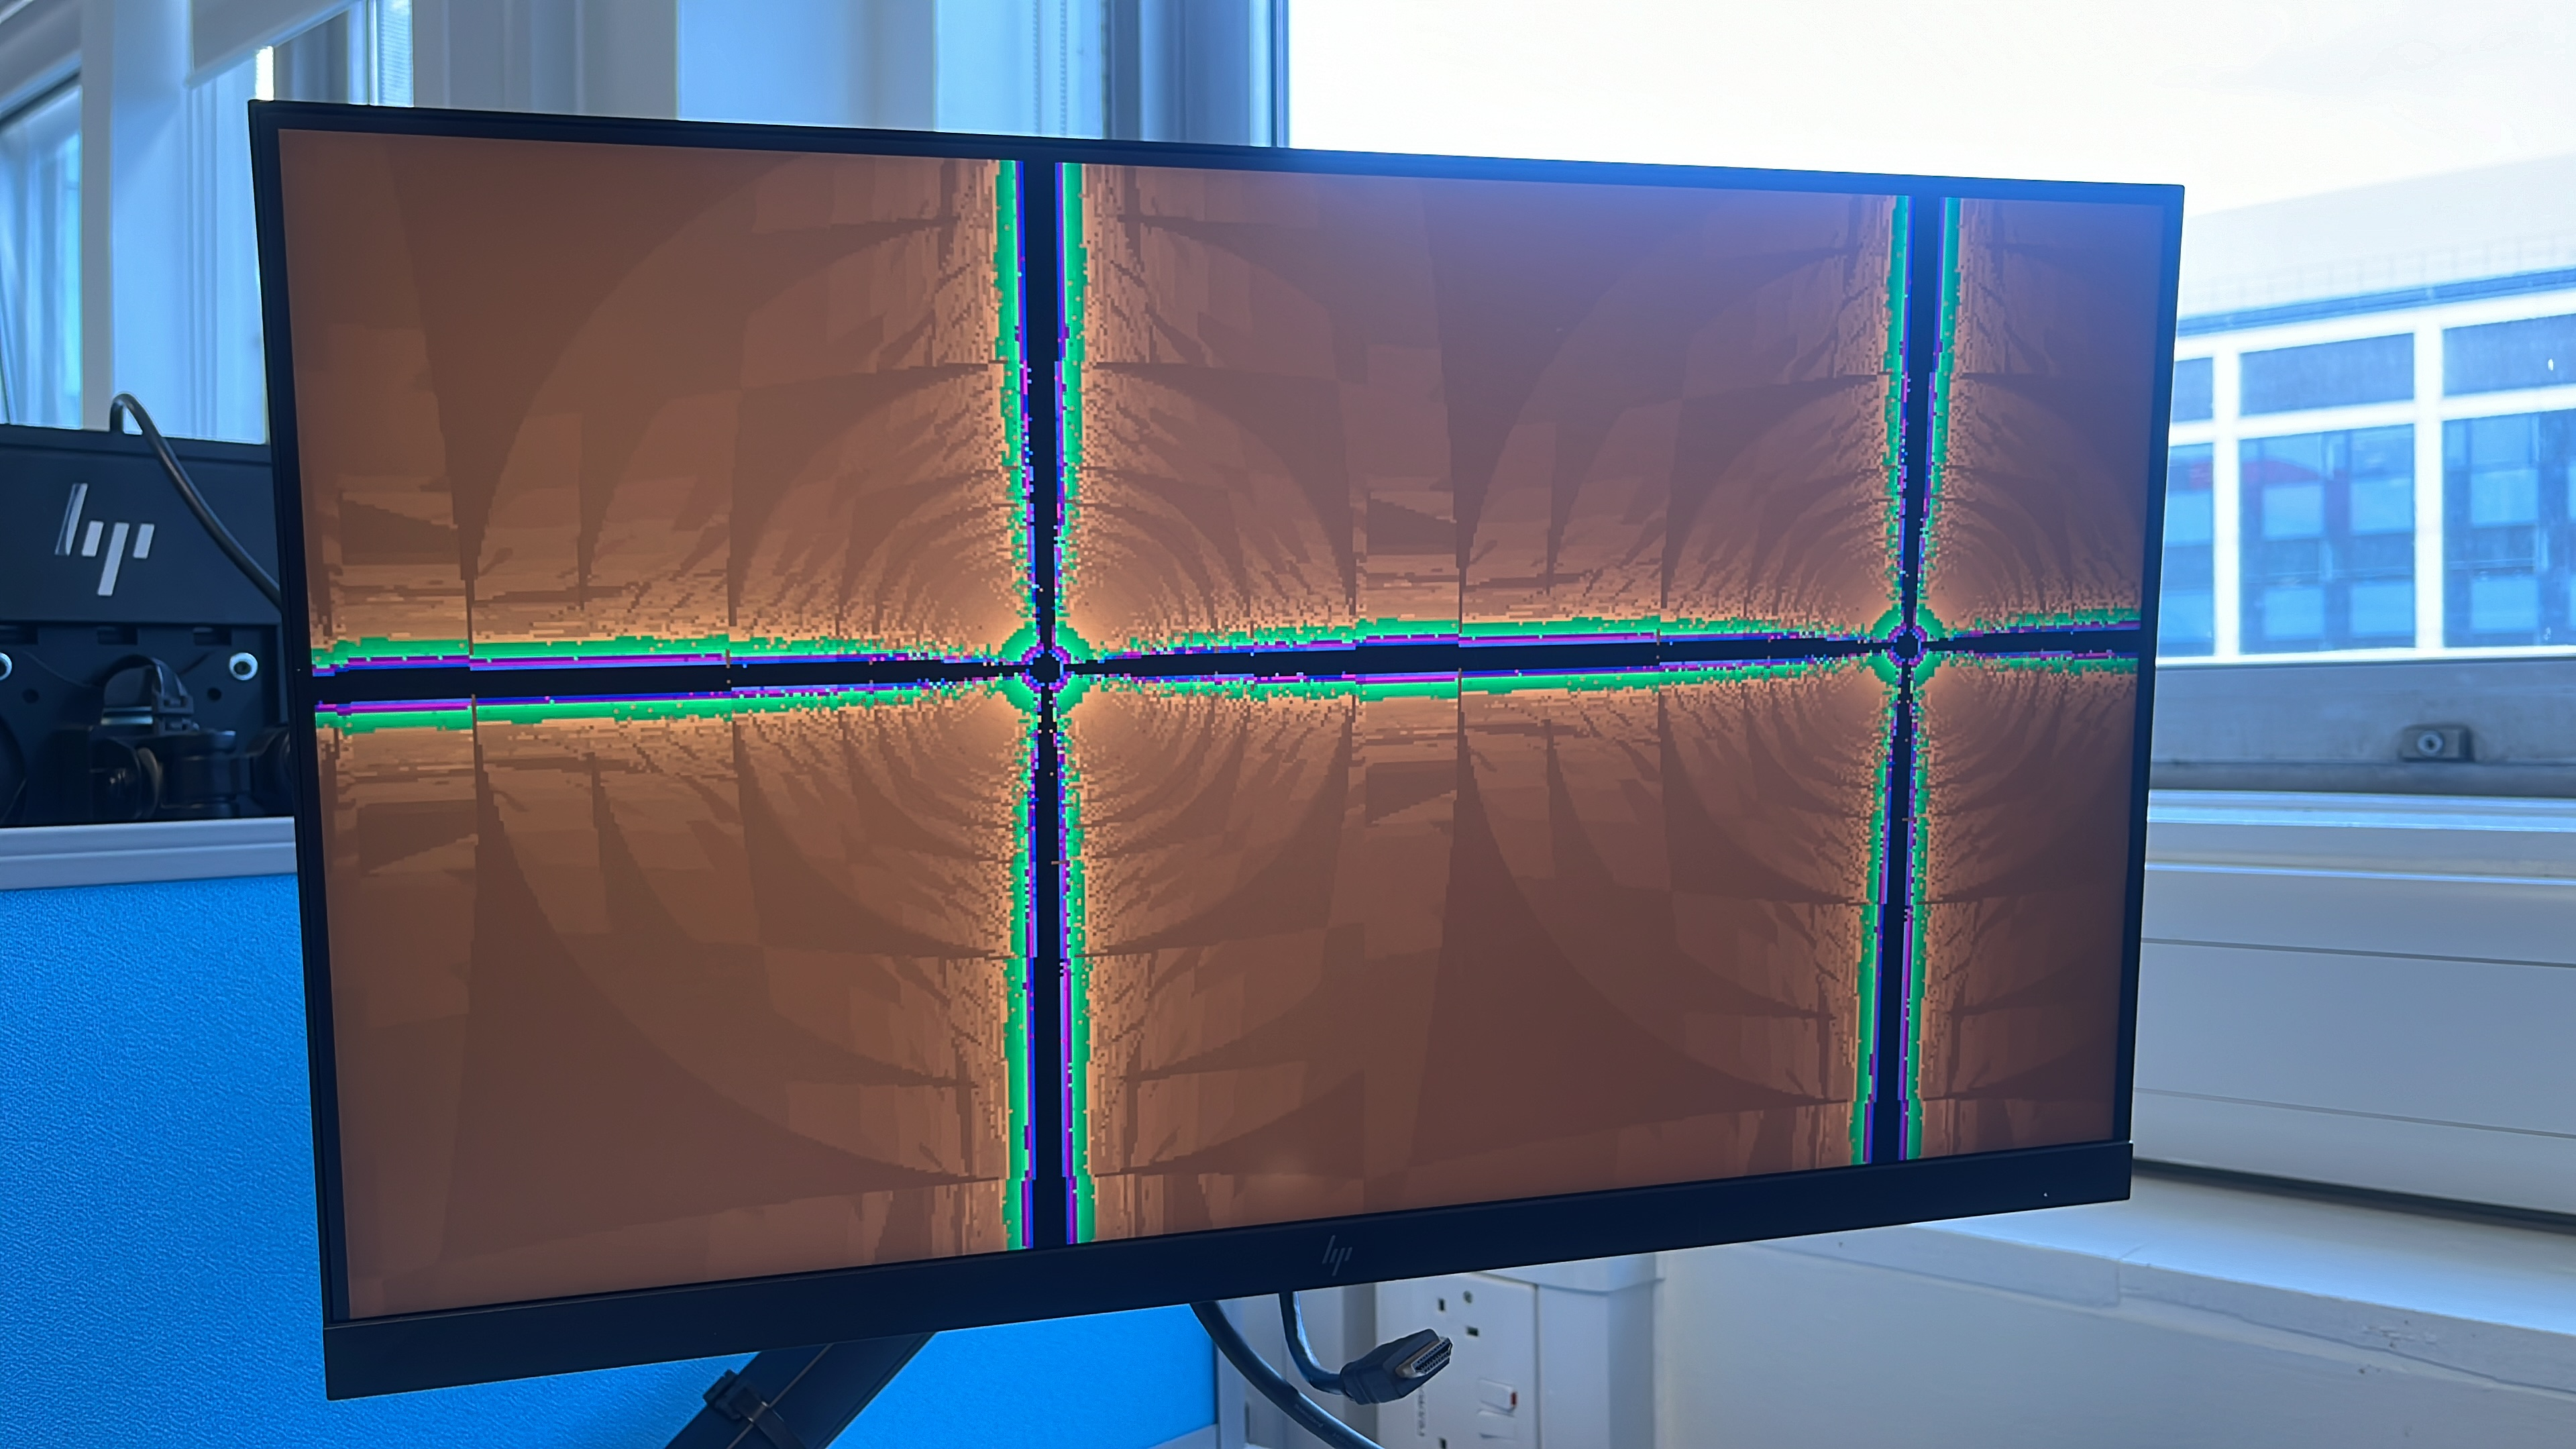
\includegraphics[width=\textwidth,height=0.28\textheight,keepaspectratio]{imgs/AppendixA/render_scaffold_debug_early.jpg}
    \caption{Early mandelbox debug render. Orange cross-hatch output; sync artefacts visible from uncalibrated VDMA buffer timing.}
\end{subfigure}\hfill
\begin{subfigure}[b]{0.48\textwidth}
    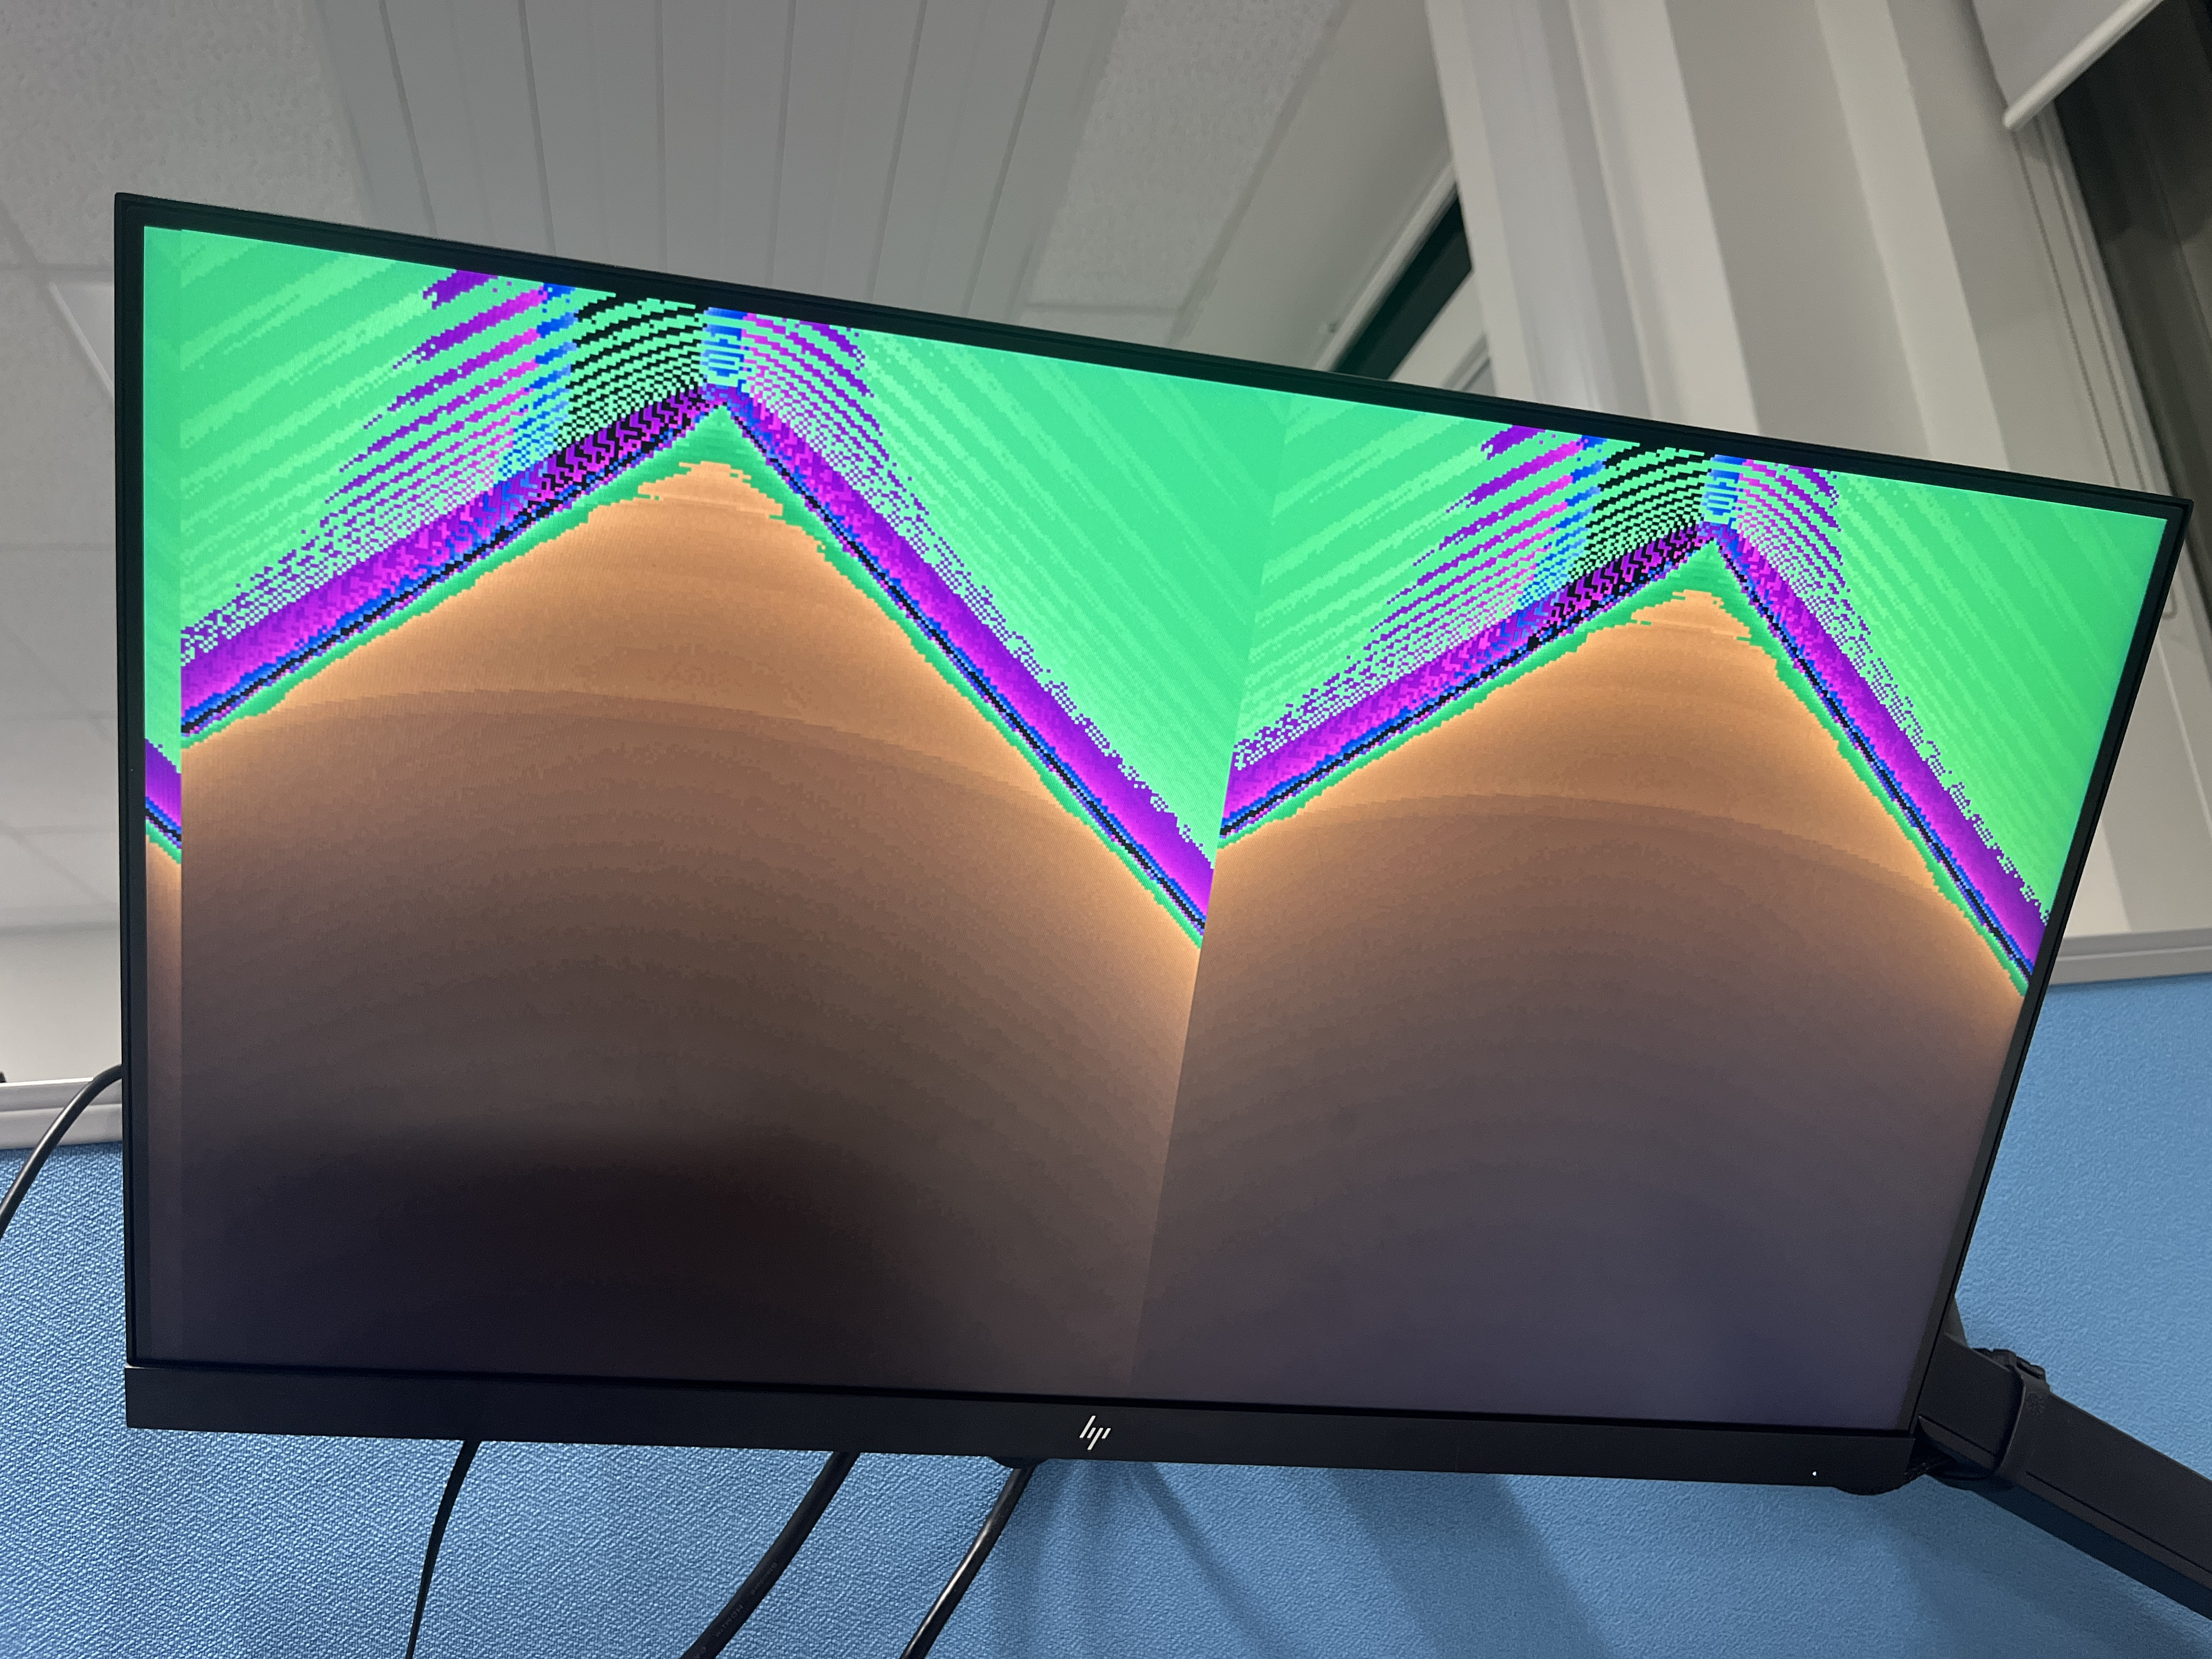
\includegraphics[width=\textwidth,height=0.28\textheight,keepaspectratio]{imgs/AppendixA/render_gyroid_early_stereo.jpg}
    \caption{Early cone, stereoscopic output. Wavy organic geometry with green--purple--orange iteration palette.}
\end{subfigure}

\vfill

\begin{subfigure}[b]{0.48\textwidth}
    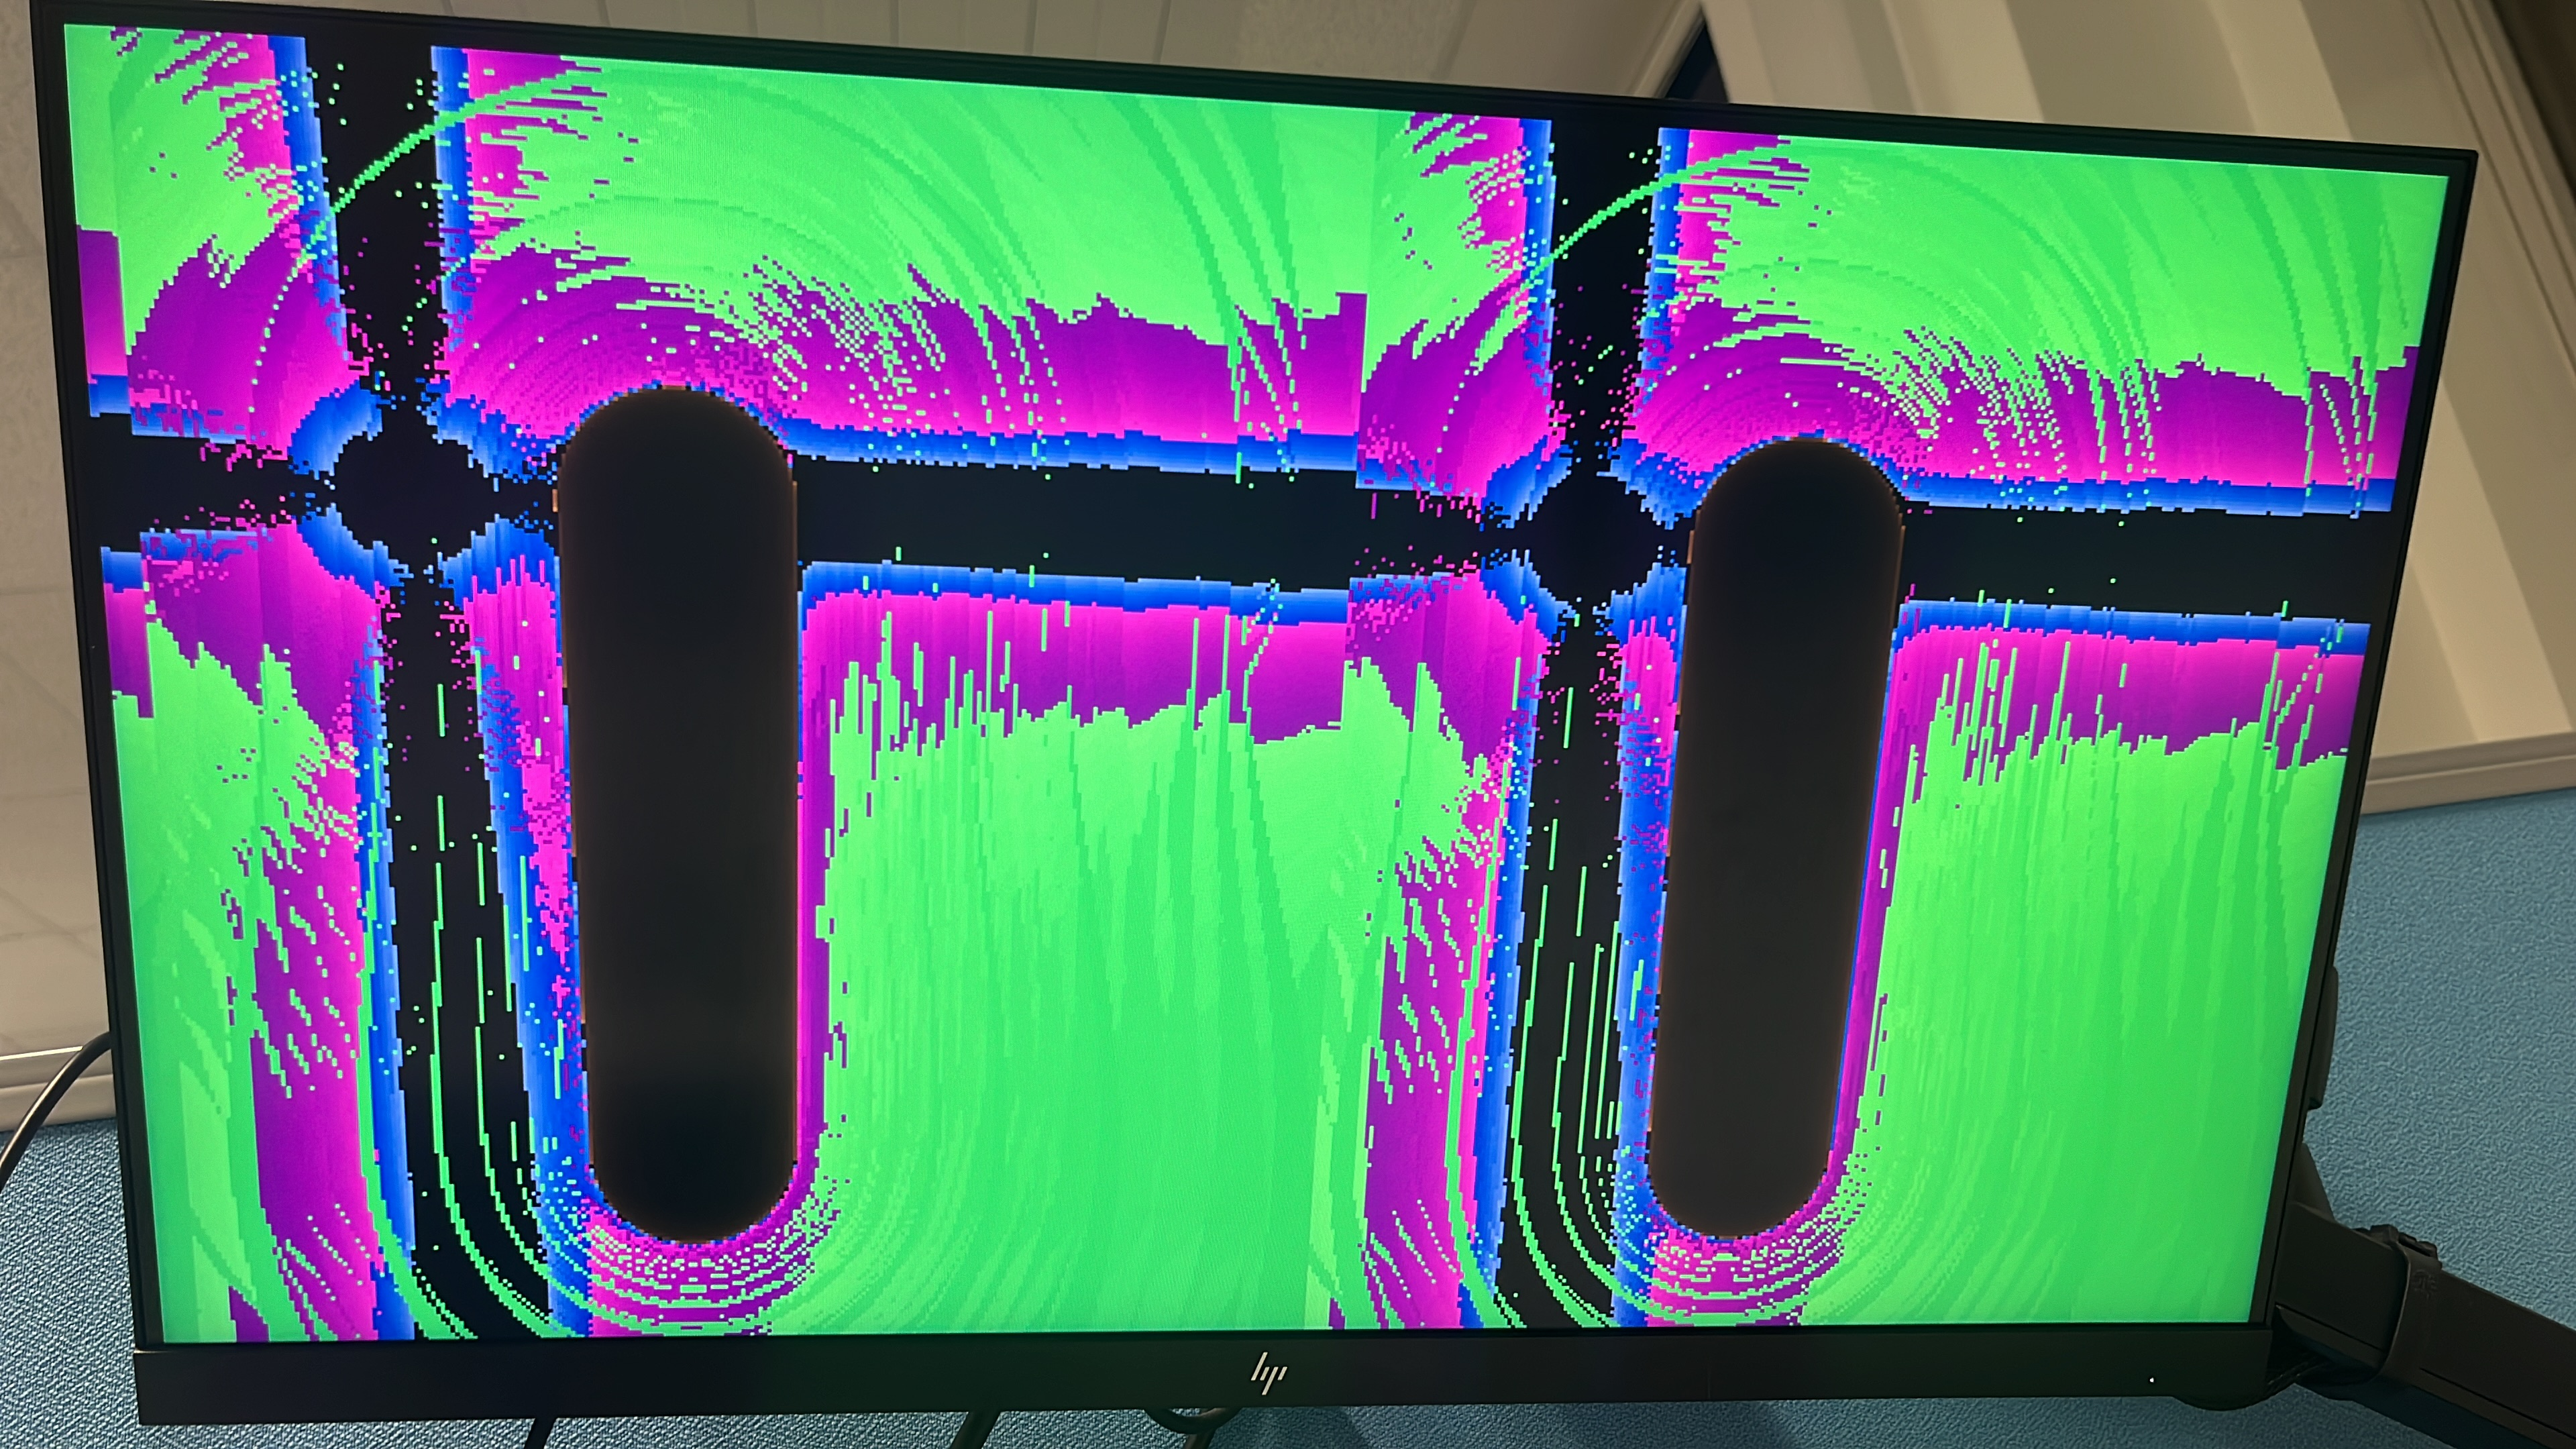
\includegraphics[width=\textwidth,height=0.28\textheight,keepaspectratio]{imgs/AppendixA/render_torus_stereo.jpg}
    \caption{Torus SDF in stereoscopic mode. Vivid green--purple colourmap; concave annular region visible at centre.}
\end{subfigure}\hfill
\begin{subfigure}[b]{0.48\textwidth}
    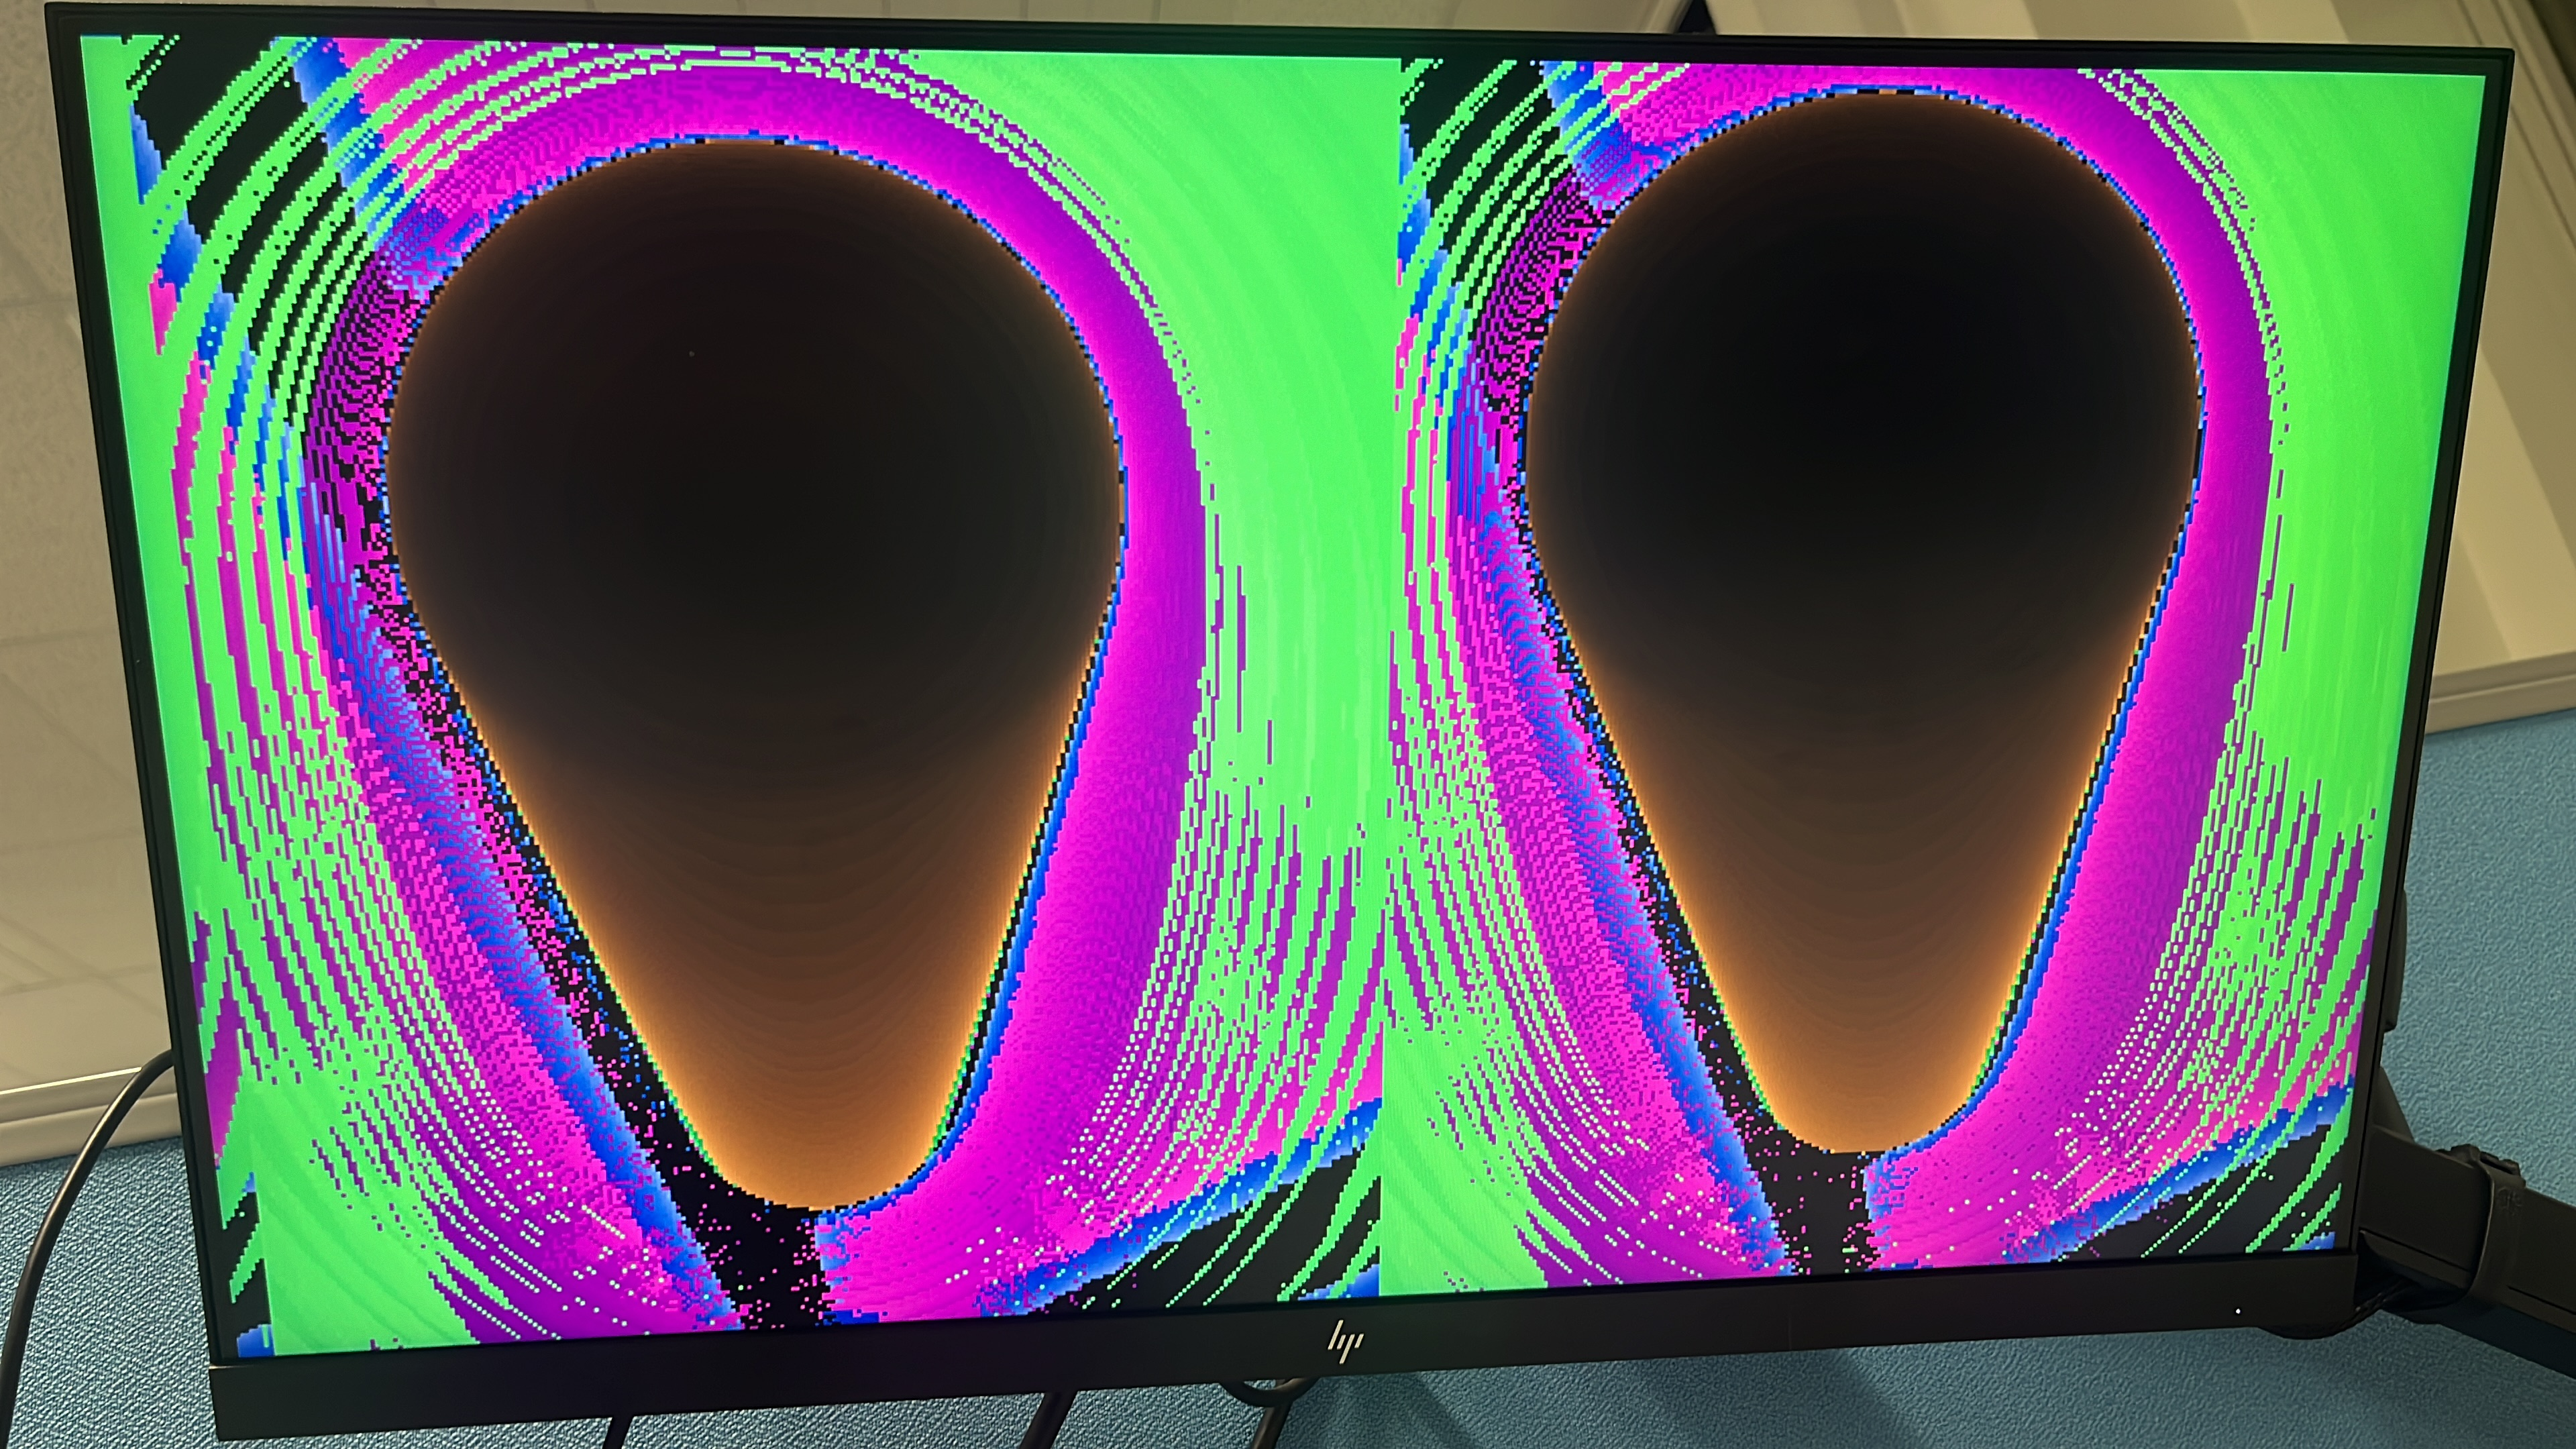
\includegraphics[width=\textwidth,height=0.28\textheight,keepaspectratio]{imgs/AppendixA/render_hyperboloid_stereo.jpg}
    \caption{Capsule SDF, single-sheet geometry. Large teardrop profile against green--purple background.}
\end{subfigure}

\vfill

\begin{subfigure}[b]{0.48\textwidth}
    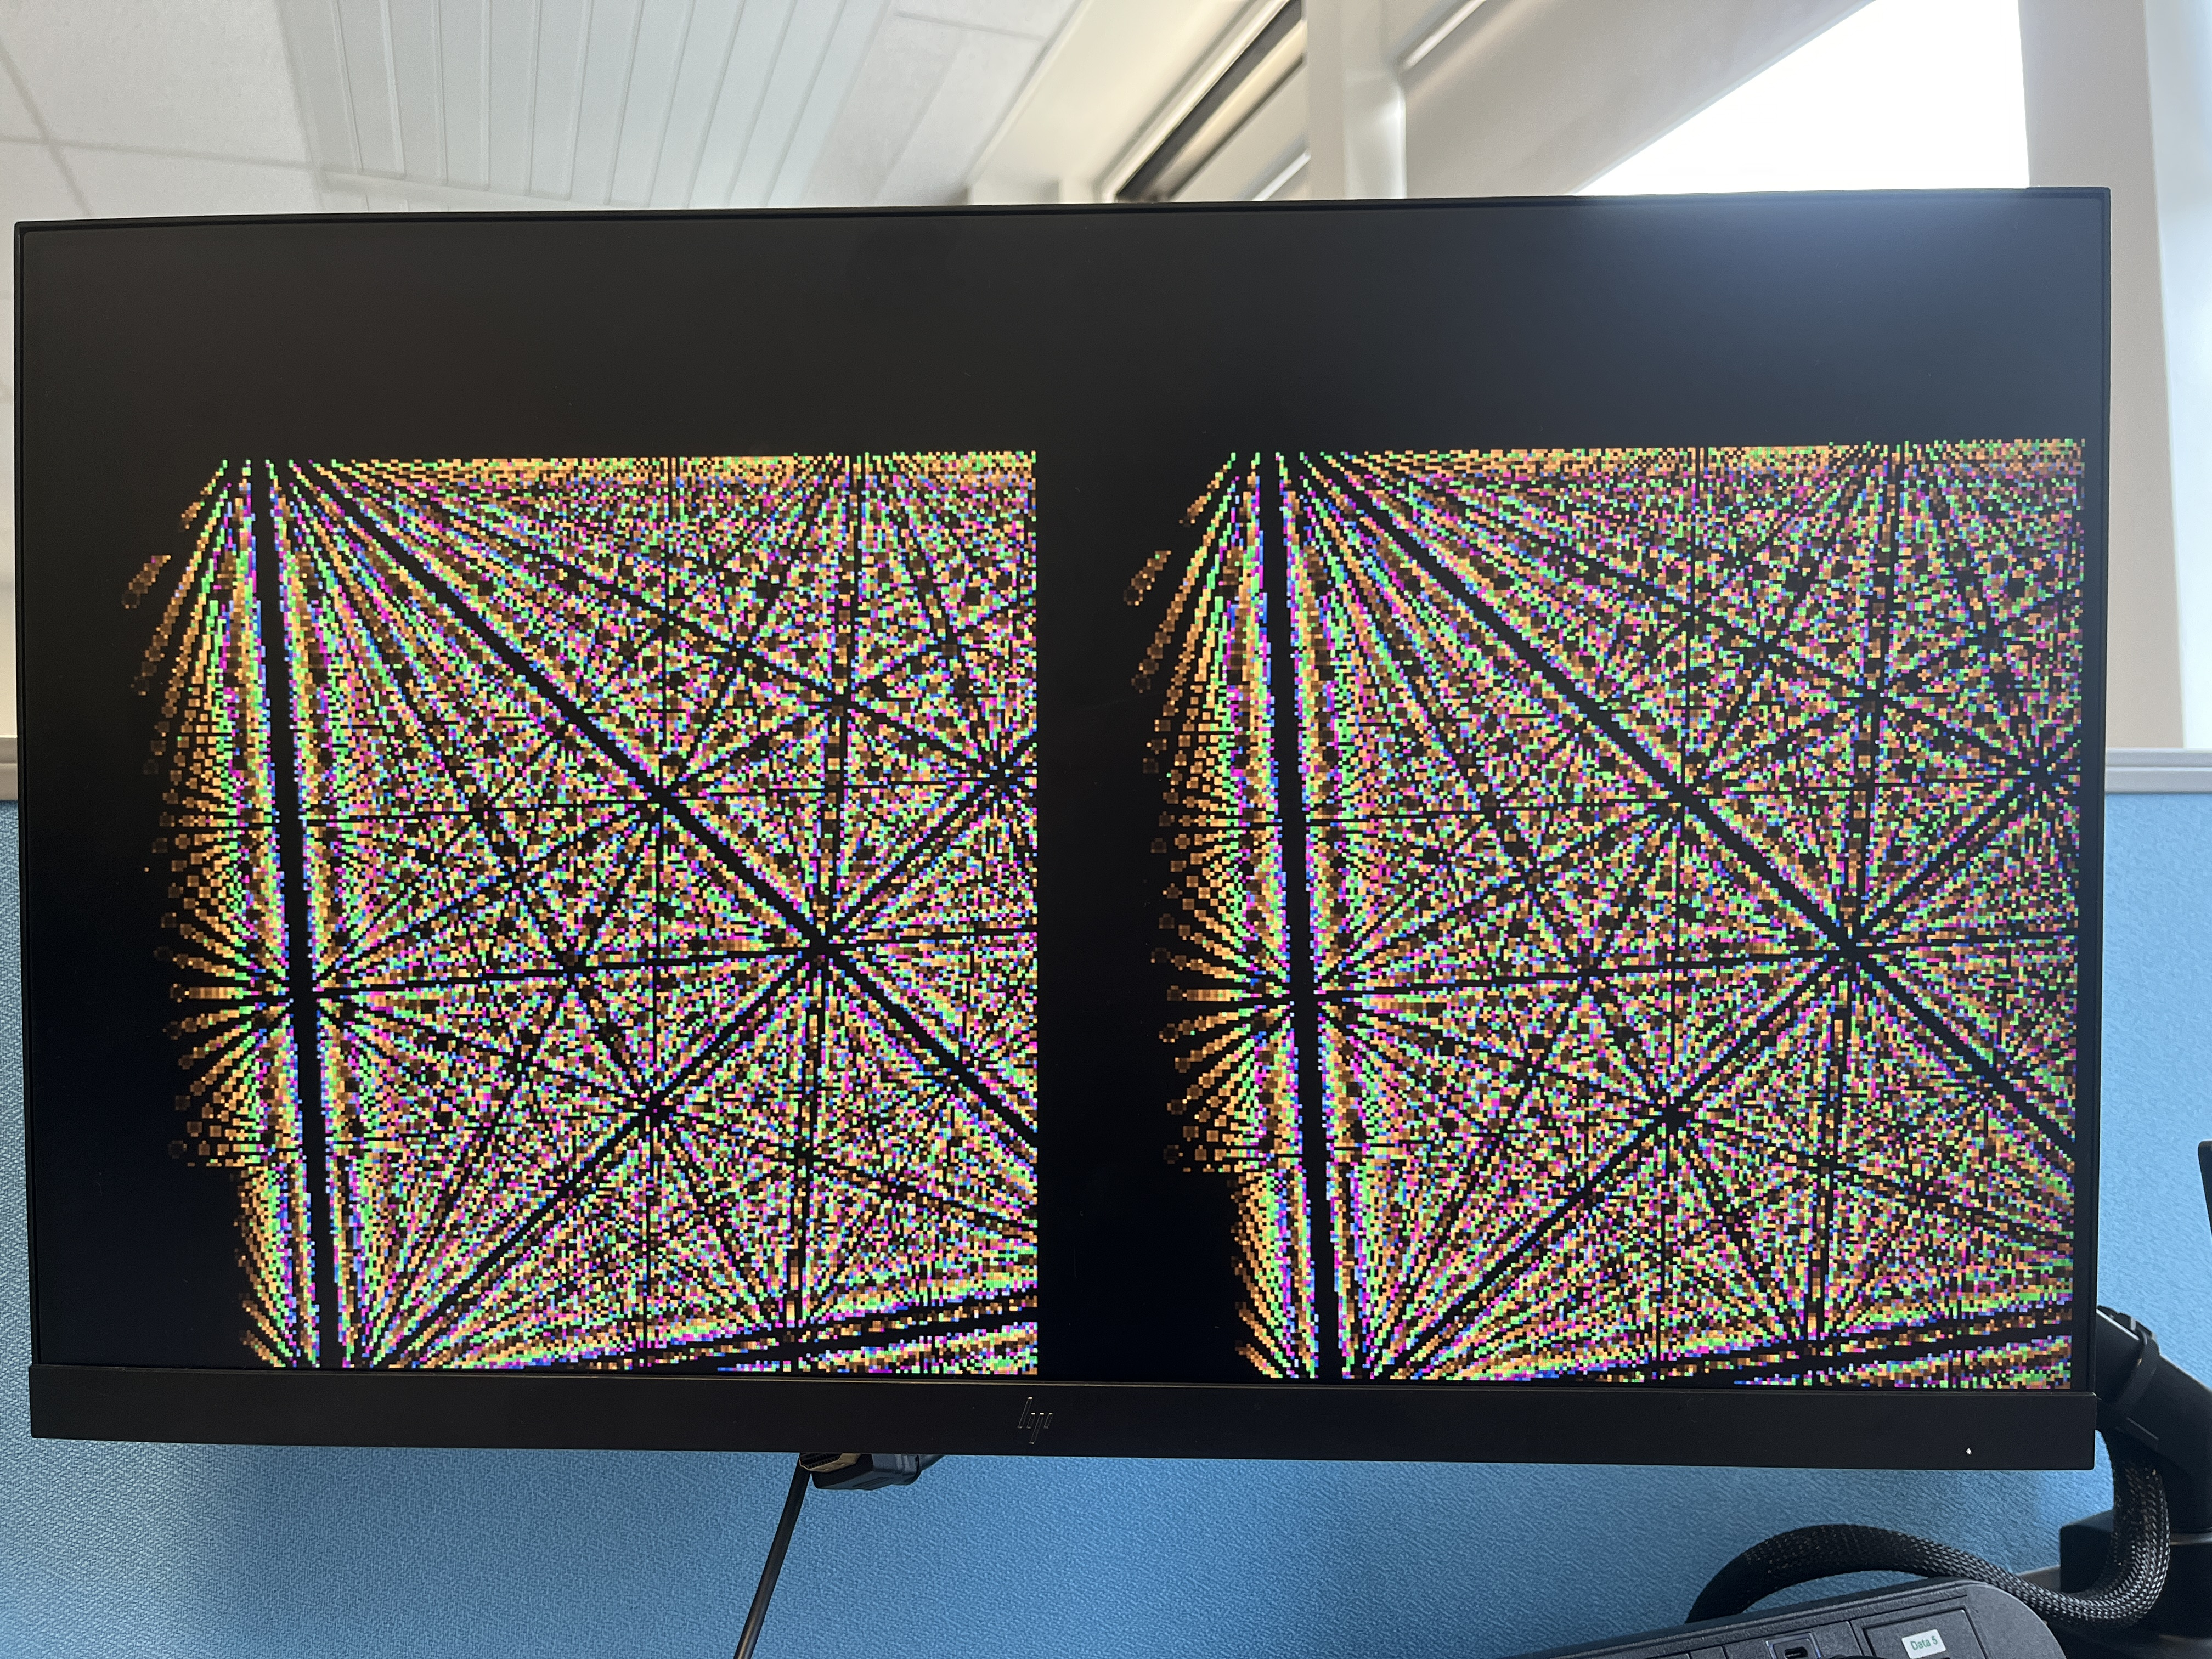
\includegraphics[width=\textwidth,height=0.28\textheight,keepaspectratio]{imgs/AppendixA/render_scaffold_lattice_stereo.jpg}
    \caption{Sphere box-frame lattice on black background. Diamond grid from space repetition, \texttt{cell\_size} $= 2$.}
\end{subfigure}\hfill
\begin{subfigure}[b]{0.48\textwidth}
    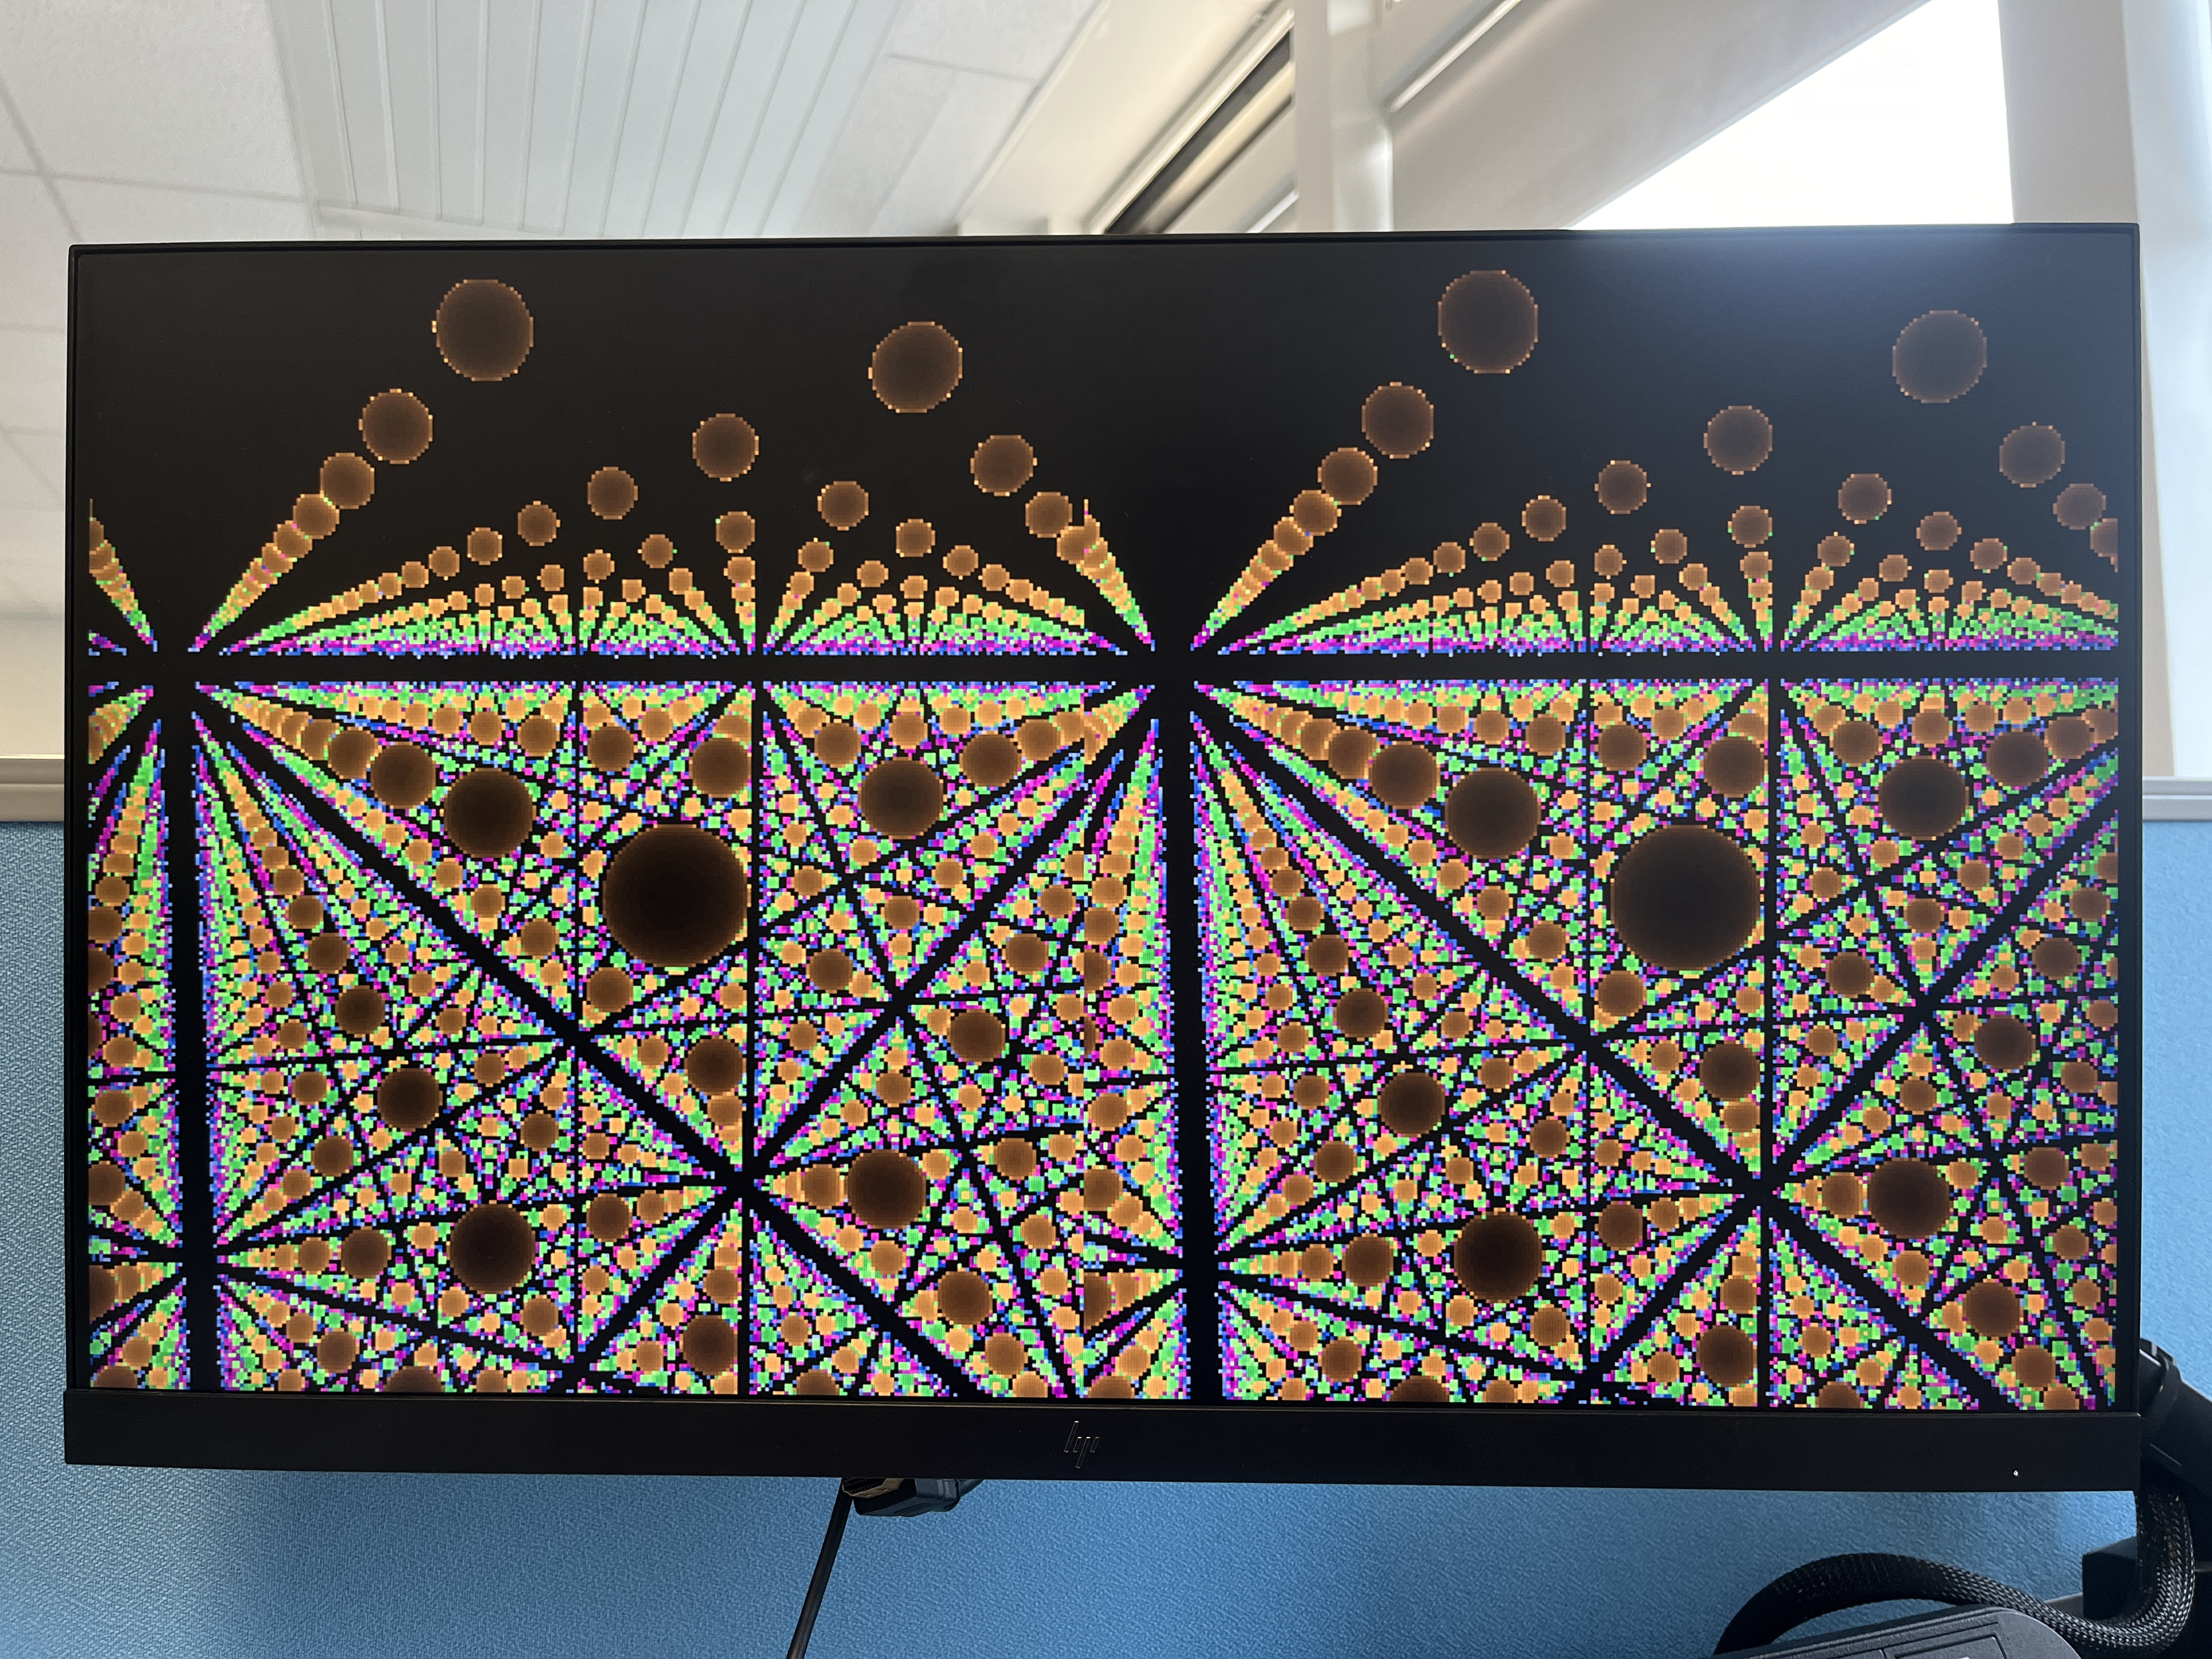
\includegraphics[width=\textwidth,height=0.28\textheight,keepaspectratio]{imgs/AppendixA/render_gyroid_spheres_stereo.jpg}
    \caption{Sphere with space-repeated sphere array. Infinite lattice viewed from close range, \texttt{cell\_size} $= 10$.}
\end{subfigure}
\caption{Stereoscopic render gallery I: early hardware output on external monitor.}
\end{figure}

\clearpage

% ----------------------------------------------------------------
%  Page 2 — Mandelbox variants + gyroid spheres variant + headset
% ----------------------------------------------------------------
\begin{figure}[H]
\vspace*{-0.5cm}
\centering
\begin{subfigure}[b]{0.48\textwidth}
    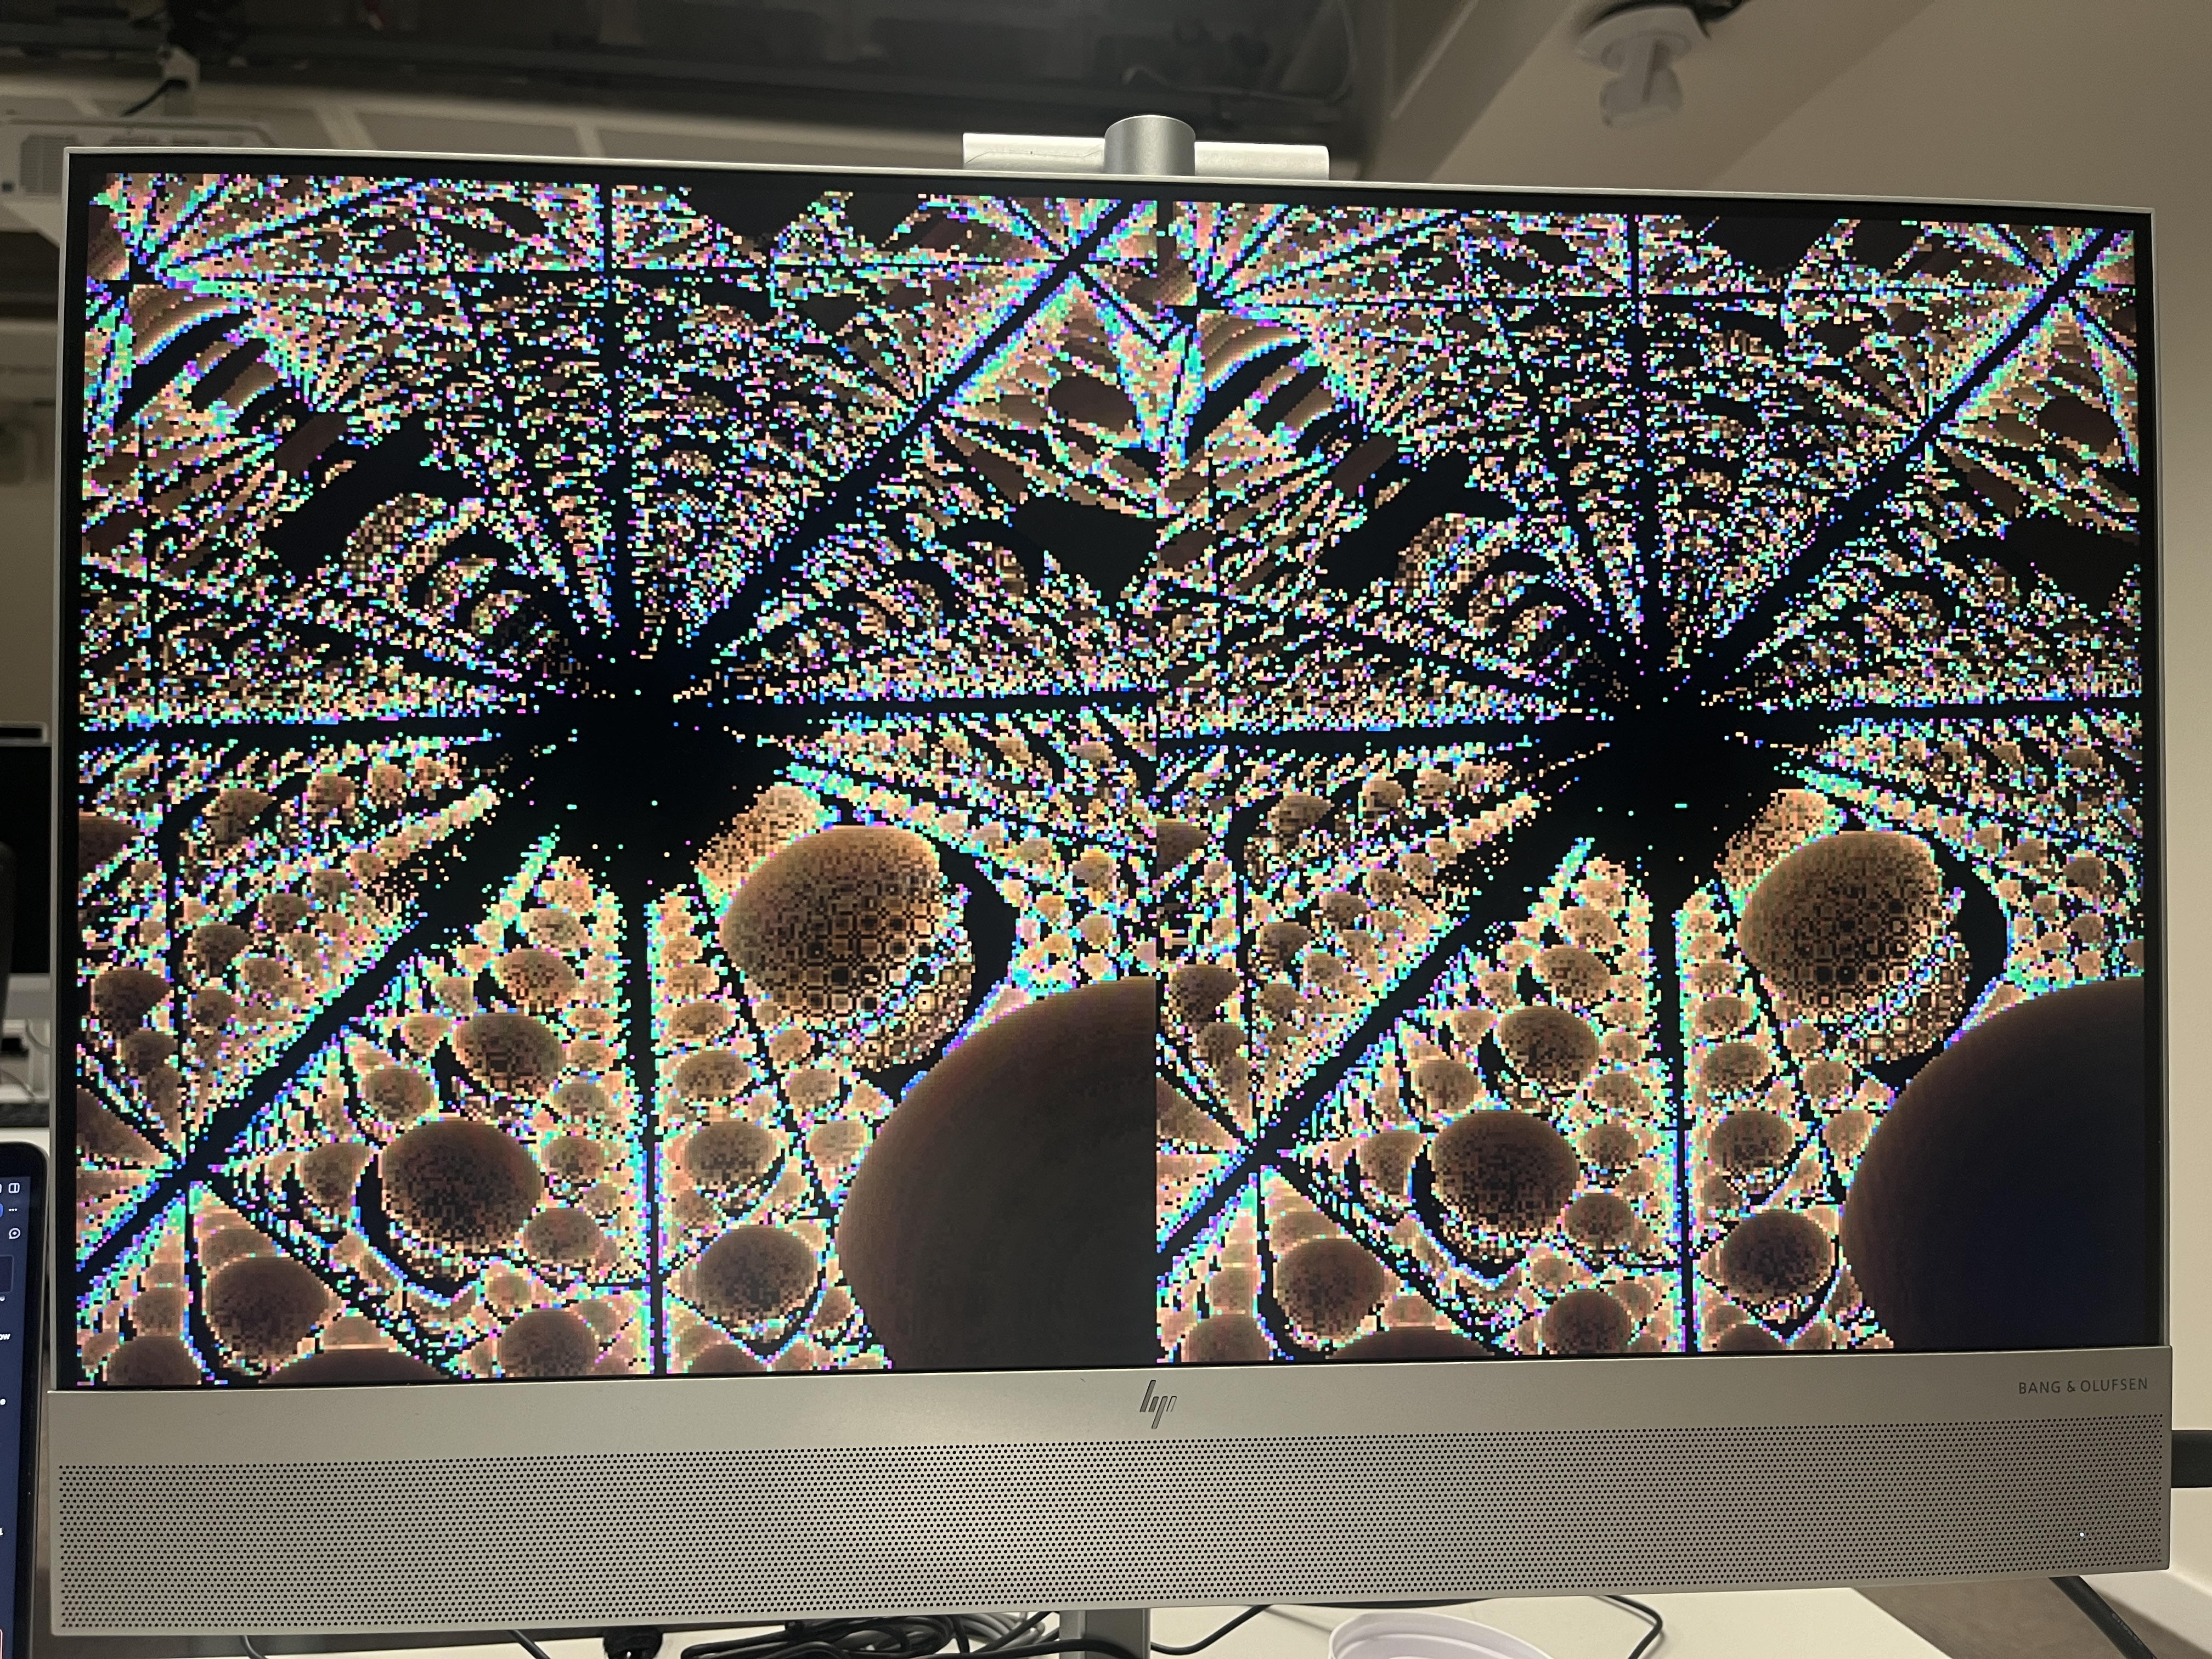
\includegraphics[width=\textwidth,height=0.28\textheight,keepaspectratio]{imgs/AppendixA/render_mandelbox_closeup_stereo.jpg}
    \caption{Sphere boundary close-up. Spiky self-similar structures at the exterior box-fold boundary due to approximations in NR}
\end{subfigure}\hfill
\begin{subfigure}[b]{0.48\textwidth}
    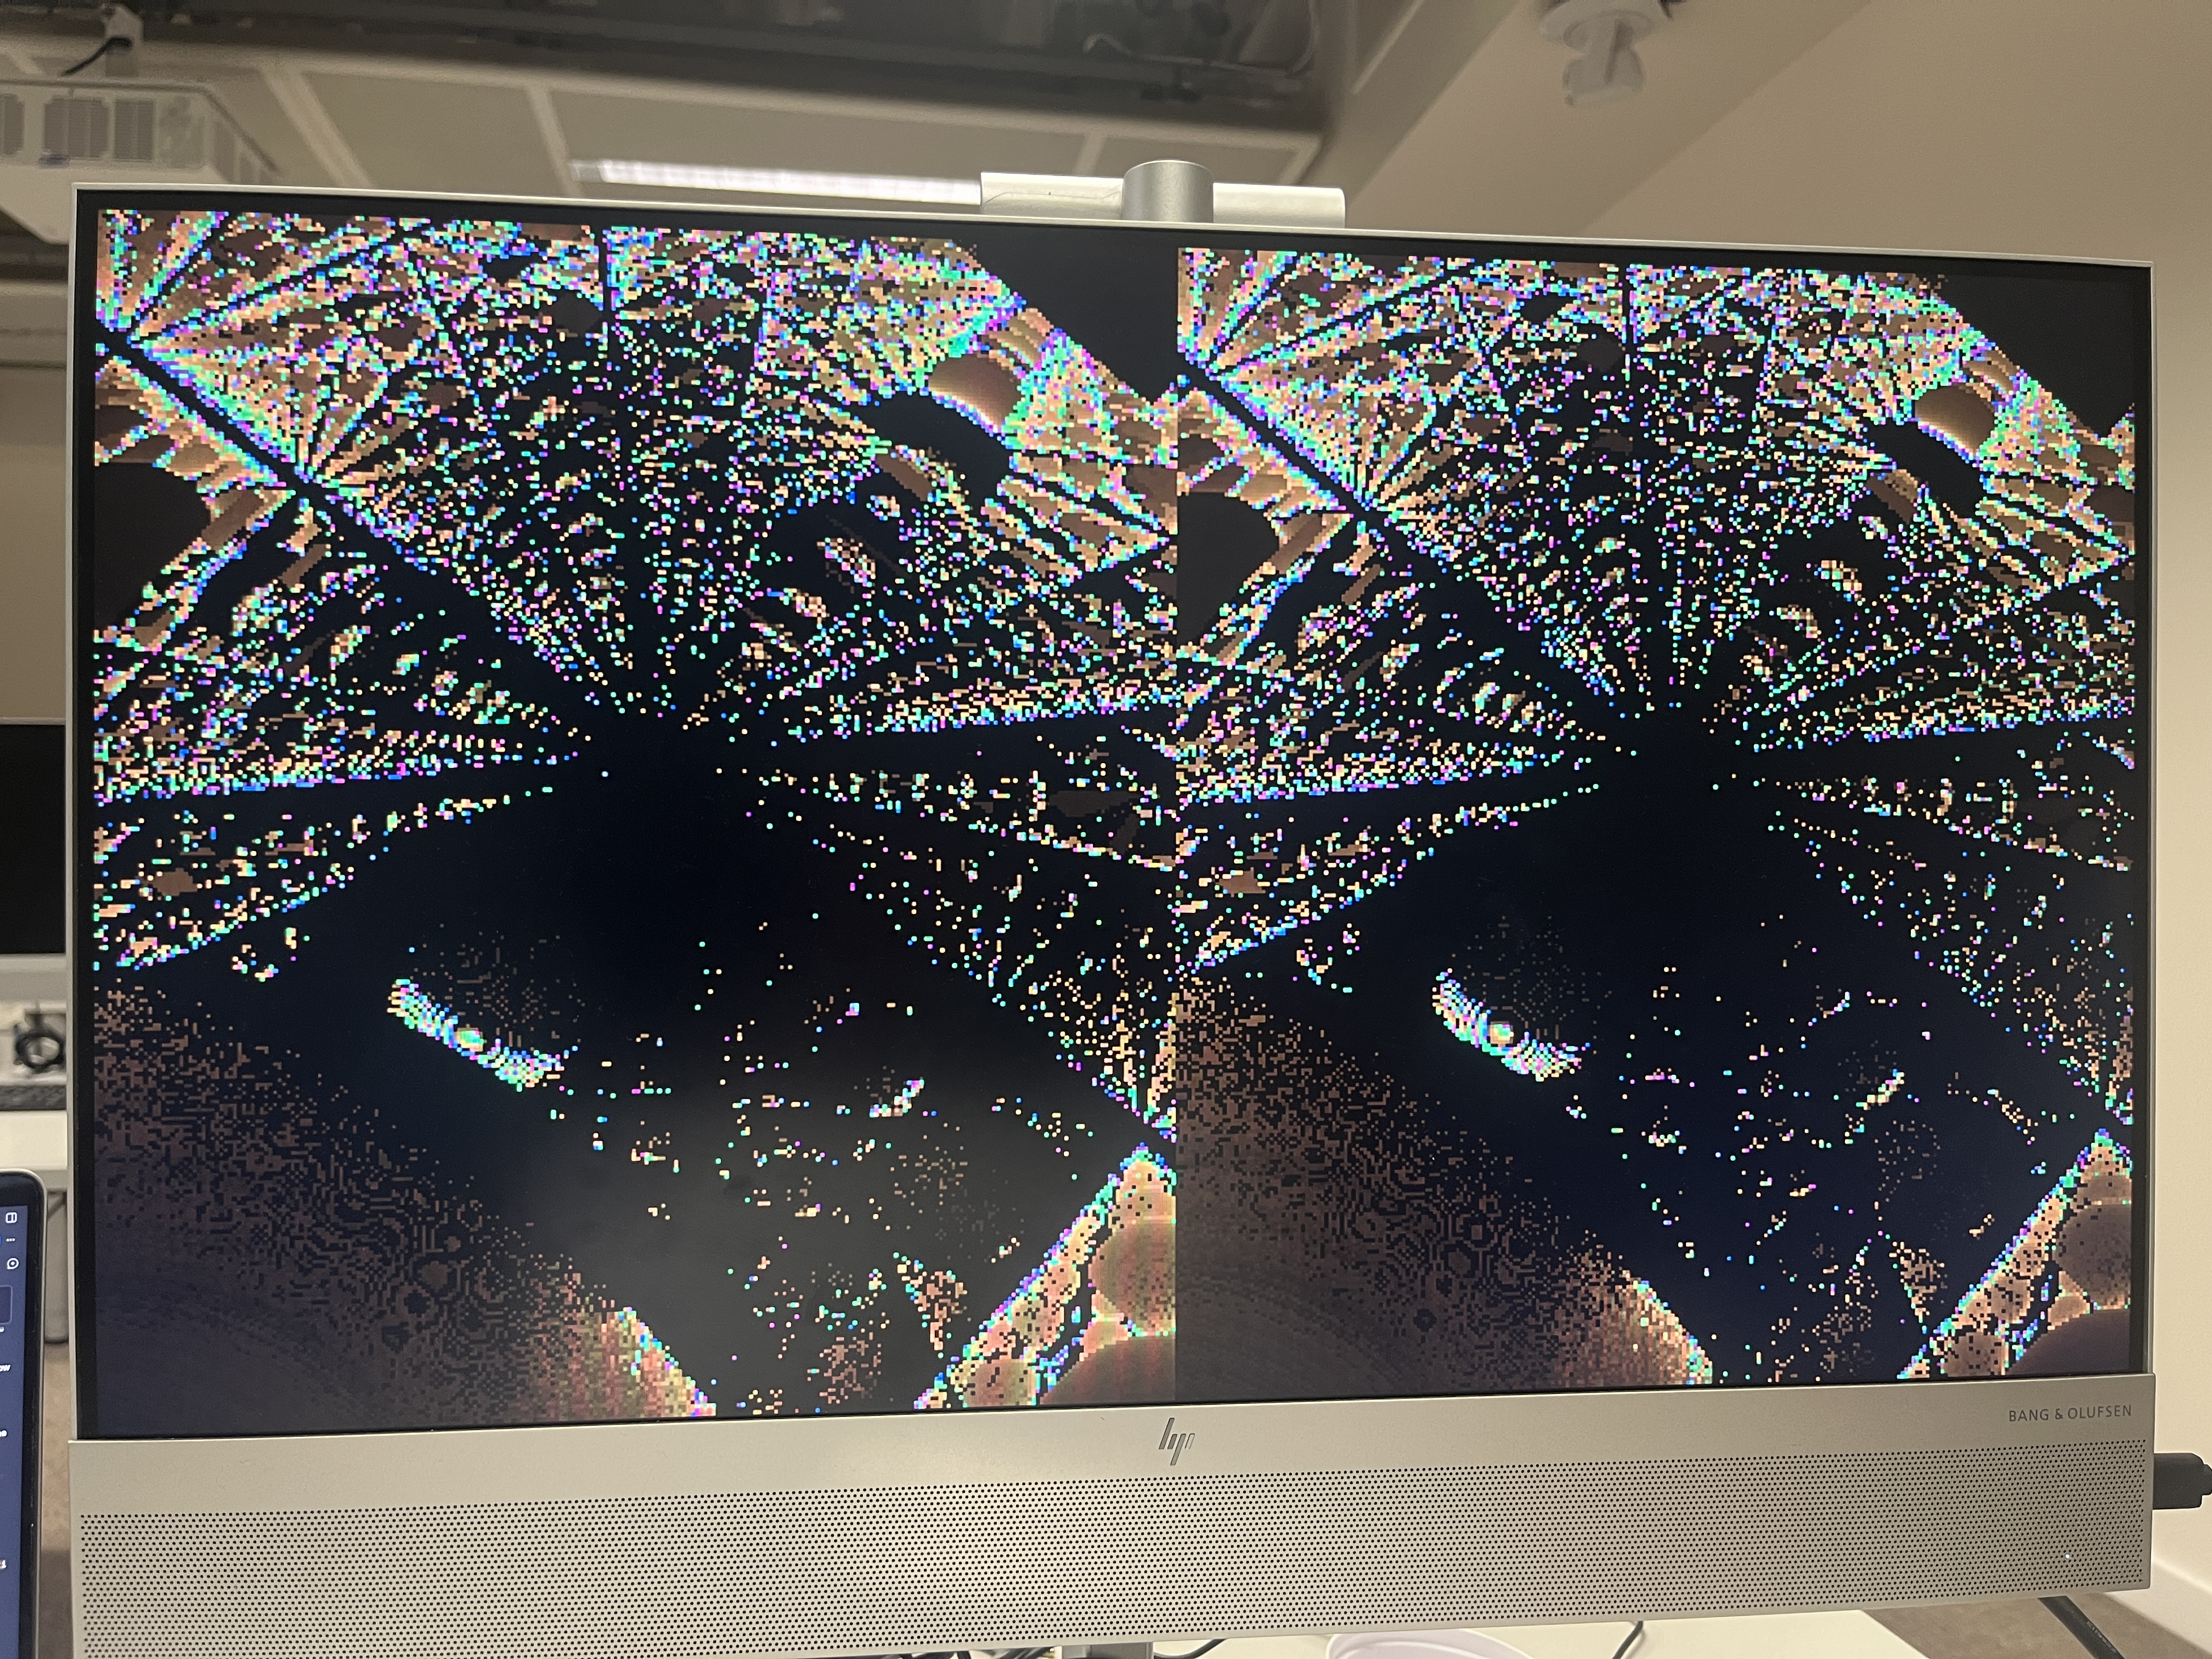
\includegraphics[width=\textwidth,height=0.28\textheight,keepaspectratio]{imgs/AppendixA/render_mandelbox_interior_stereo.jpg}
    \caption{NR approximations acculumations.}
\end{subfigure}

\vfill

\begin{subfigure}[b]{0.48\textwidth}
    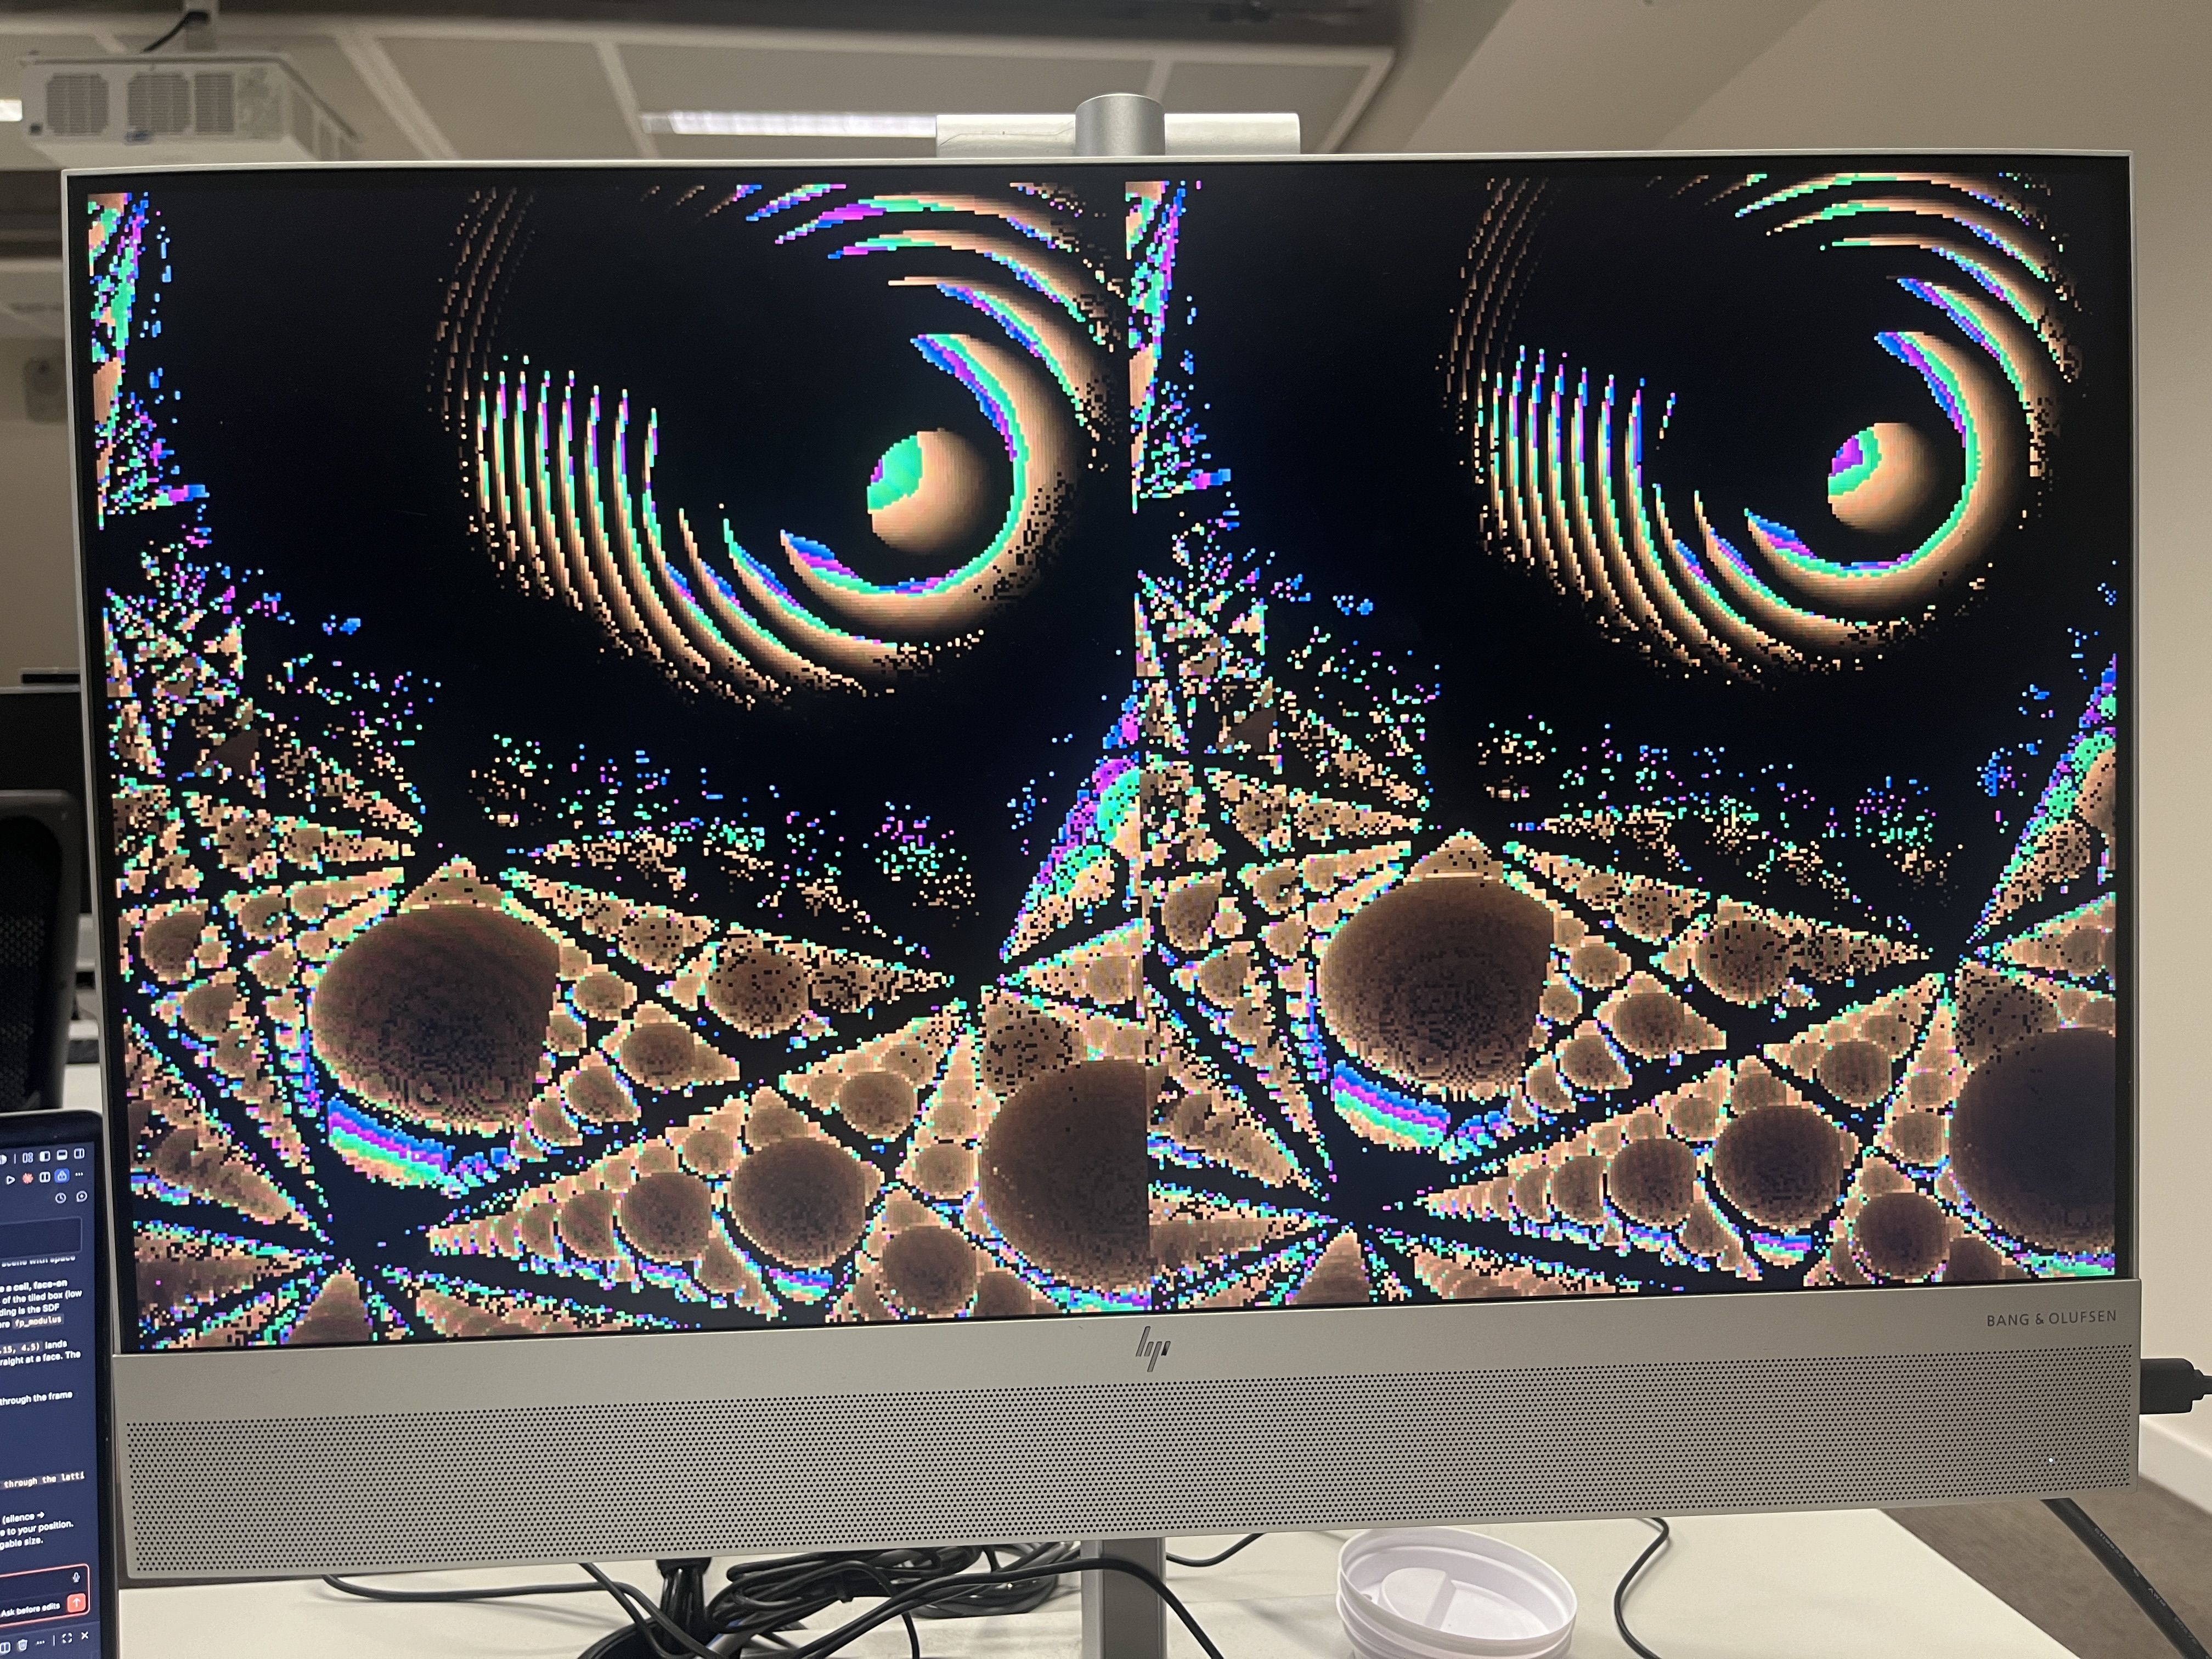
\includegraphics[width=\textwidth,height=0.28\textheight,keepaspectratio]{imgs/AppendixA/render_mandelbox_spiral_stereo.jpg}
    \caption{NR approximations acculumations.}
\end{subfigure}\hfill
\begin{subfigure}[b]{0.48\textwidth}
    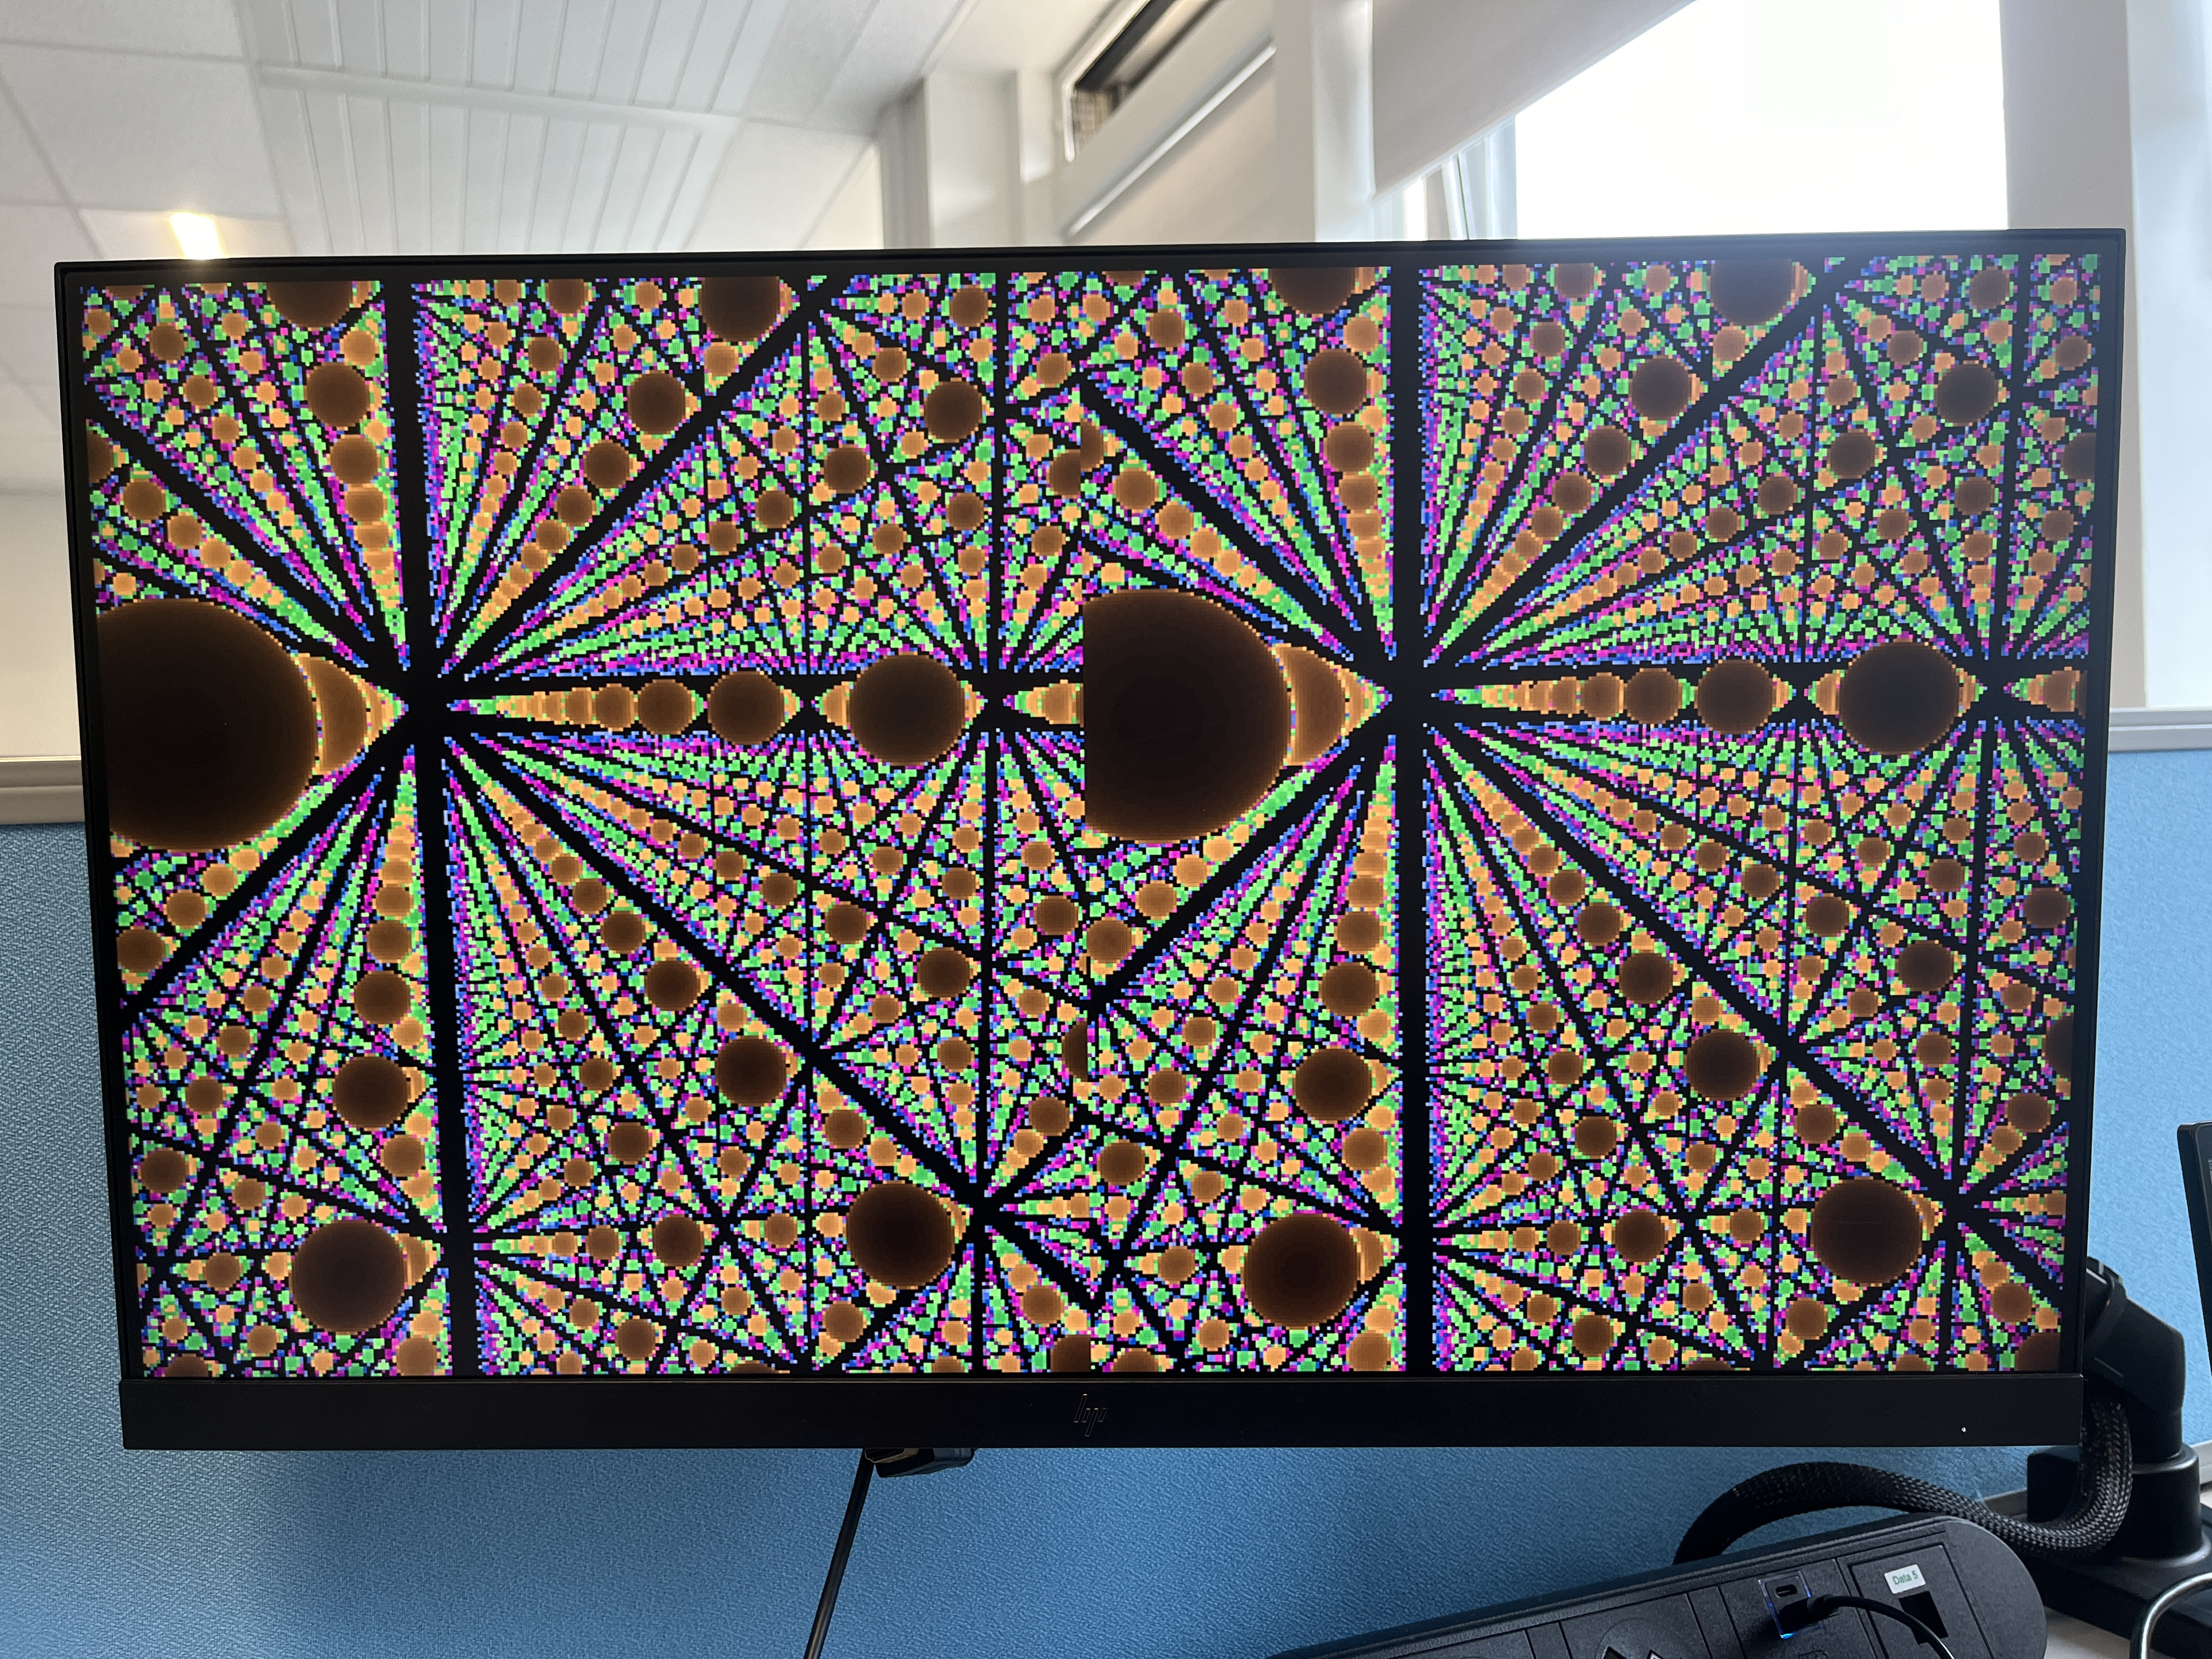
\includegraphics[width=\textwidth,height=0.28\textheight,keepaspectratio]{imgs/AppendixA/render_mandelbox_lattice_stereo.jpg}
    \caption{Infinite spheres, space-repeated with \texttt{cell\_size} $= 2$.}
\end{subfigure}

\vfill

\begin{subfigure}[b]{0.48\textwidth}
    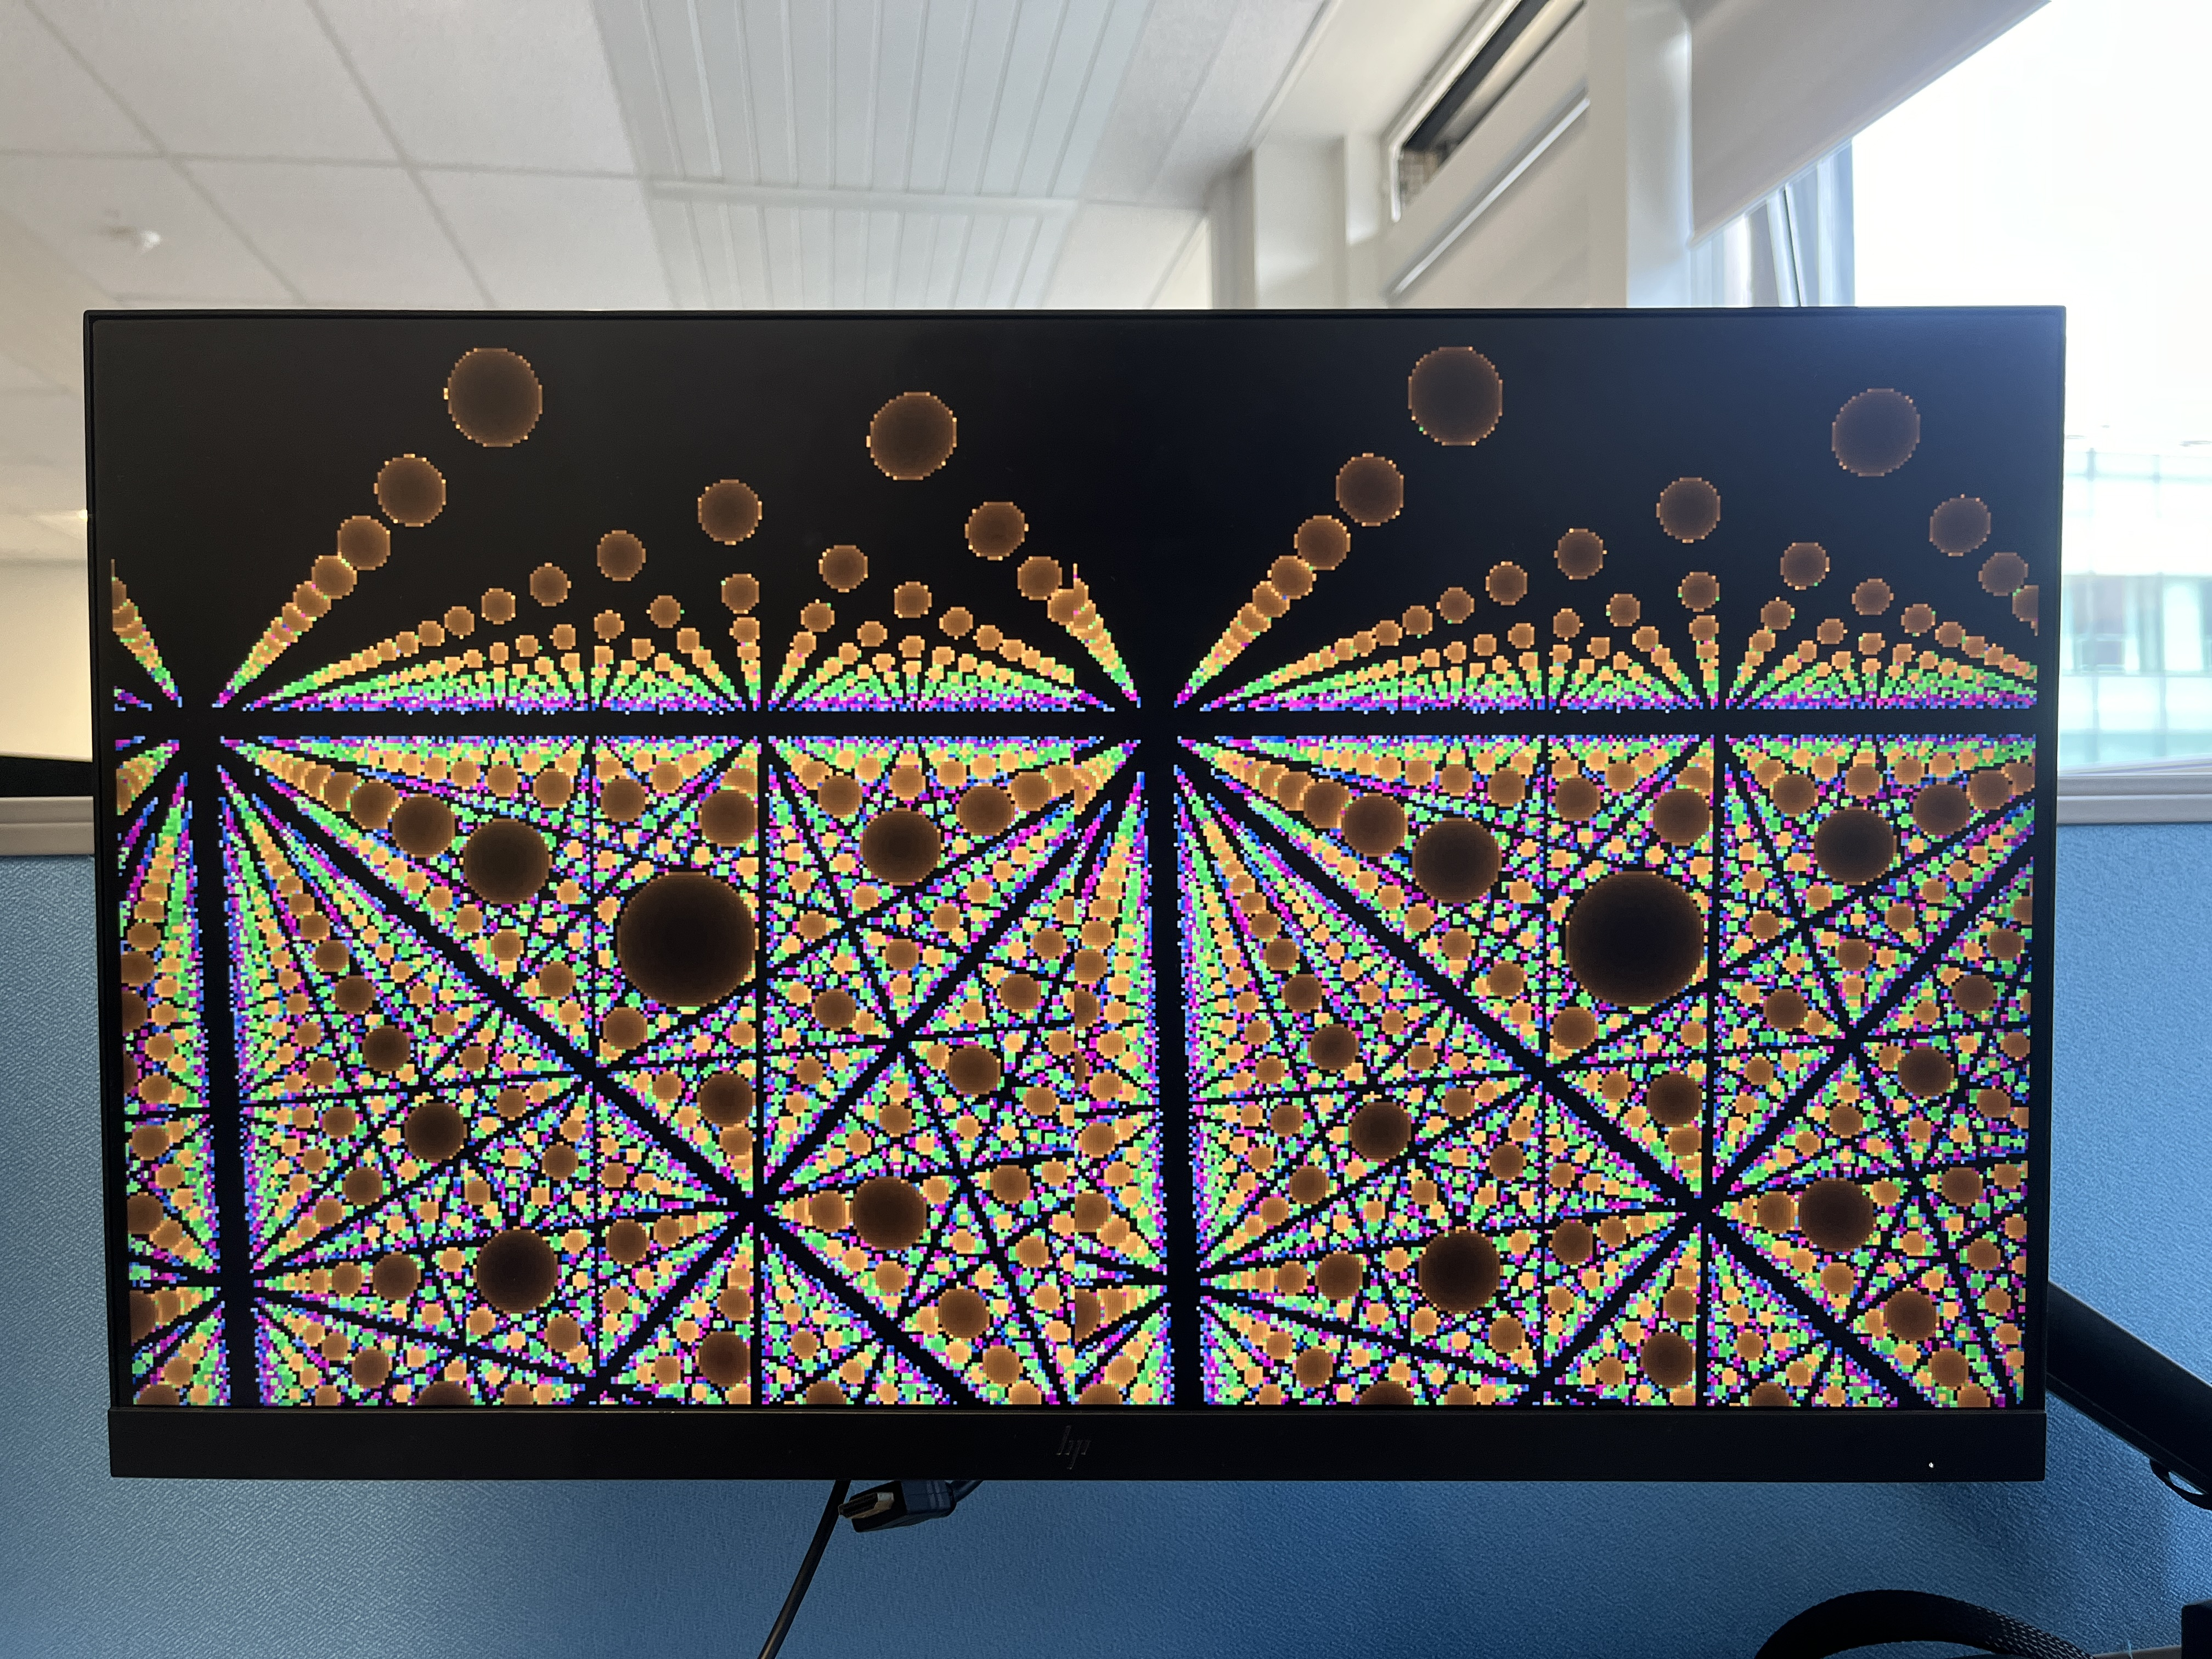
\includegraphics[width=\textwidth,height=0.28\textheight,keepaspectratio]{imgs/AppendixA/render_gyroid_spheres2_stereo.jpg}
    \caption{Infinite Spheres}
\end{subfigure}\hfill
\begin{subfigure}[b]{0.48\textwidth}
    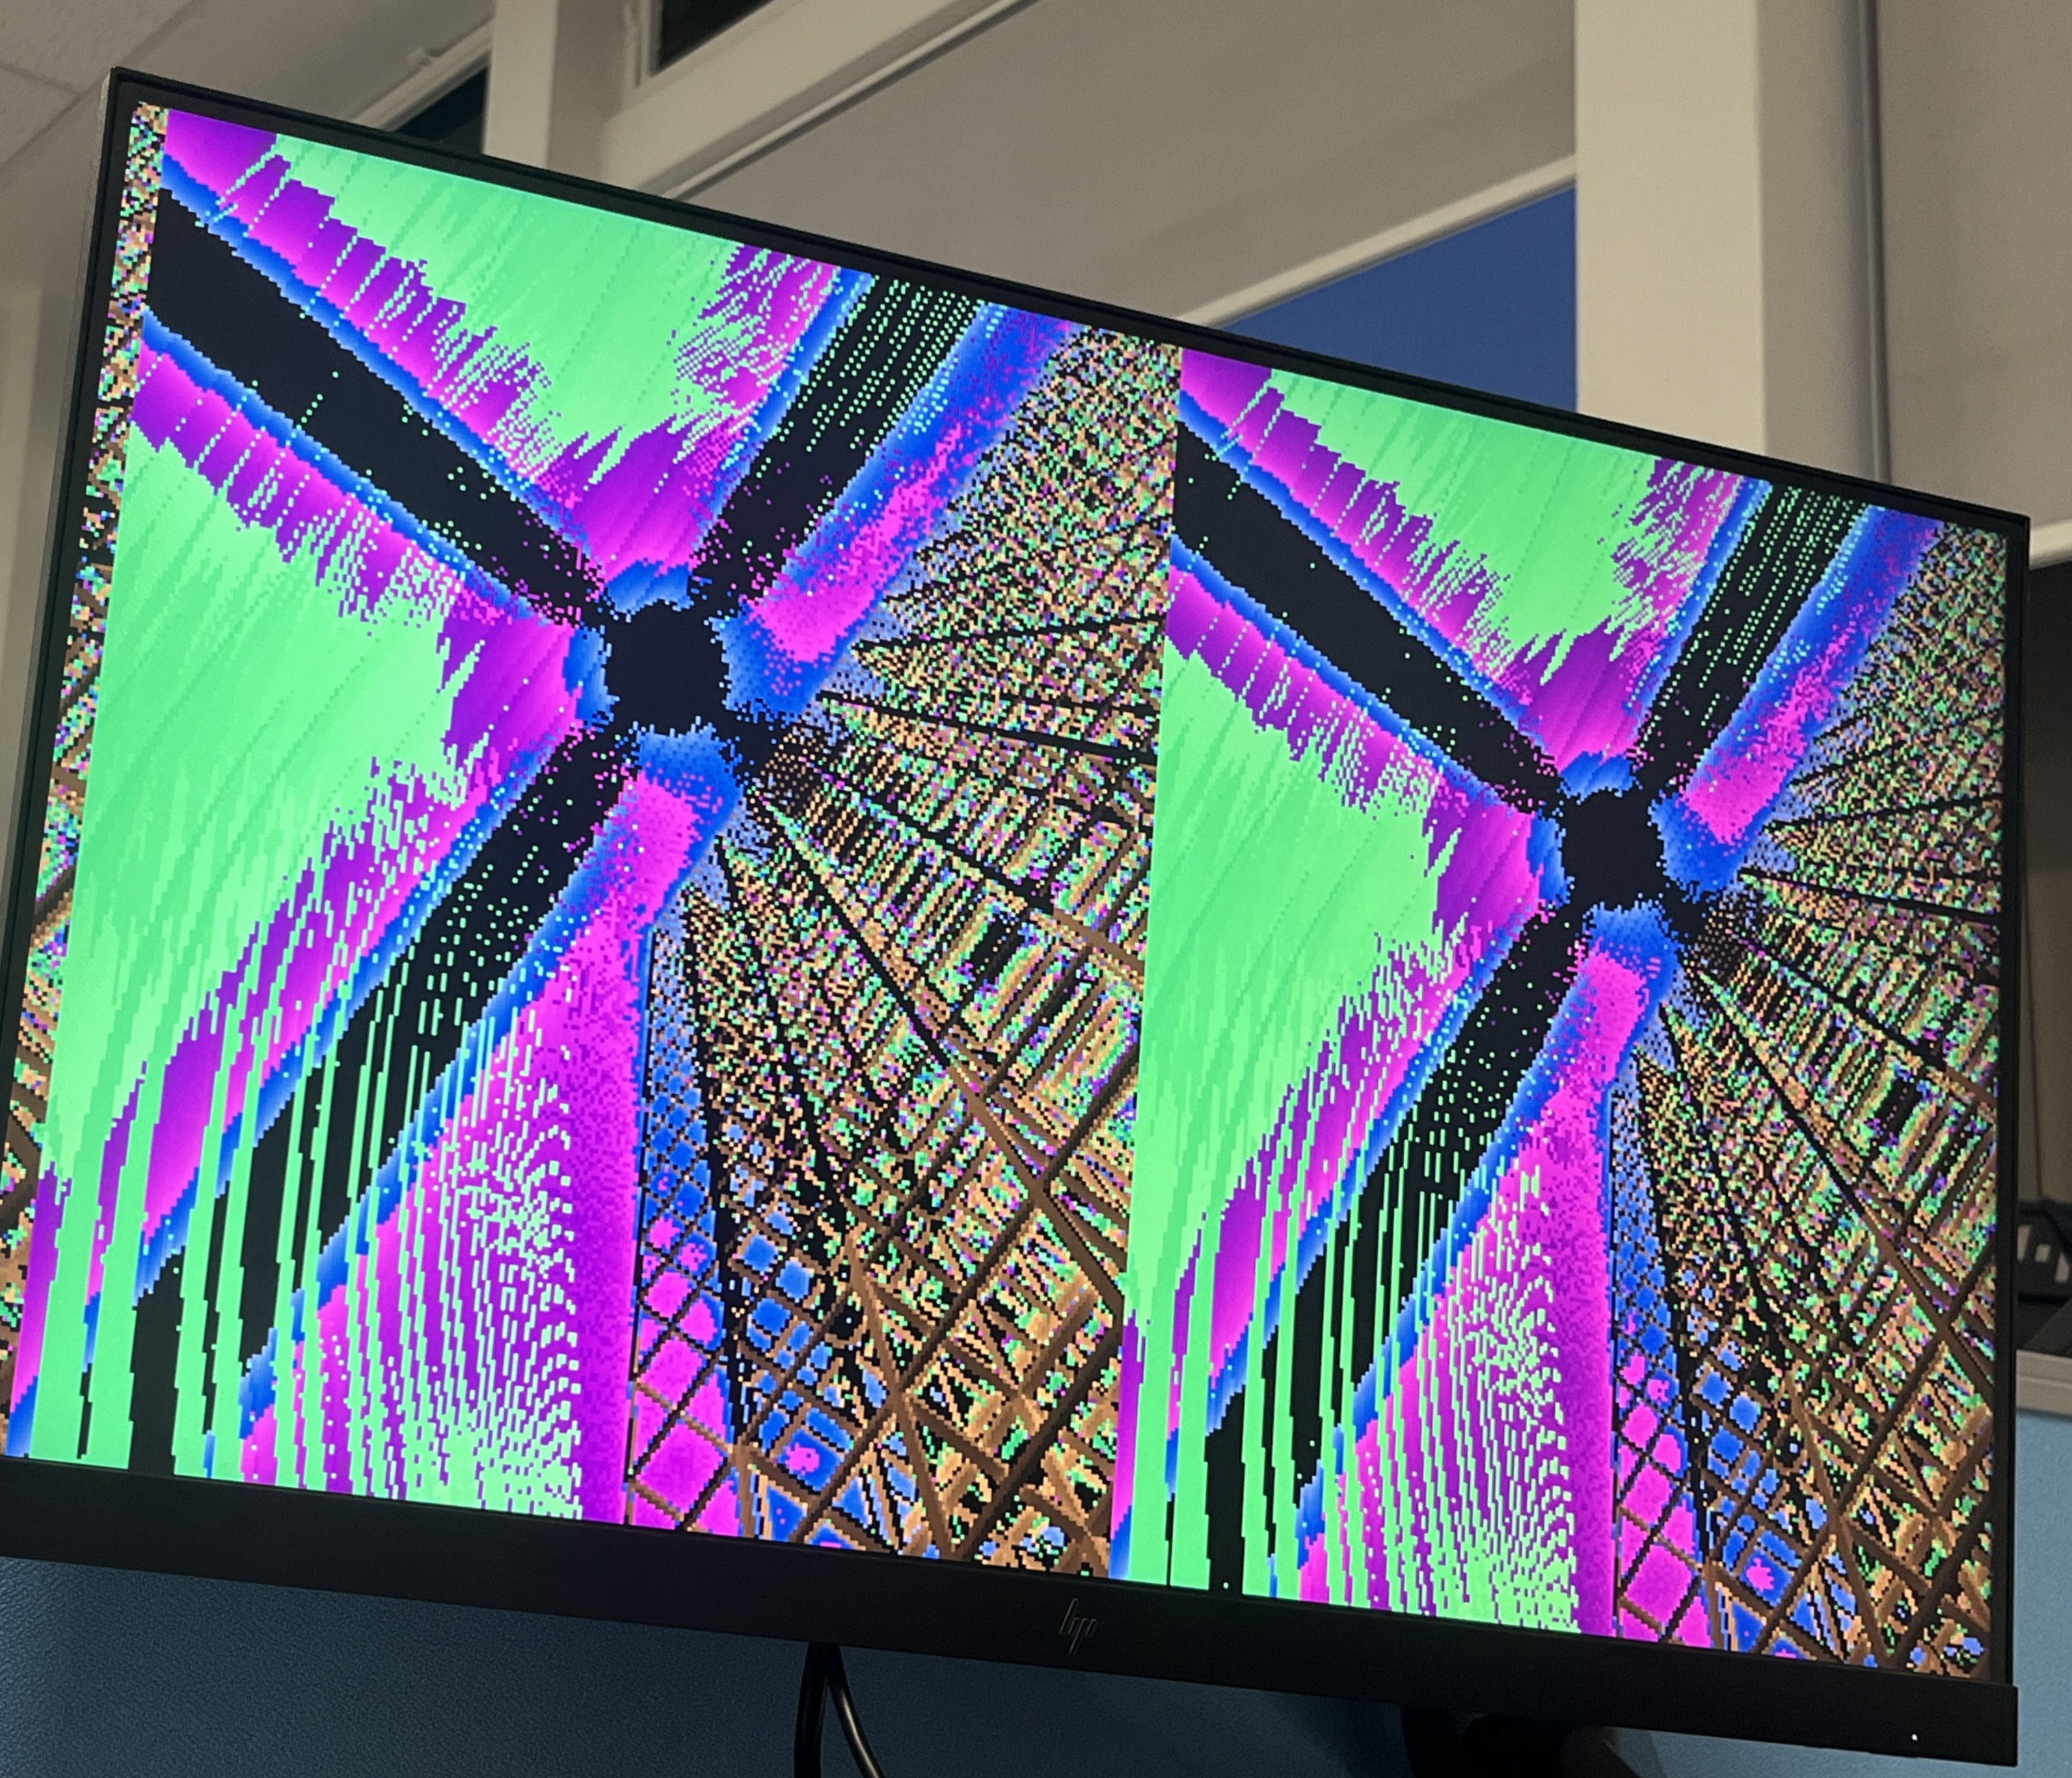
\includegraphics[width=\textwidth,height=0.28\textheight,keepaspectratio]{imgs/AppendixA/headset_photo_1.jpg}
    \caption{Assembled VR headset prototype, front view. FPGA friction-fitted into custom 3D-printed chassis.}
\end{subfigure}
\caption{Stereoscopic render gallery II: Mandelbox variants and assembled headset.}
\end{figure}

\clearpage

% ----------------------------------------------------------------
%  Page 3 — New scaffold stereo board photos (5) + headset photo 2
% ----------------------------------------------------------------
\begin{figure}[H]
\vspace*{-0.5cm}
\centering
\begin{subfigure}[b]{0.48\textwidth}
    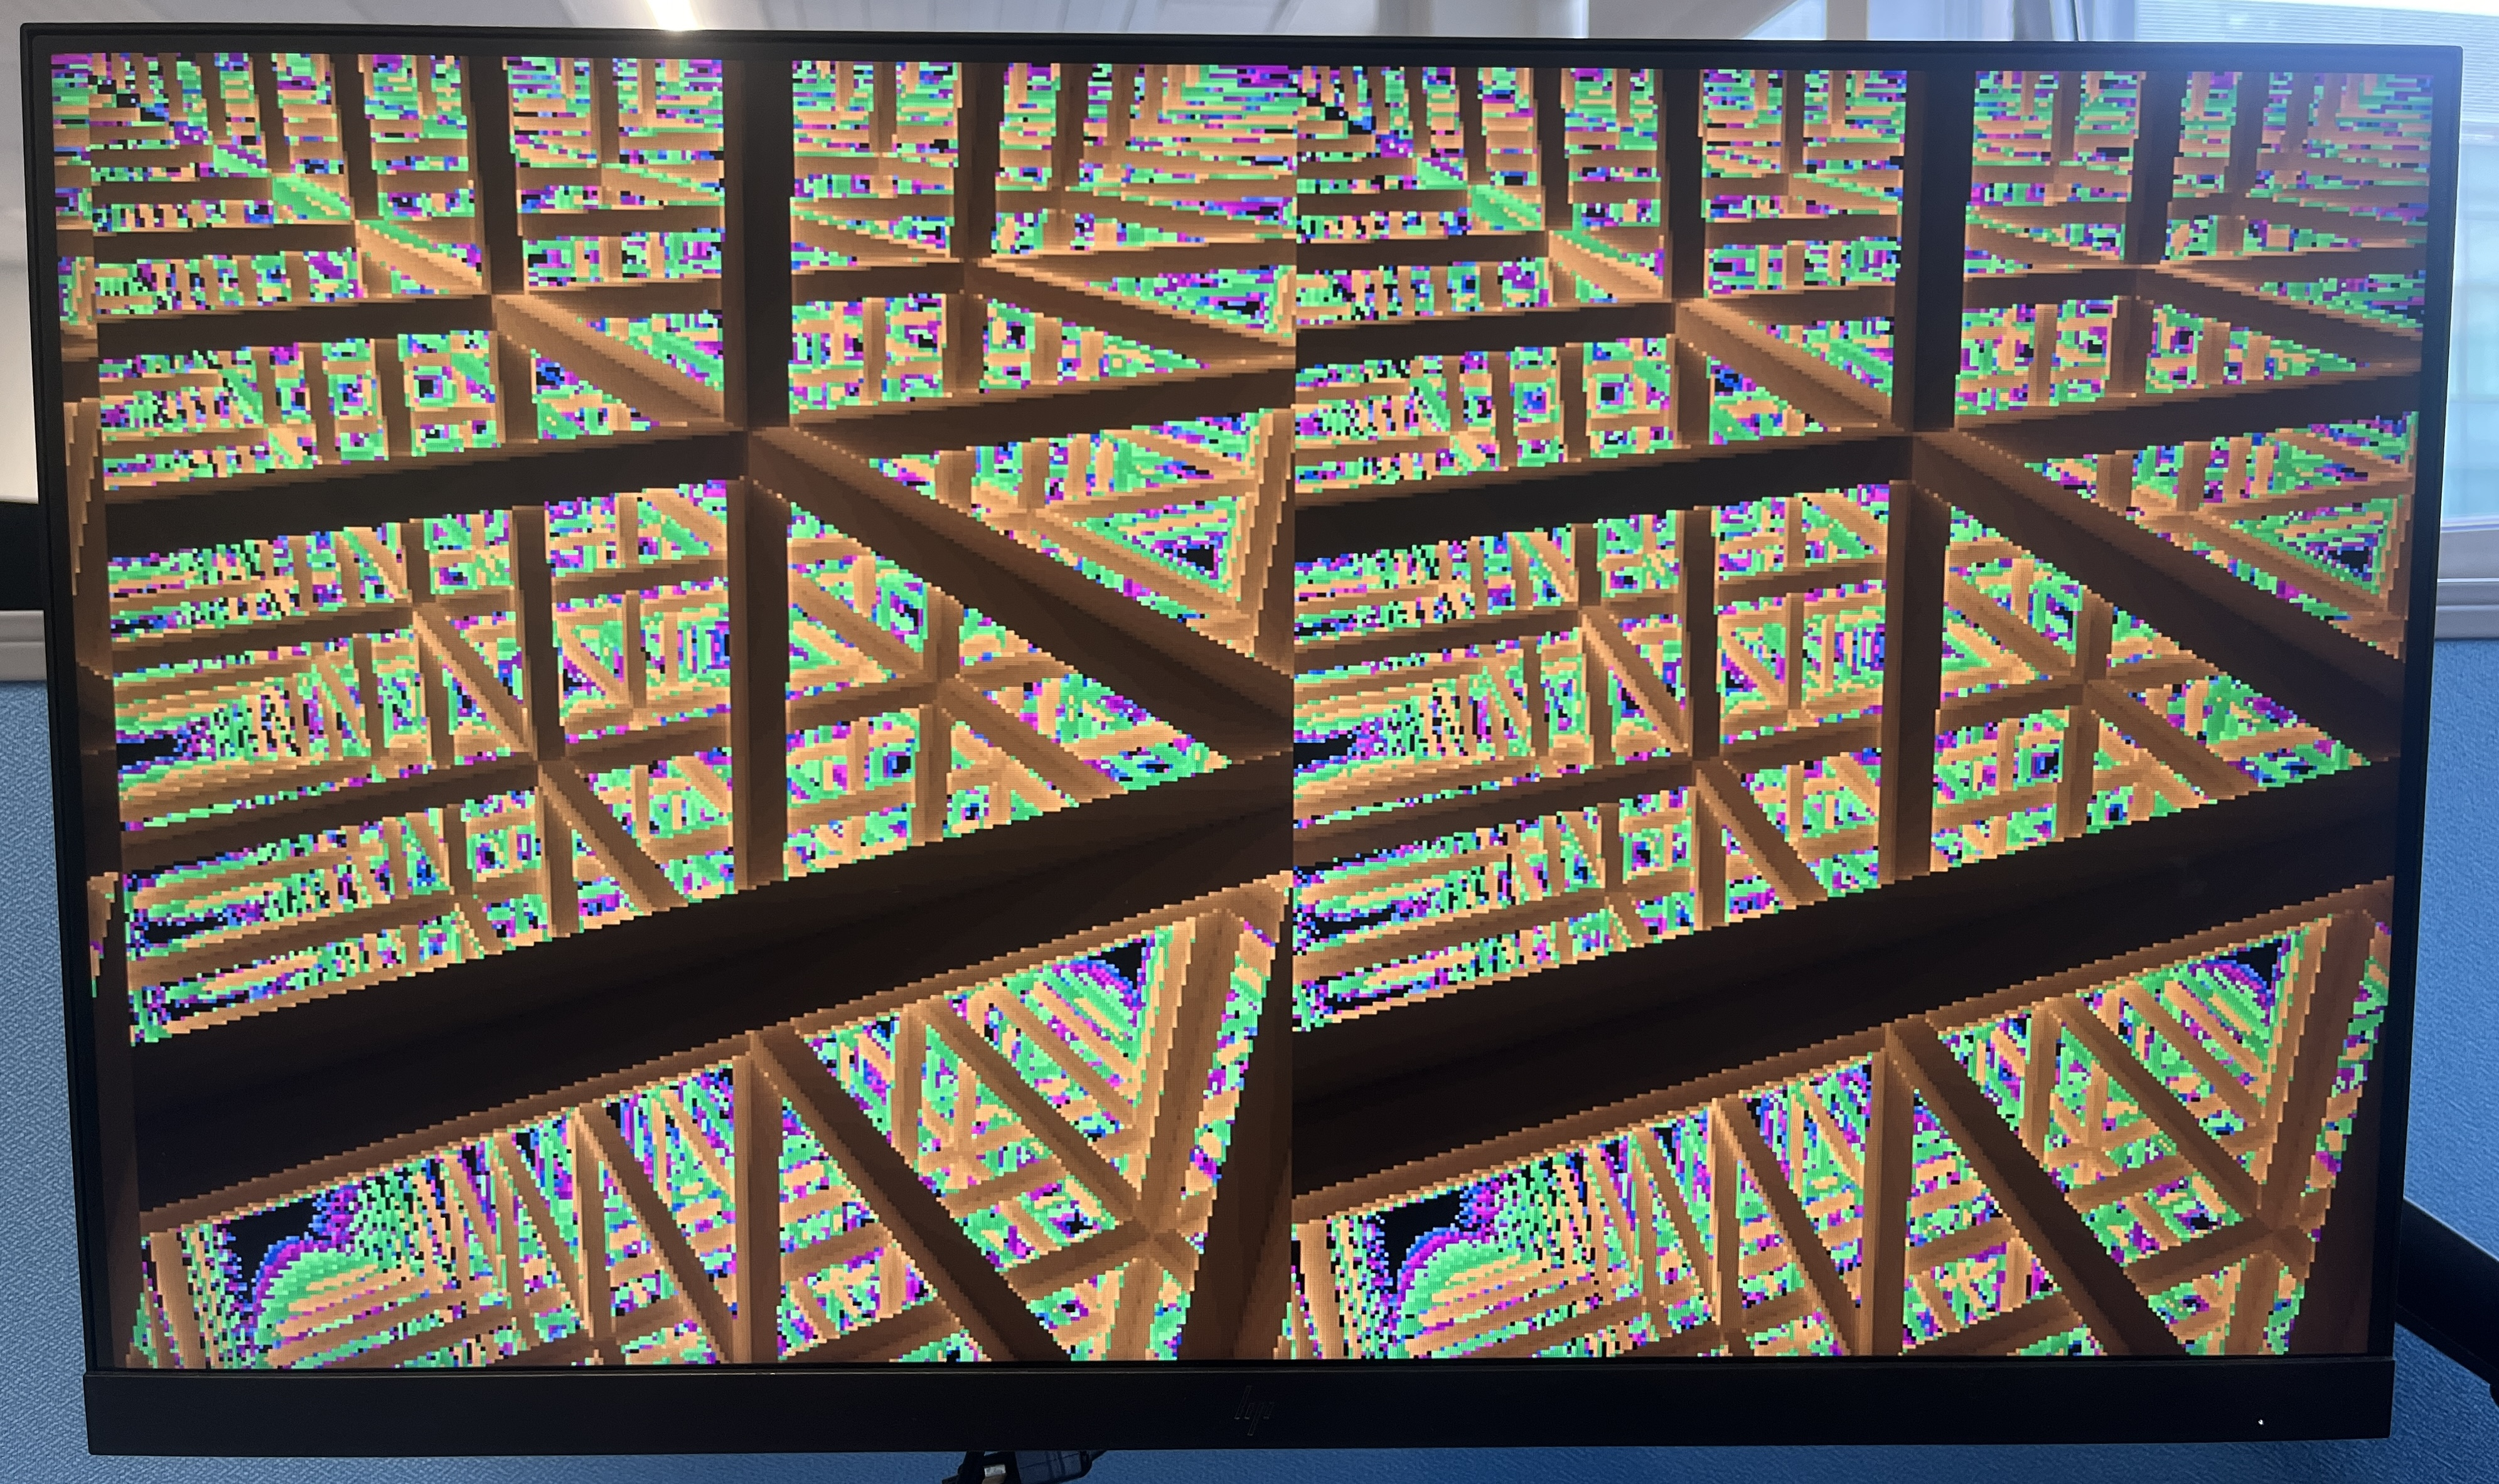
\includegraphics[width=\textwidth,height=0.28\textheight,keepaspectratio]{imgs/AppendixA/render_scaffold_overhead_stereo.jpg}
    \caption{Scaffold box-frame from an oblique overhead angle. Infinite lattice depth visible across the stereo pair.}
\end{subfigure}\hfill
\begin{subfigure}[b]{0.48\textwidth}
    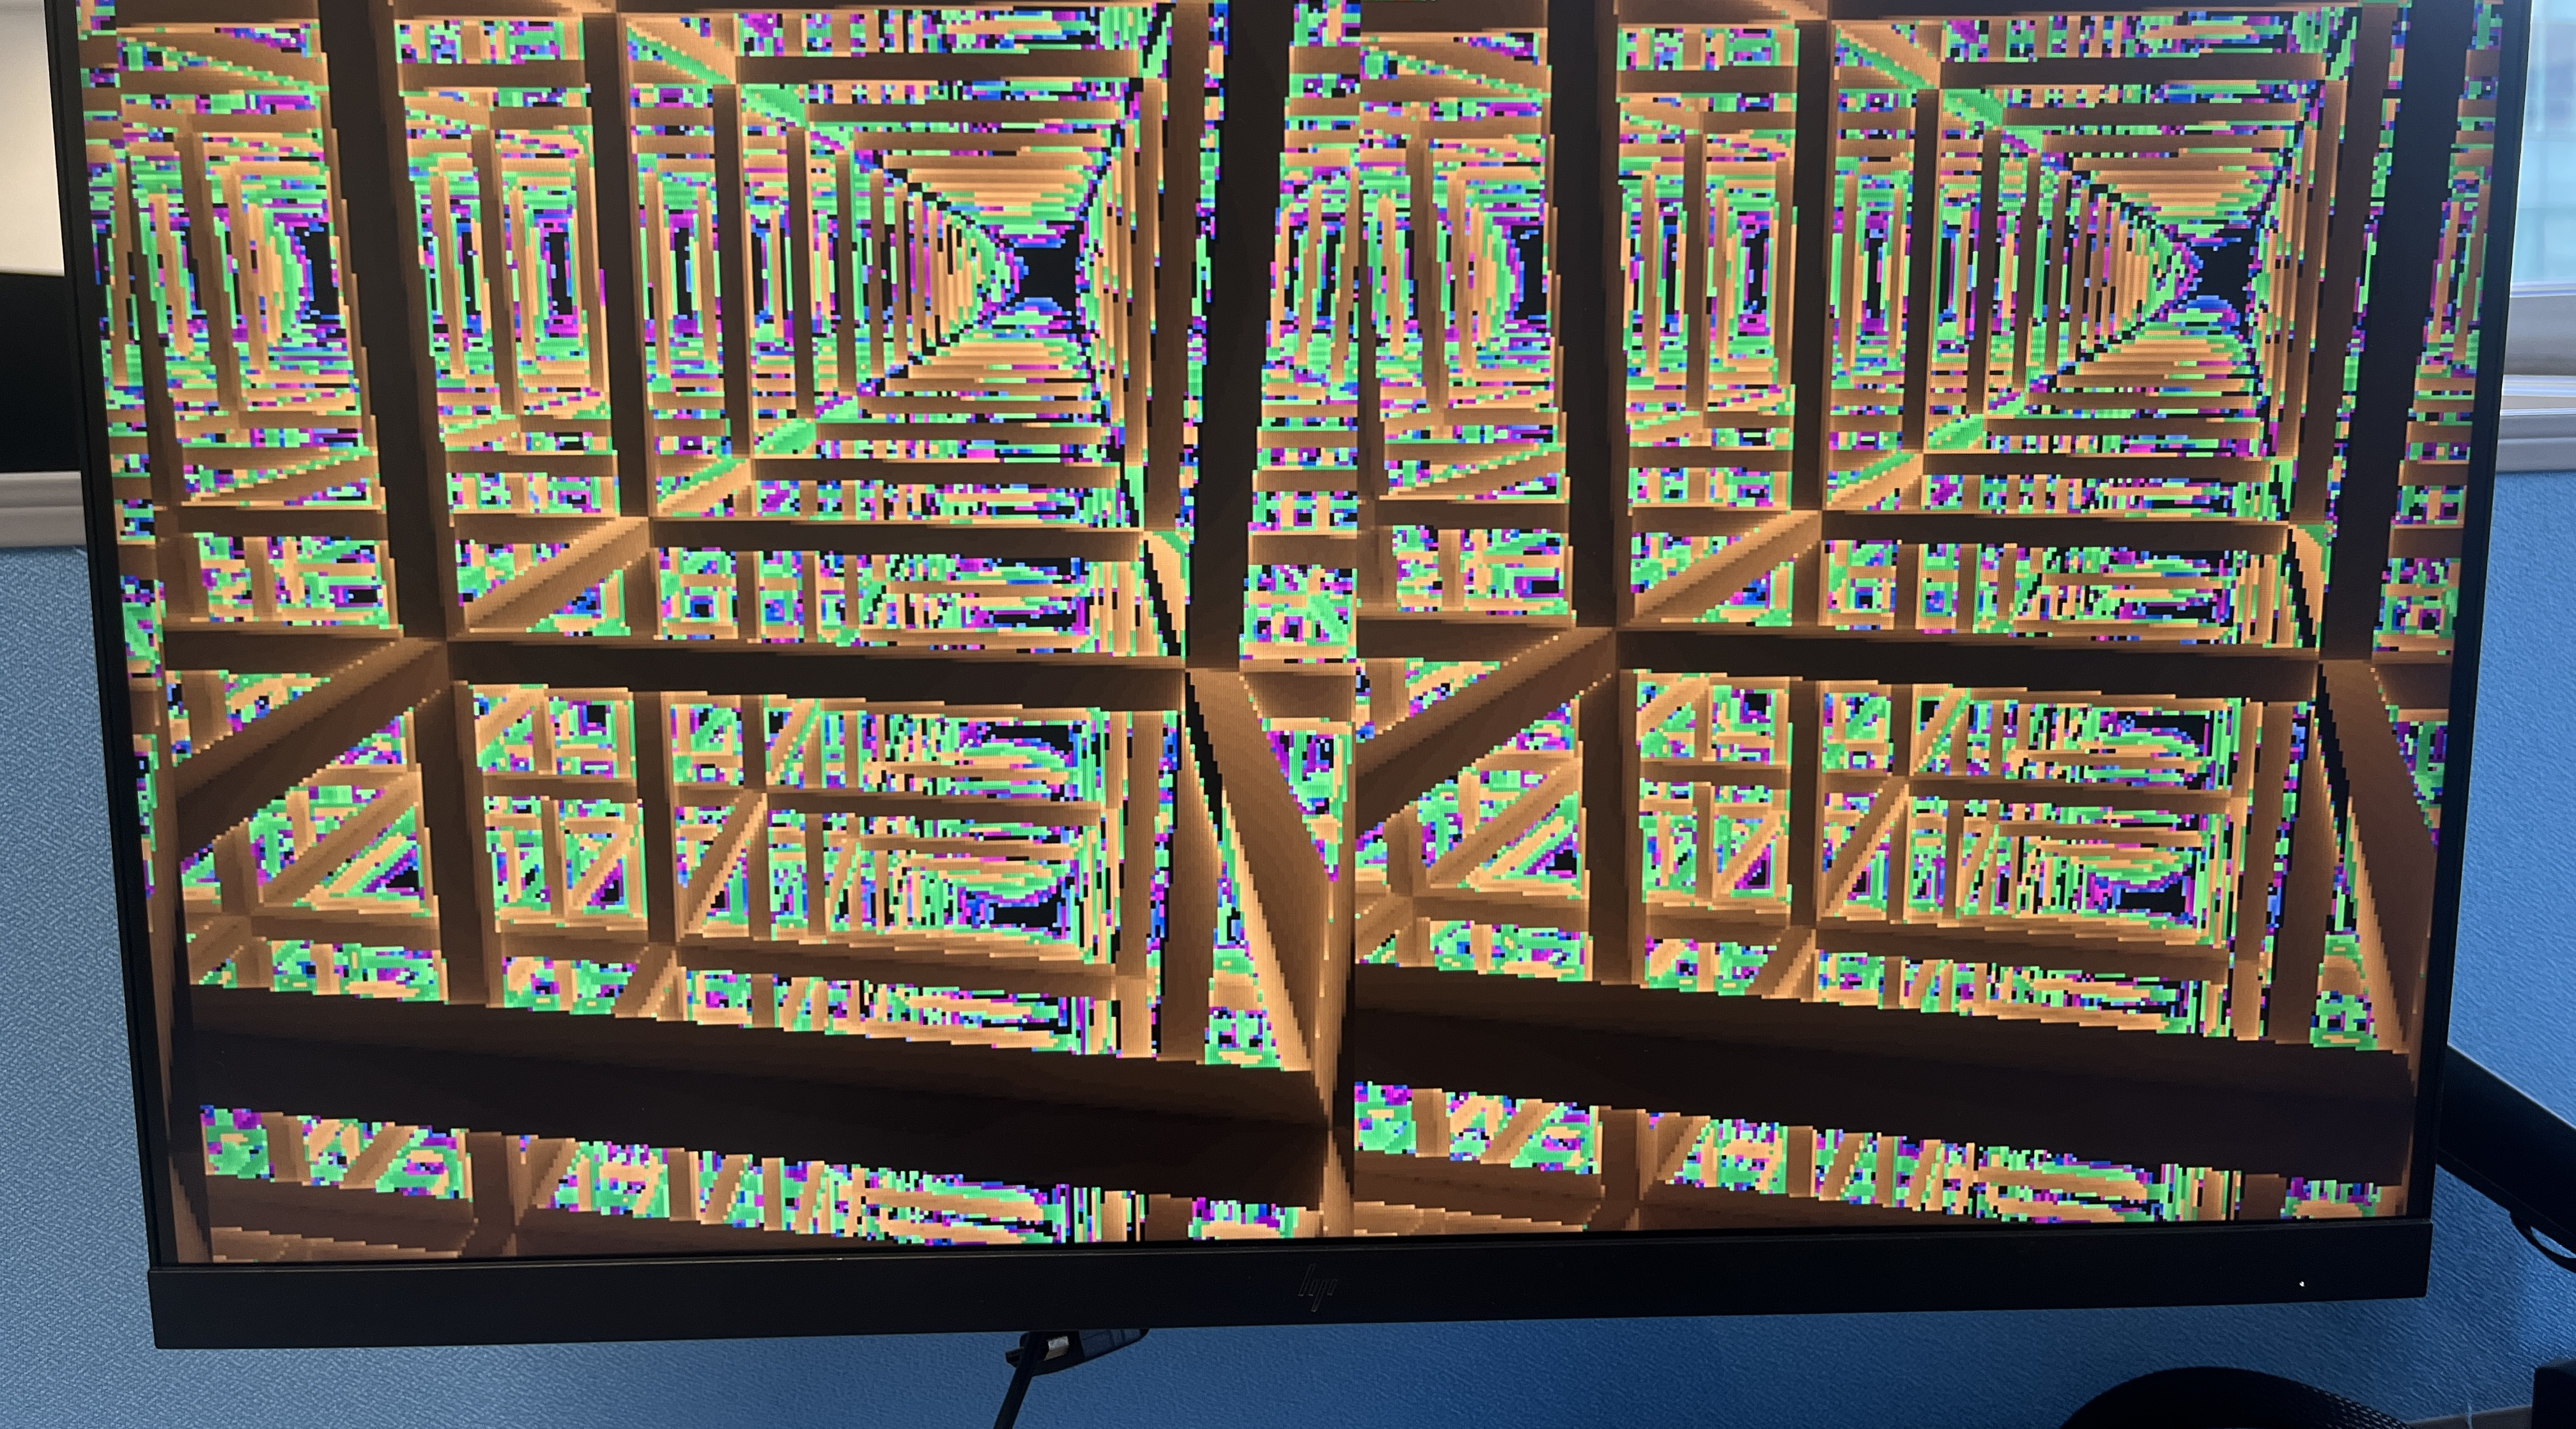
\includegraphics[width=\textwidth,height=0.28\textheight,keepaspectratio]{imgs/AppendixA/render_scaffold_tunnel_stereo.jpg}
    \caption{Scaffold tunnel, looking straight down a corridor. Iteration colourmap highlights infinite recession.}
\end{subfigure}

\vfill

\begin{subfigure}[b]{0.48\textwidth}
    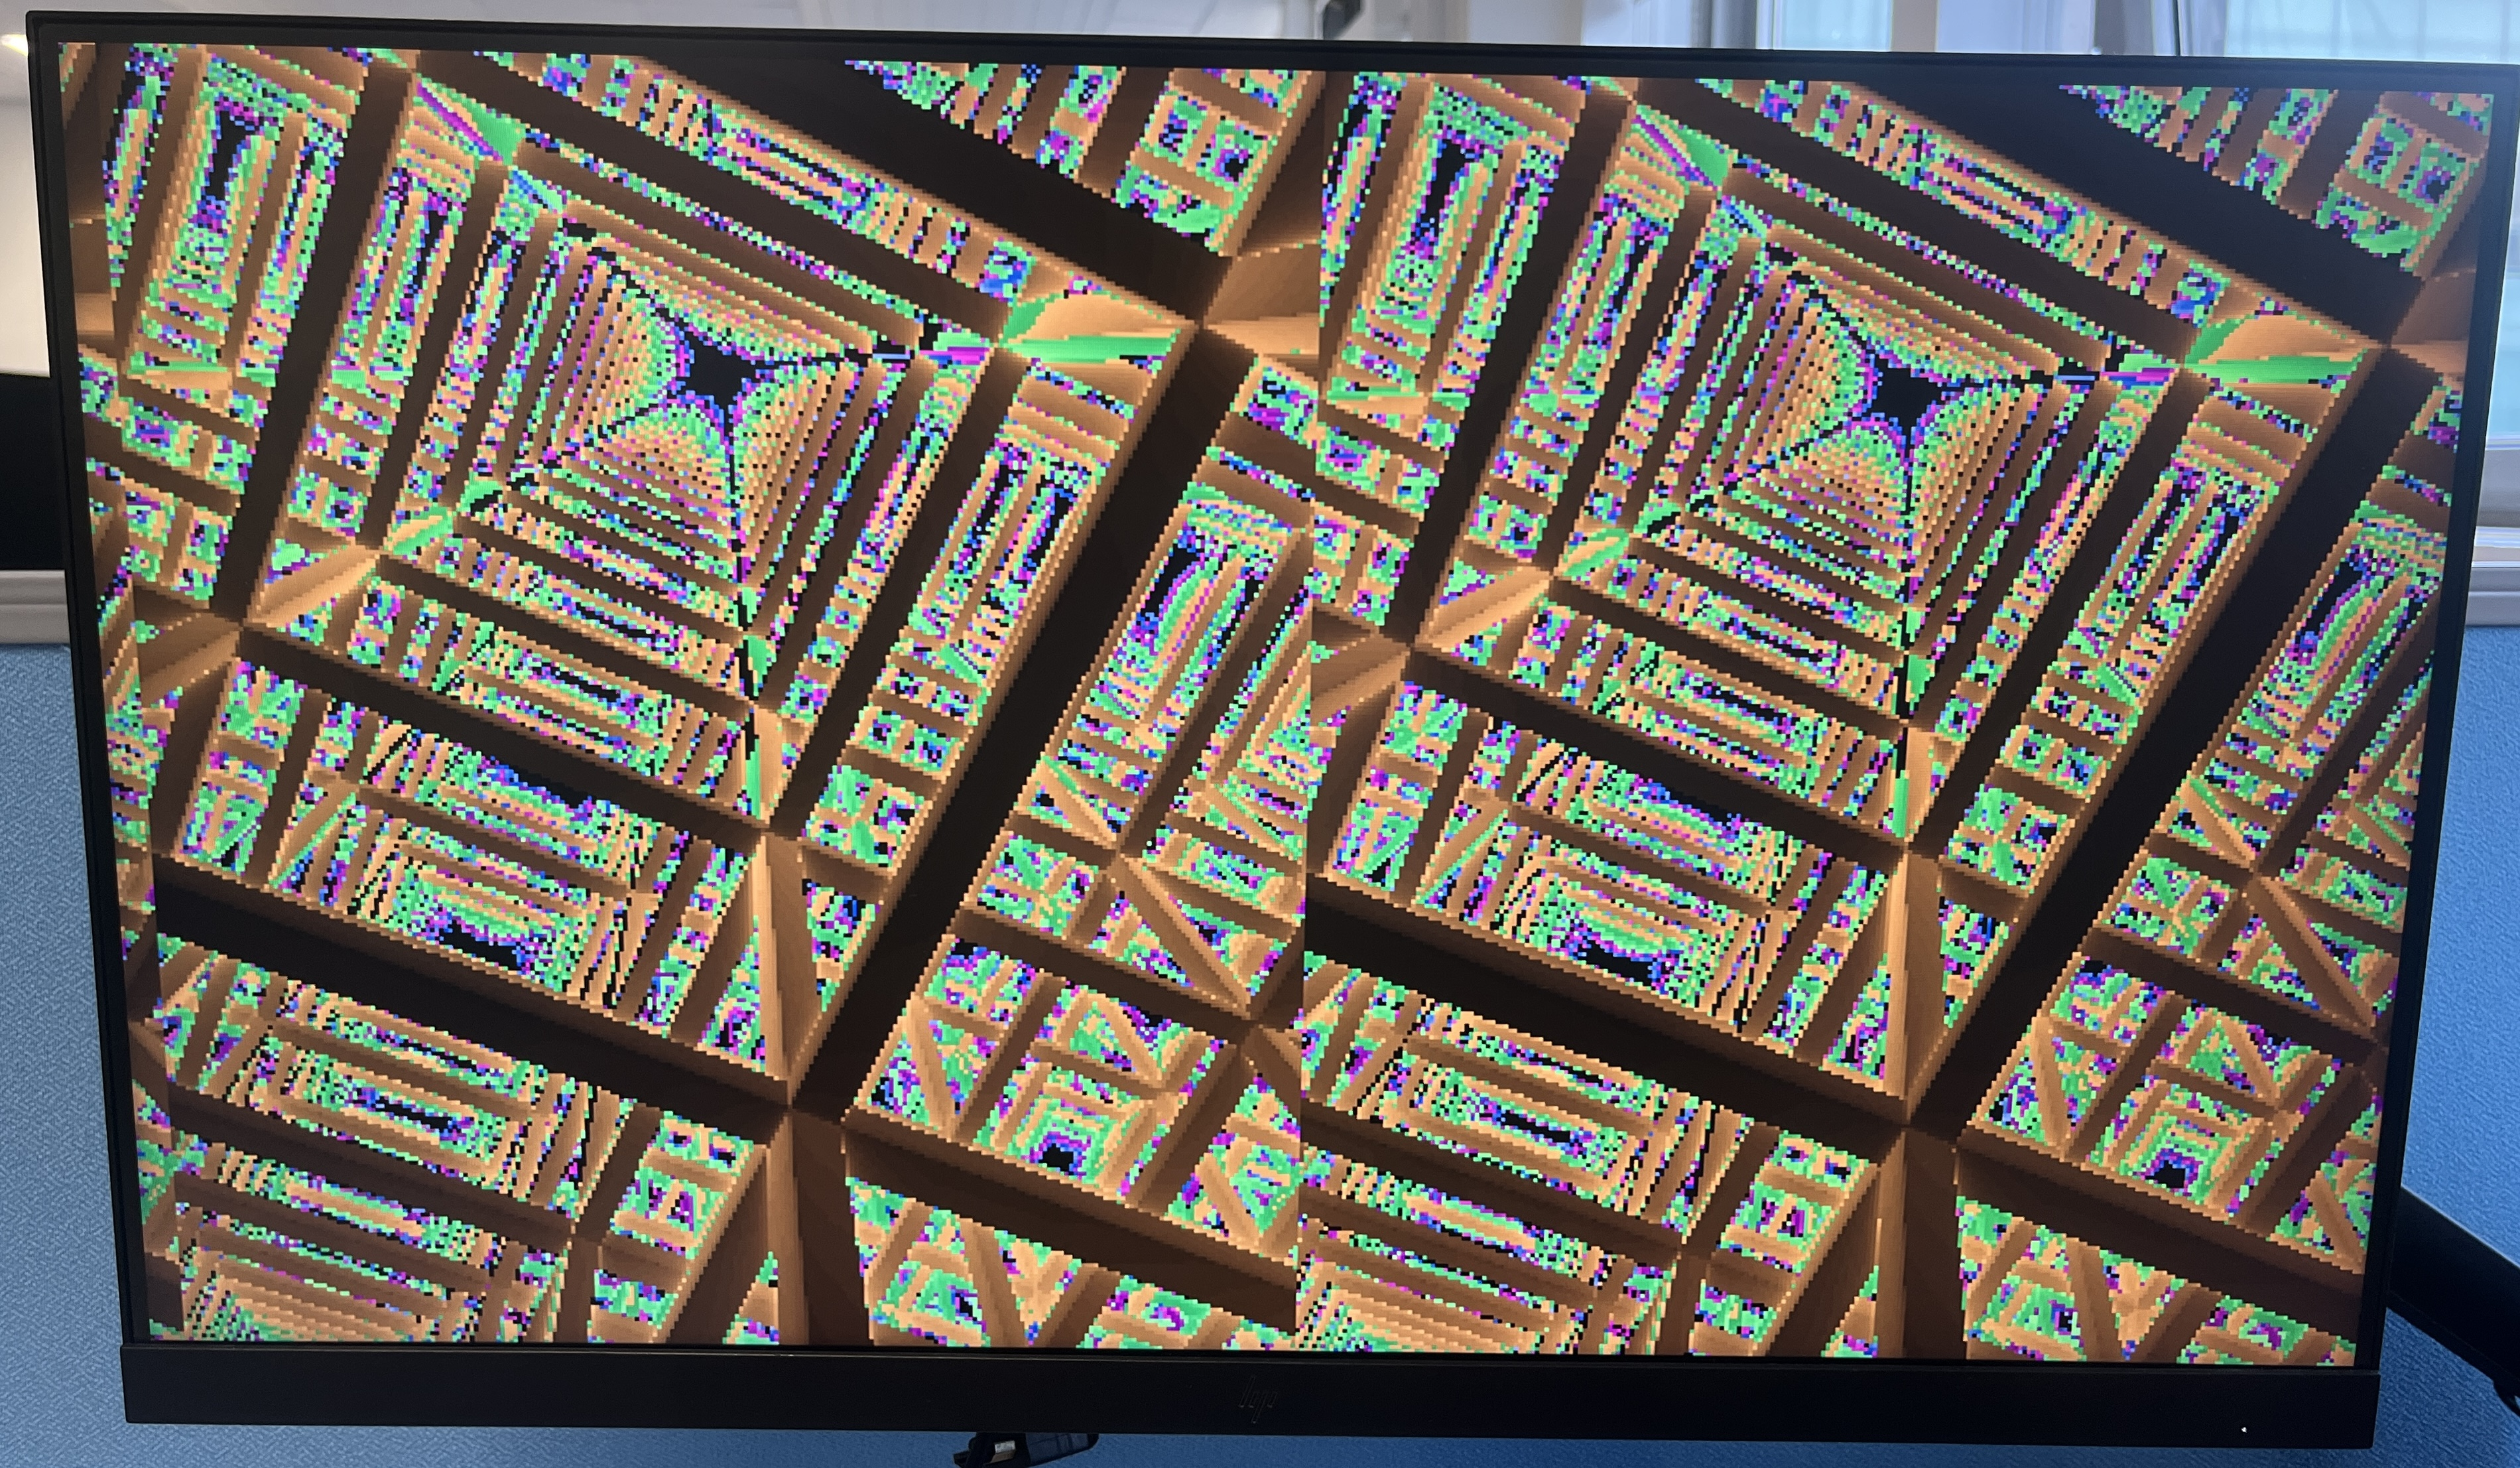
\includegraphics[width=\textwidth,height=0.28\textheight,keepaspectratio]{imgs/AppendixA/render_scaffold_zenith_stereo.jpg}
    \caption{Scaffold zenith view: camera looking straight up through nested box frames into infinite depth.}
\end{subfigure}\hfill
\begin{subfigure}[b]{0.48\textwidth}
    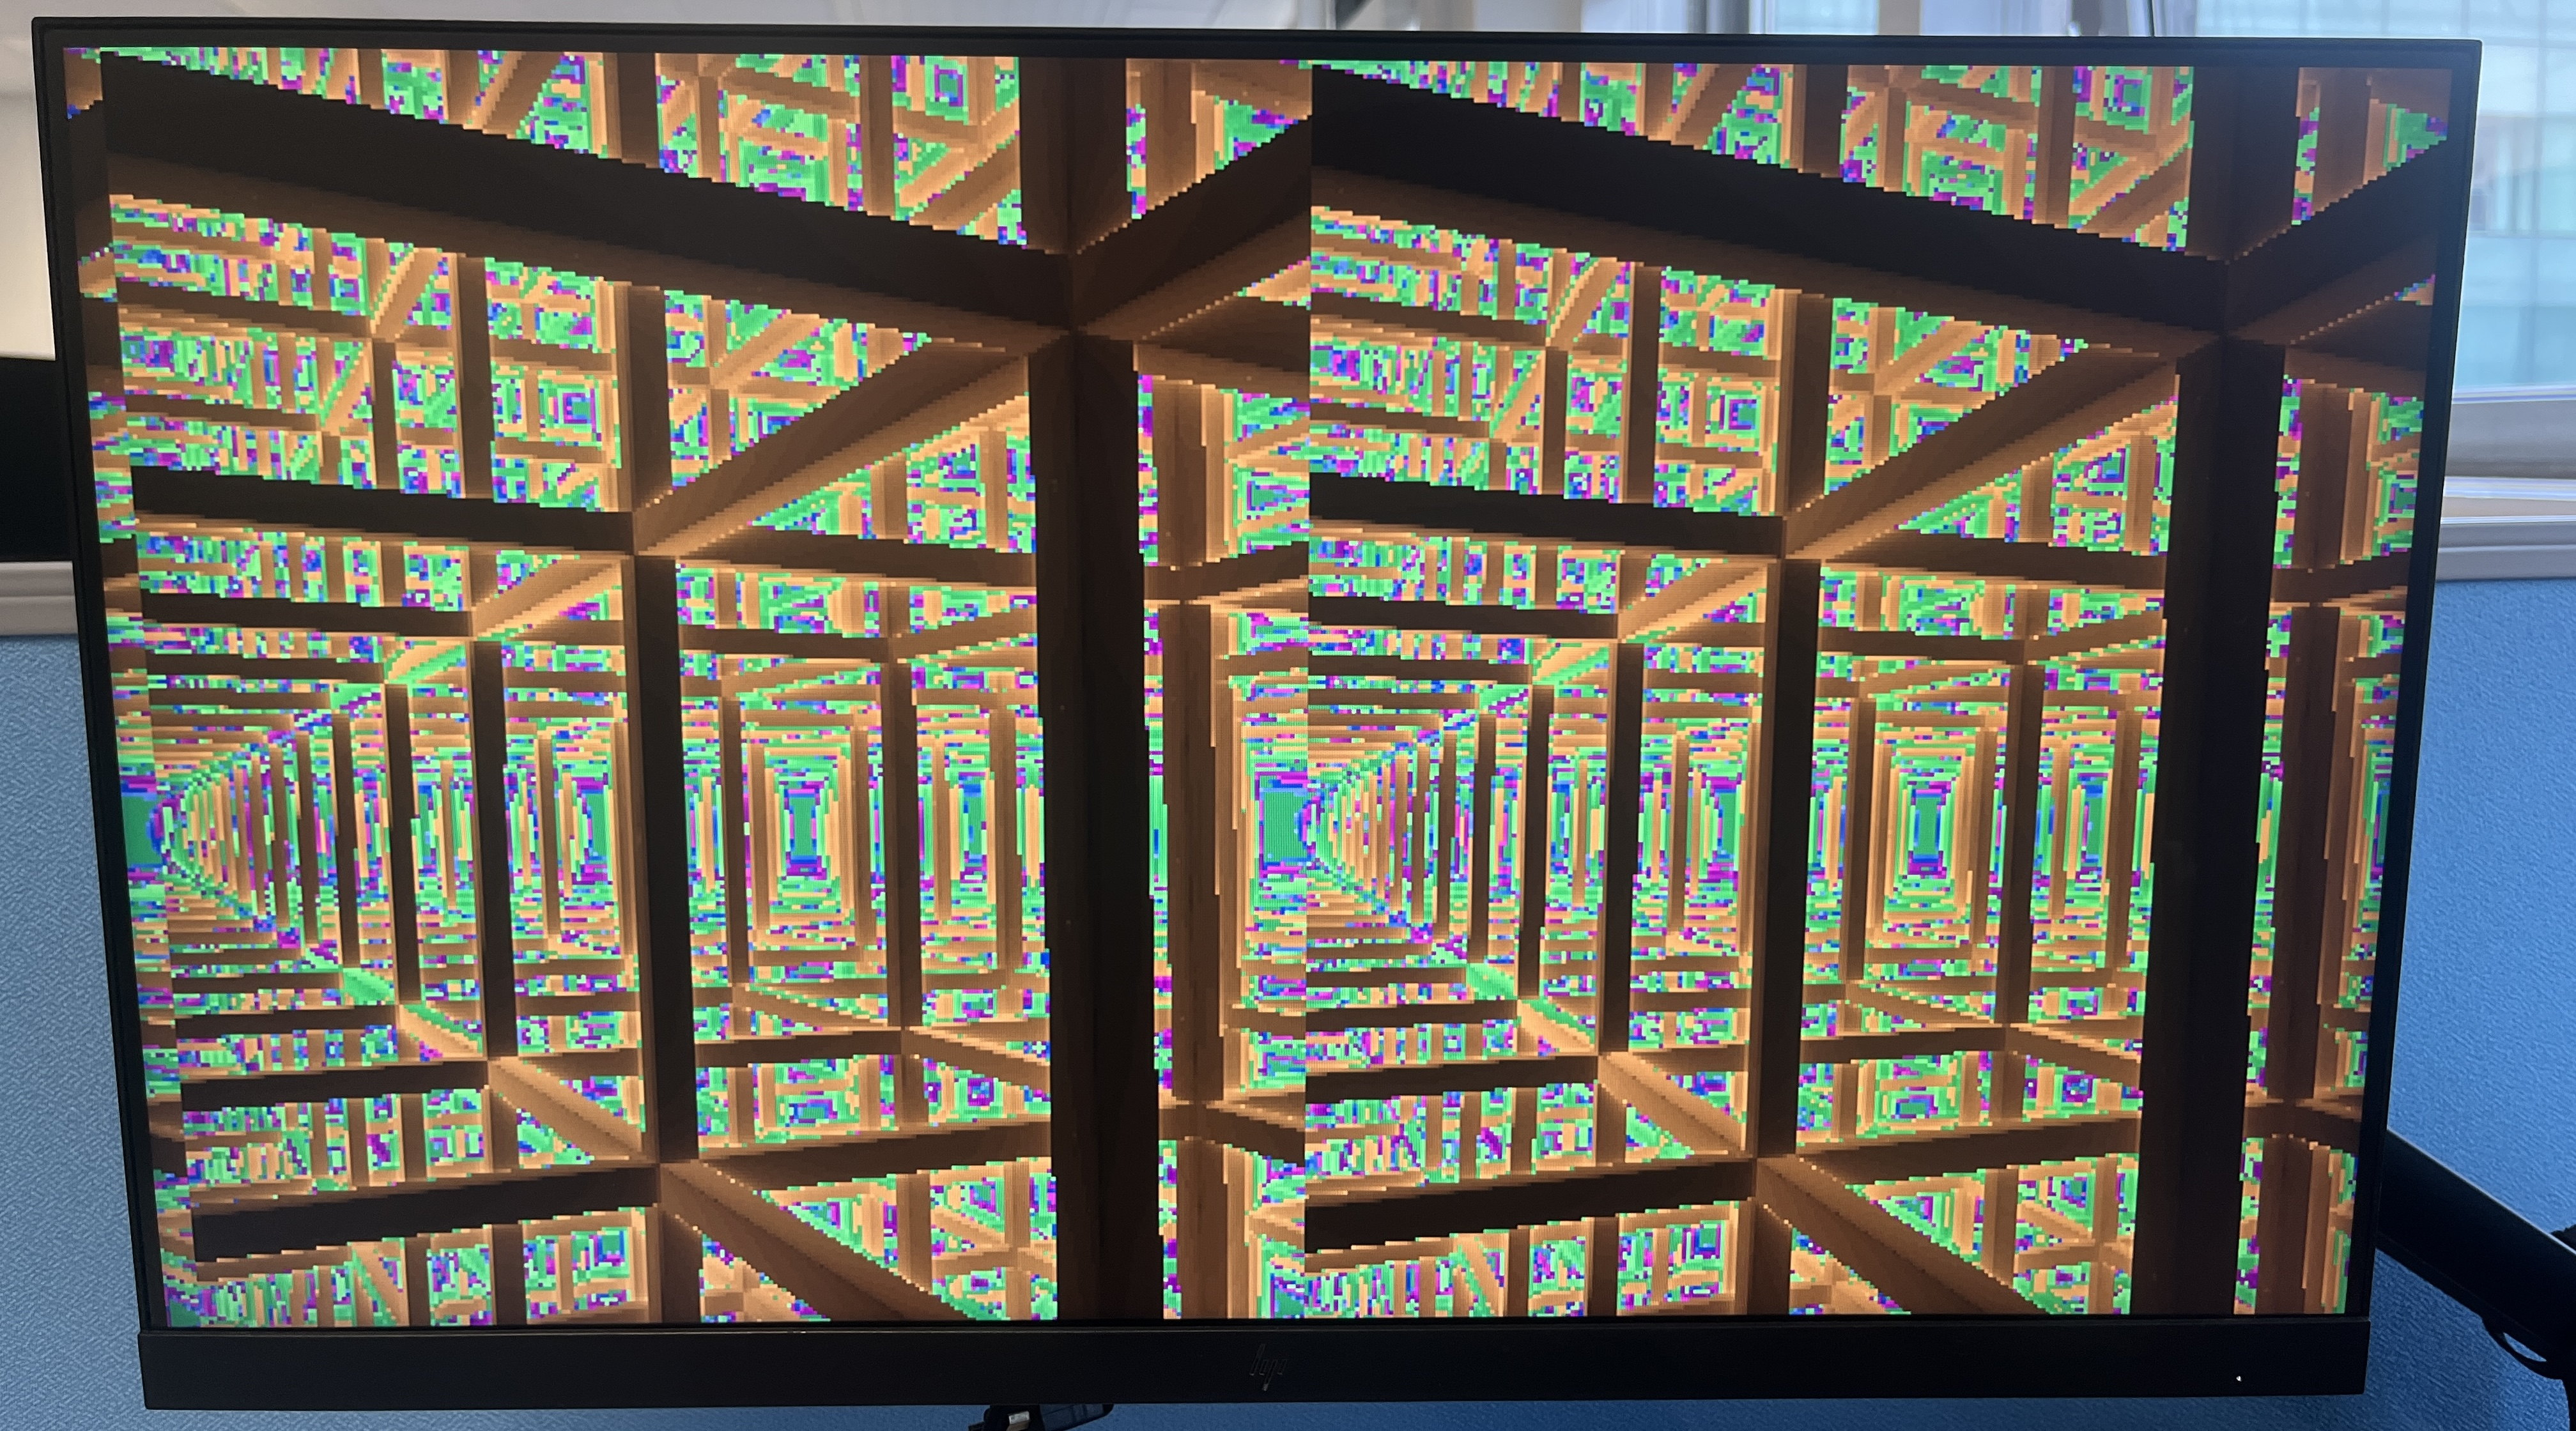
\includegraphics[width=\textwidth,height=0.28\textheight,keepaspectratio]{imgs/AppendixA/render_scaffold_corridor_stereo.jpg}
    \caption{Scaffold corridor, angled stereo shot. Space repetition cell boundaries clearly delineated.}
\end{subfigure}

\vfill

\begin{subfigure}[b]{0.48\textwidth}
    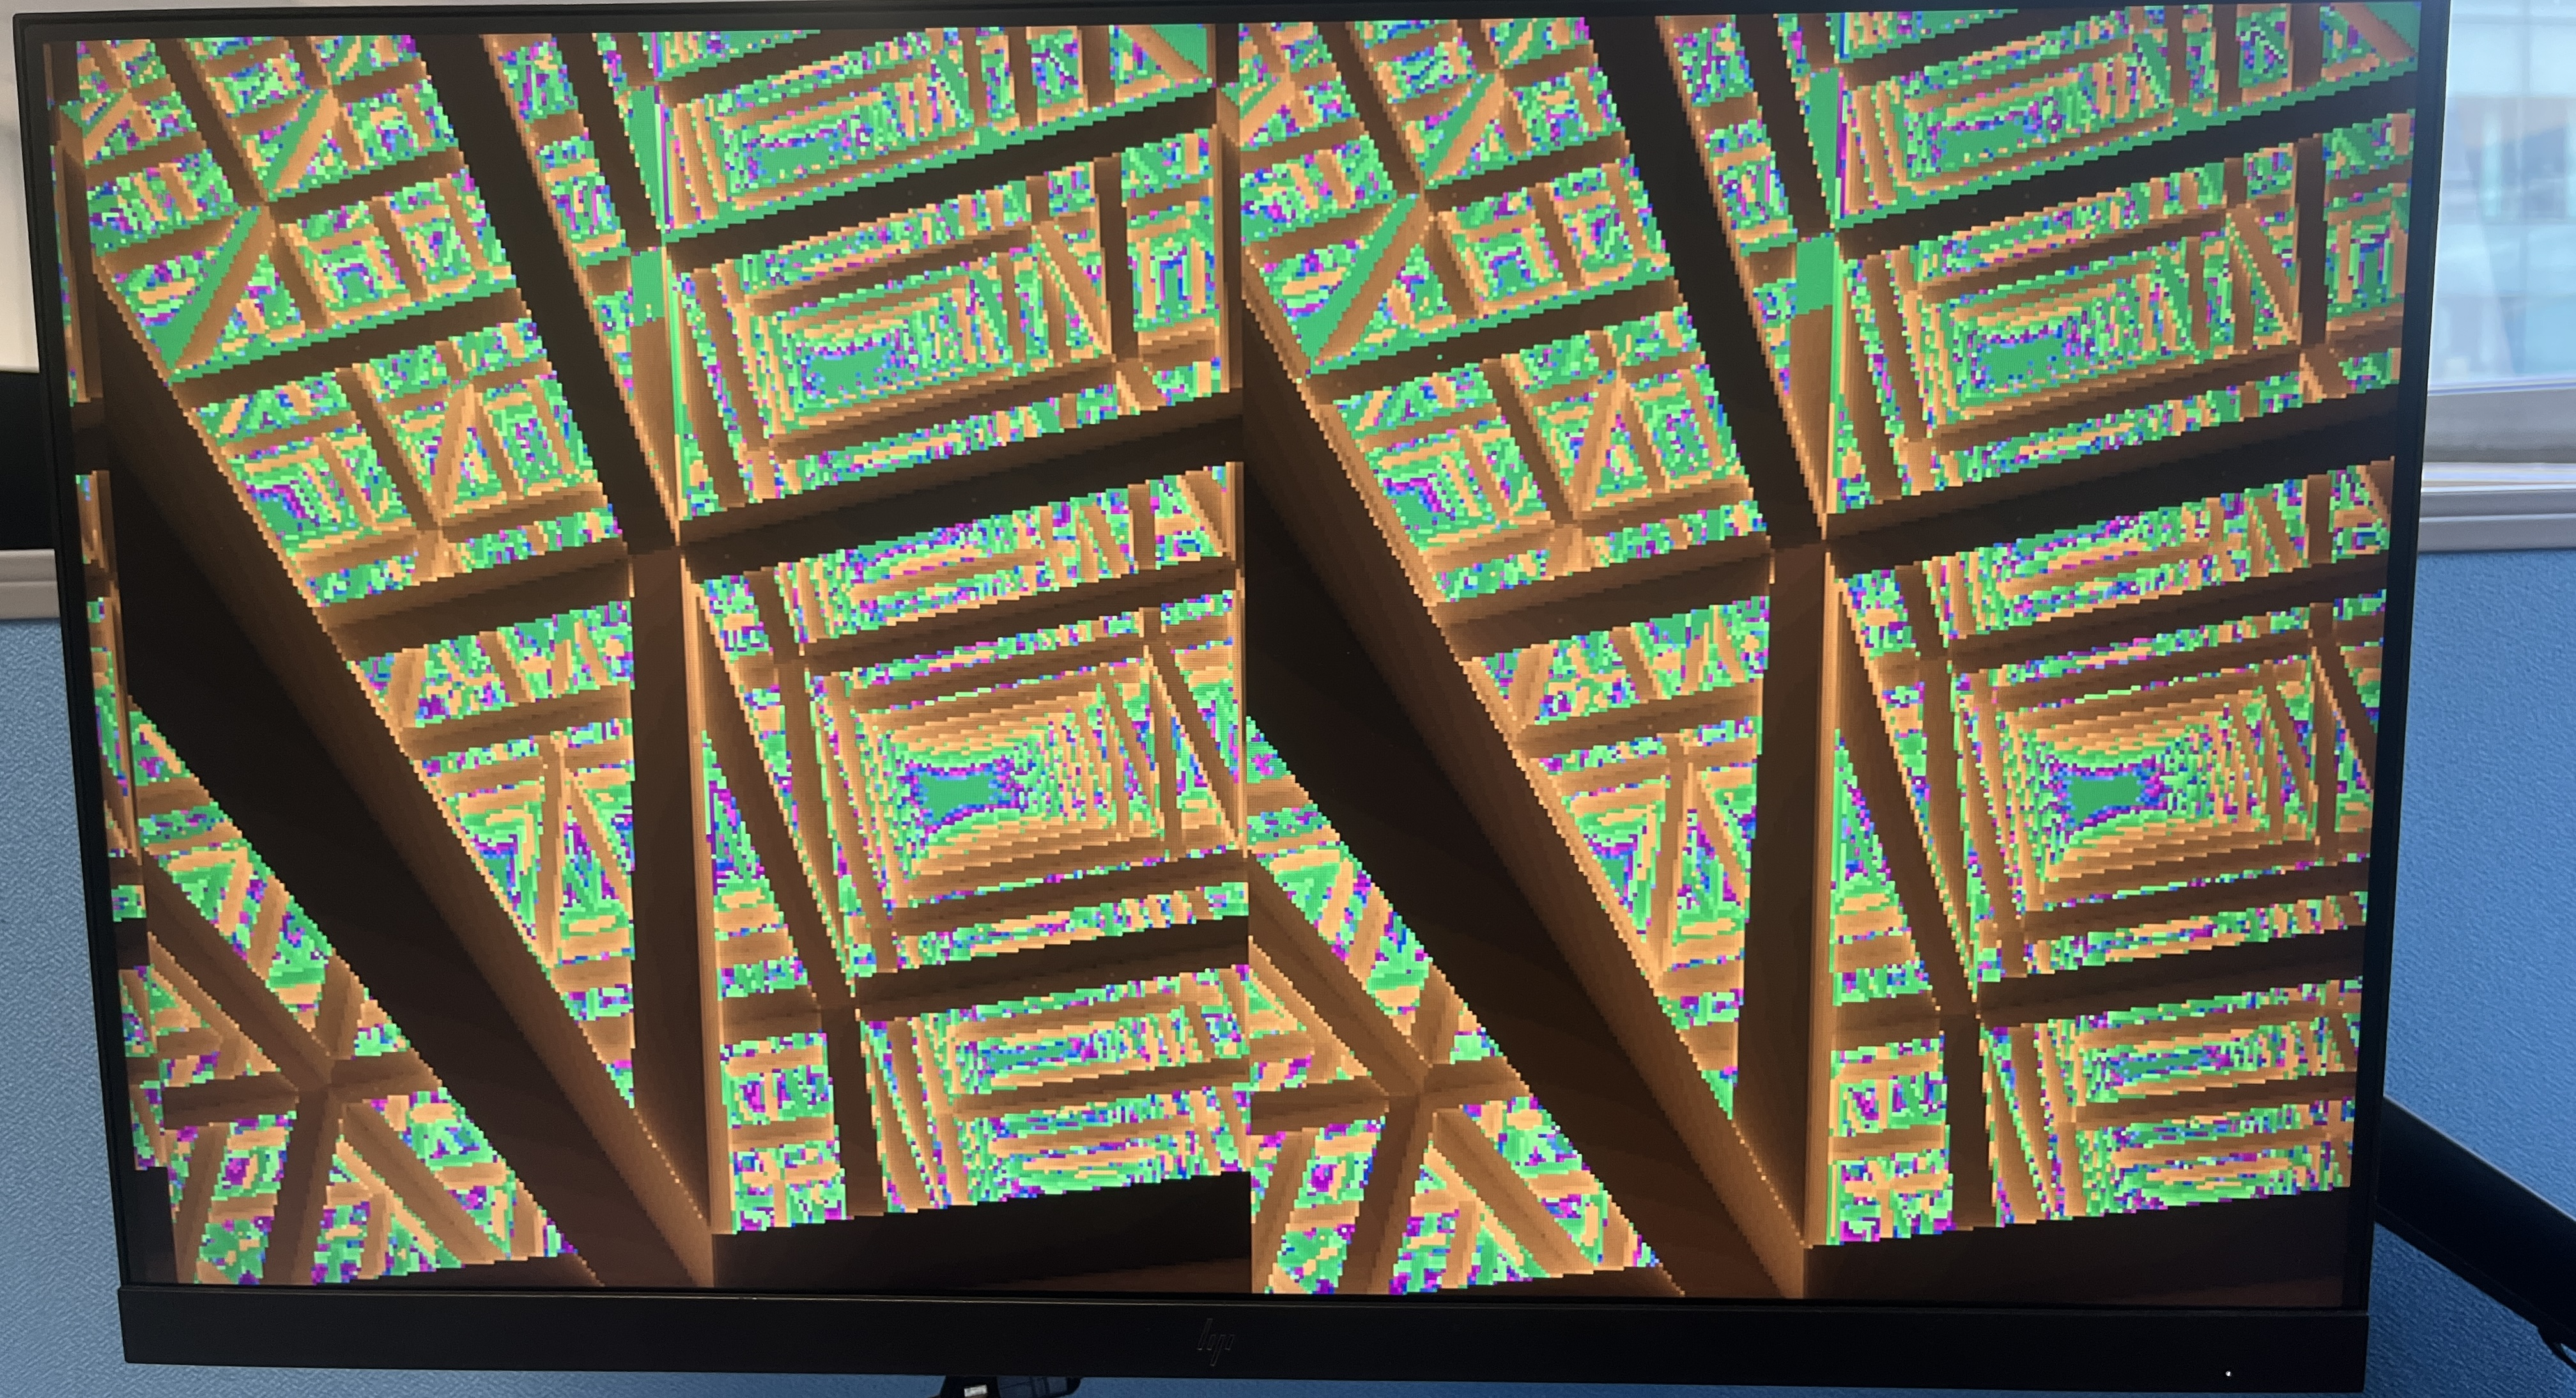
\includegraphics[width=\textwidth,height=0.28\textheight,keepaspectratio]{imgs/AppendixA/render_scaffold_diagonal_stereo.jpg}
    \caption{Scaffold diagonal view, close to the frame geometry. FP27 precision resolves fine strut edges without aliasing.}
\end{subfigure}\hfill
\begin{subfigure}[b]{0.48\textwidth}
    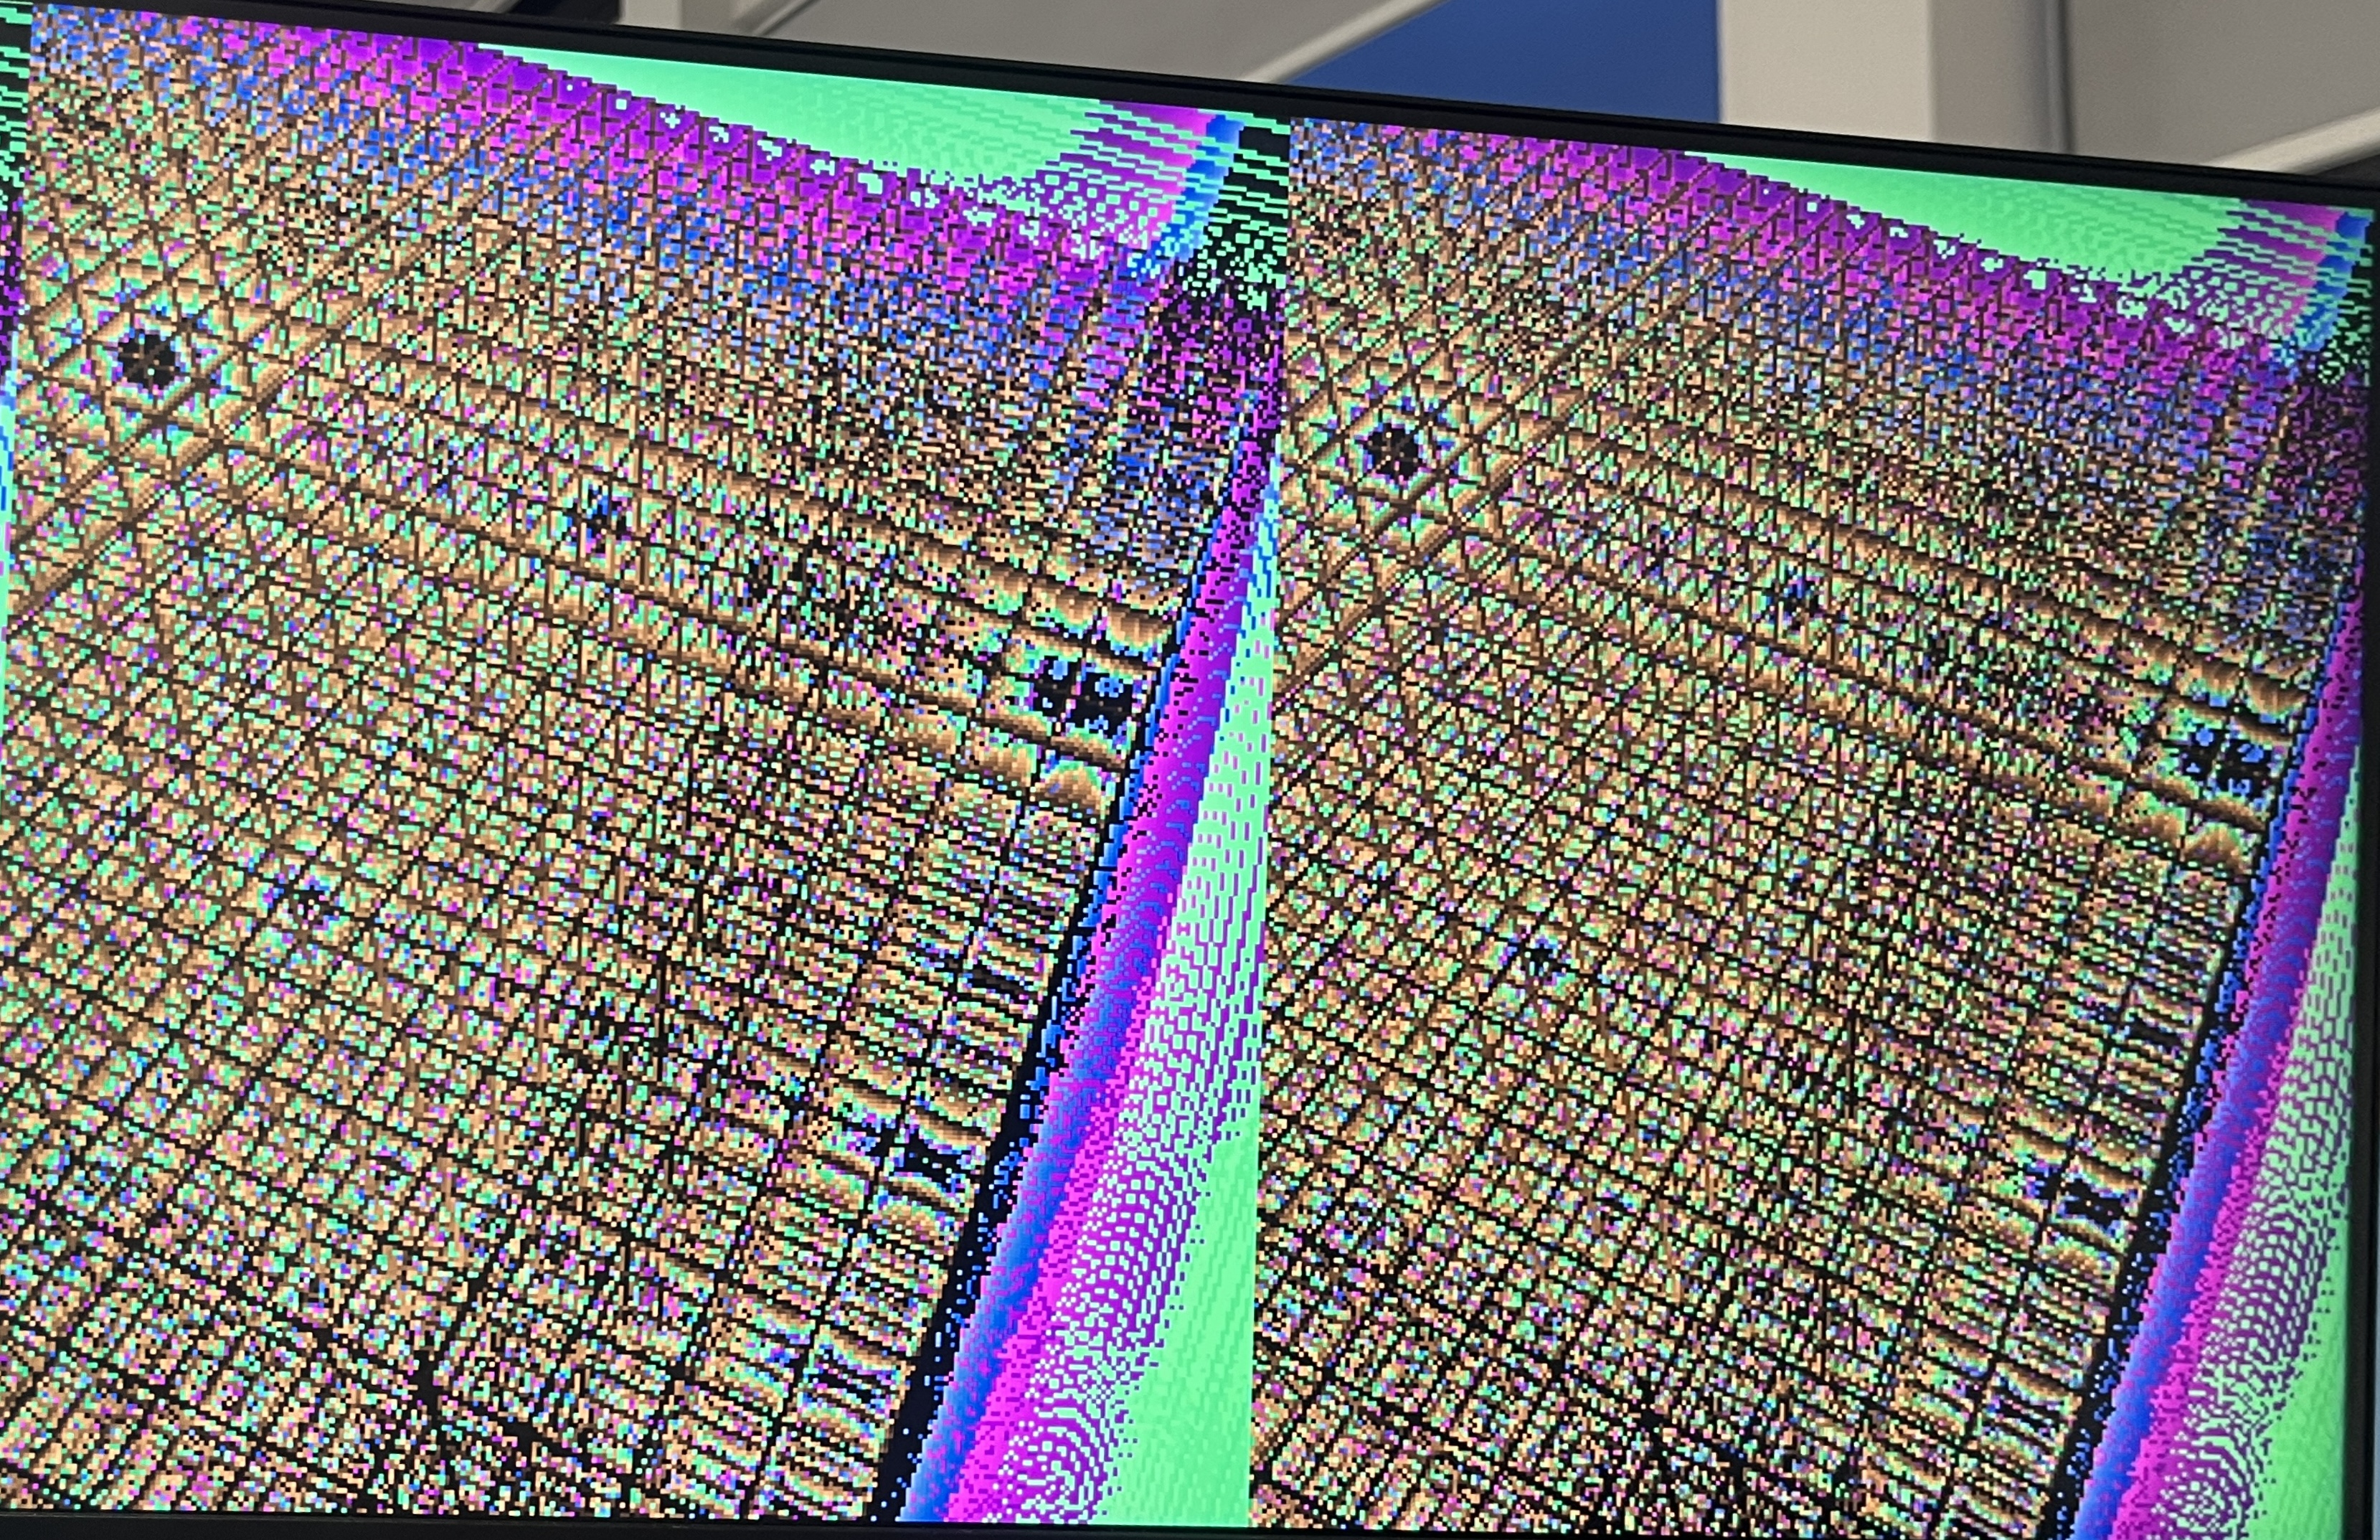
\includegraphics[width=\textwidth,height=0.28\textheight,keepaspectratio]{imgs/AppendixA/headset_photo_2.jpg}
    \caption{Assembled VR headset, side profile. Quest~2 headstrap adapter and 90-degree HDMI cable routing visible.}
\end{subfigure}
\caption{Stereoscopic render gallery III, scaffold scene perspectives on physical board.}
\end{figure}

\clearpage

% ----------------------------------------------------------------
%  Page 4 — GLSL software reference renders: scaffold interior views
% ----------------------------------------------------------------
\begin{figure}[H]
\vspace*{-0.5cm}
\centering
\begin{subfigure}[b]{0.48\textwidth}
    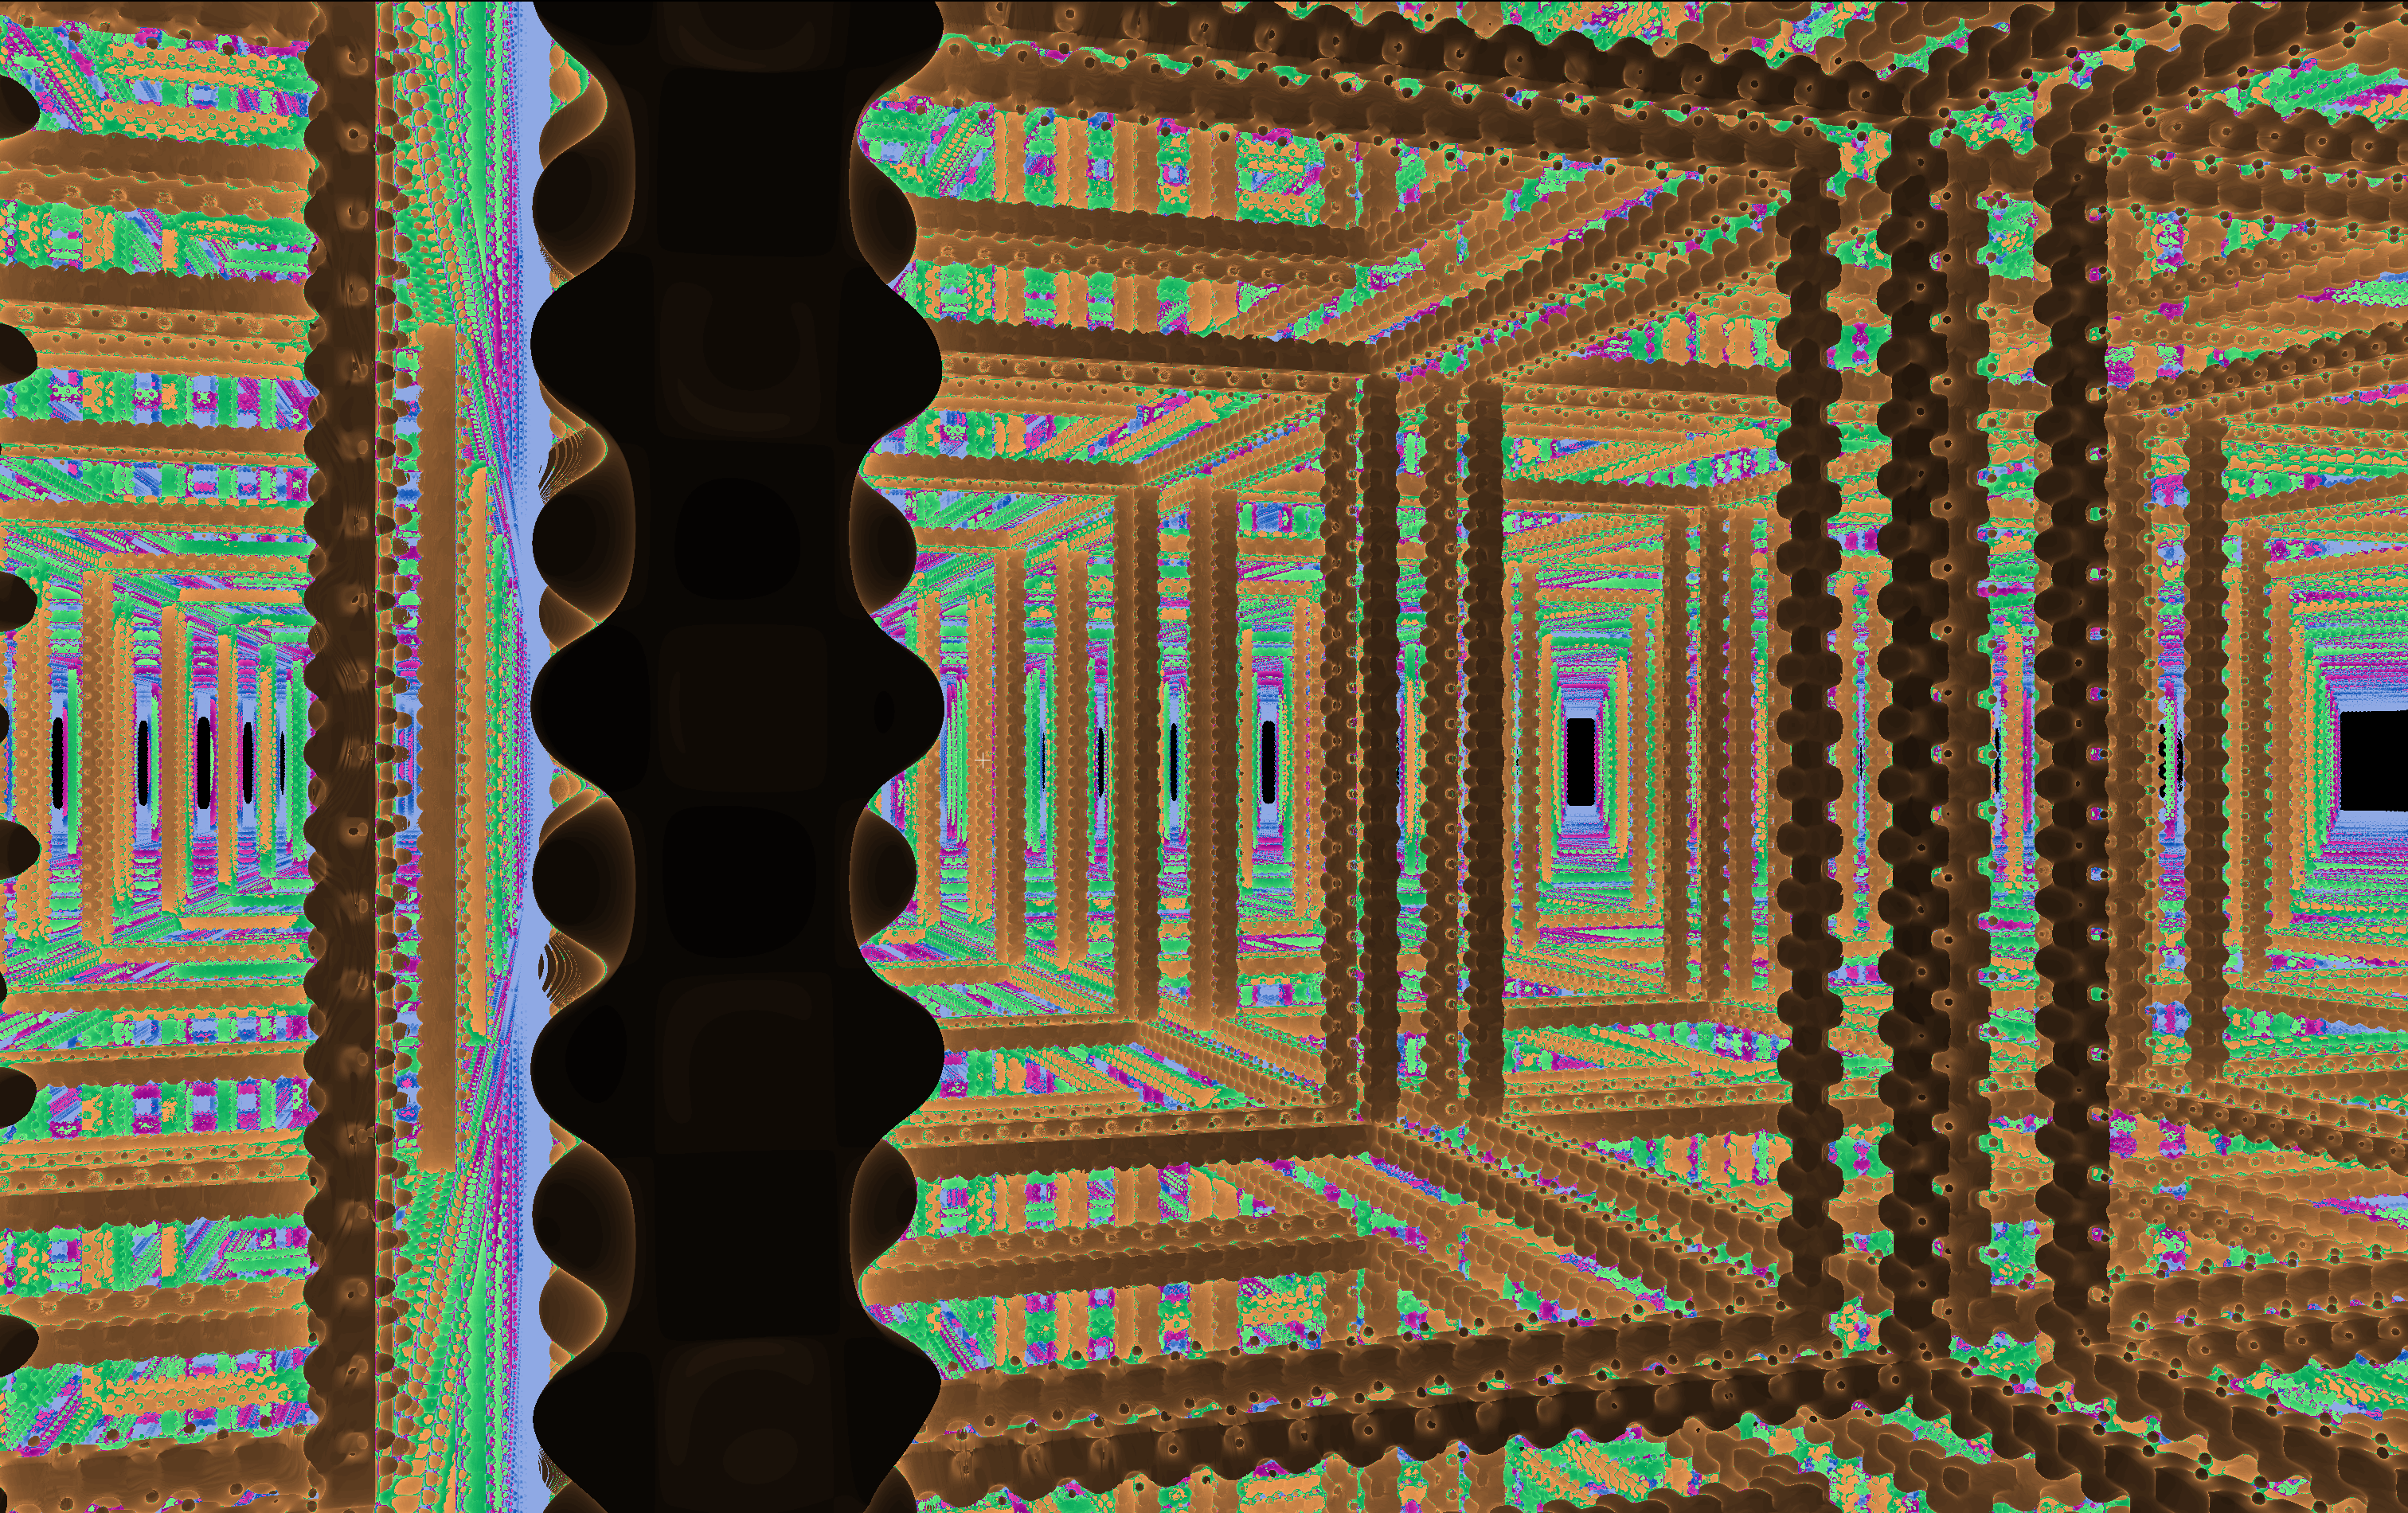
\includegraphics[width=\textwidth,height=0.28\textheight,keepaspectratio]{imgs/AppendixA/render_scaffold_glsl_pillar.png}
    \caption{GLSL reference renderer, scaffold interior with twisted strut column in foreground, infinite depth field.}
\end{subfigure}\hfill
\begin{subfigure}[b]{0.48\textwidth}
    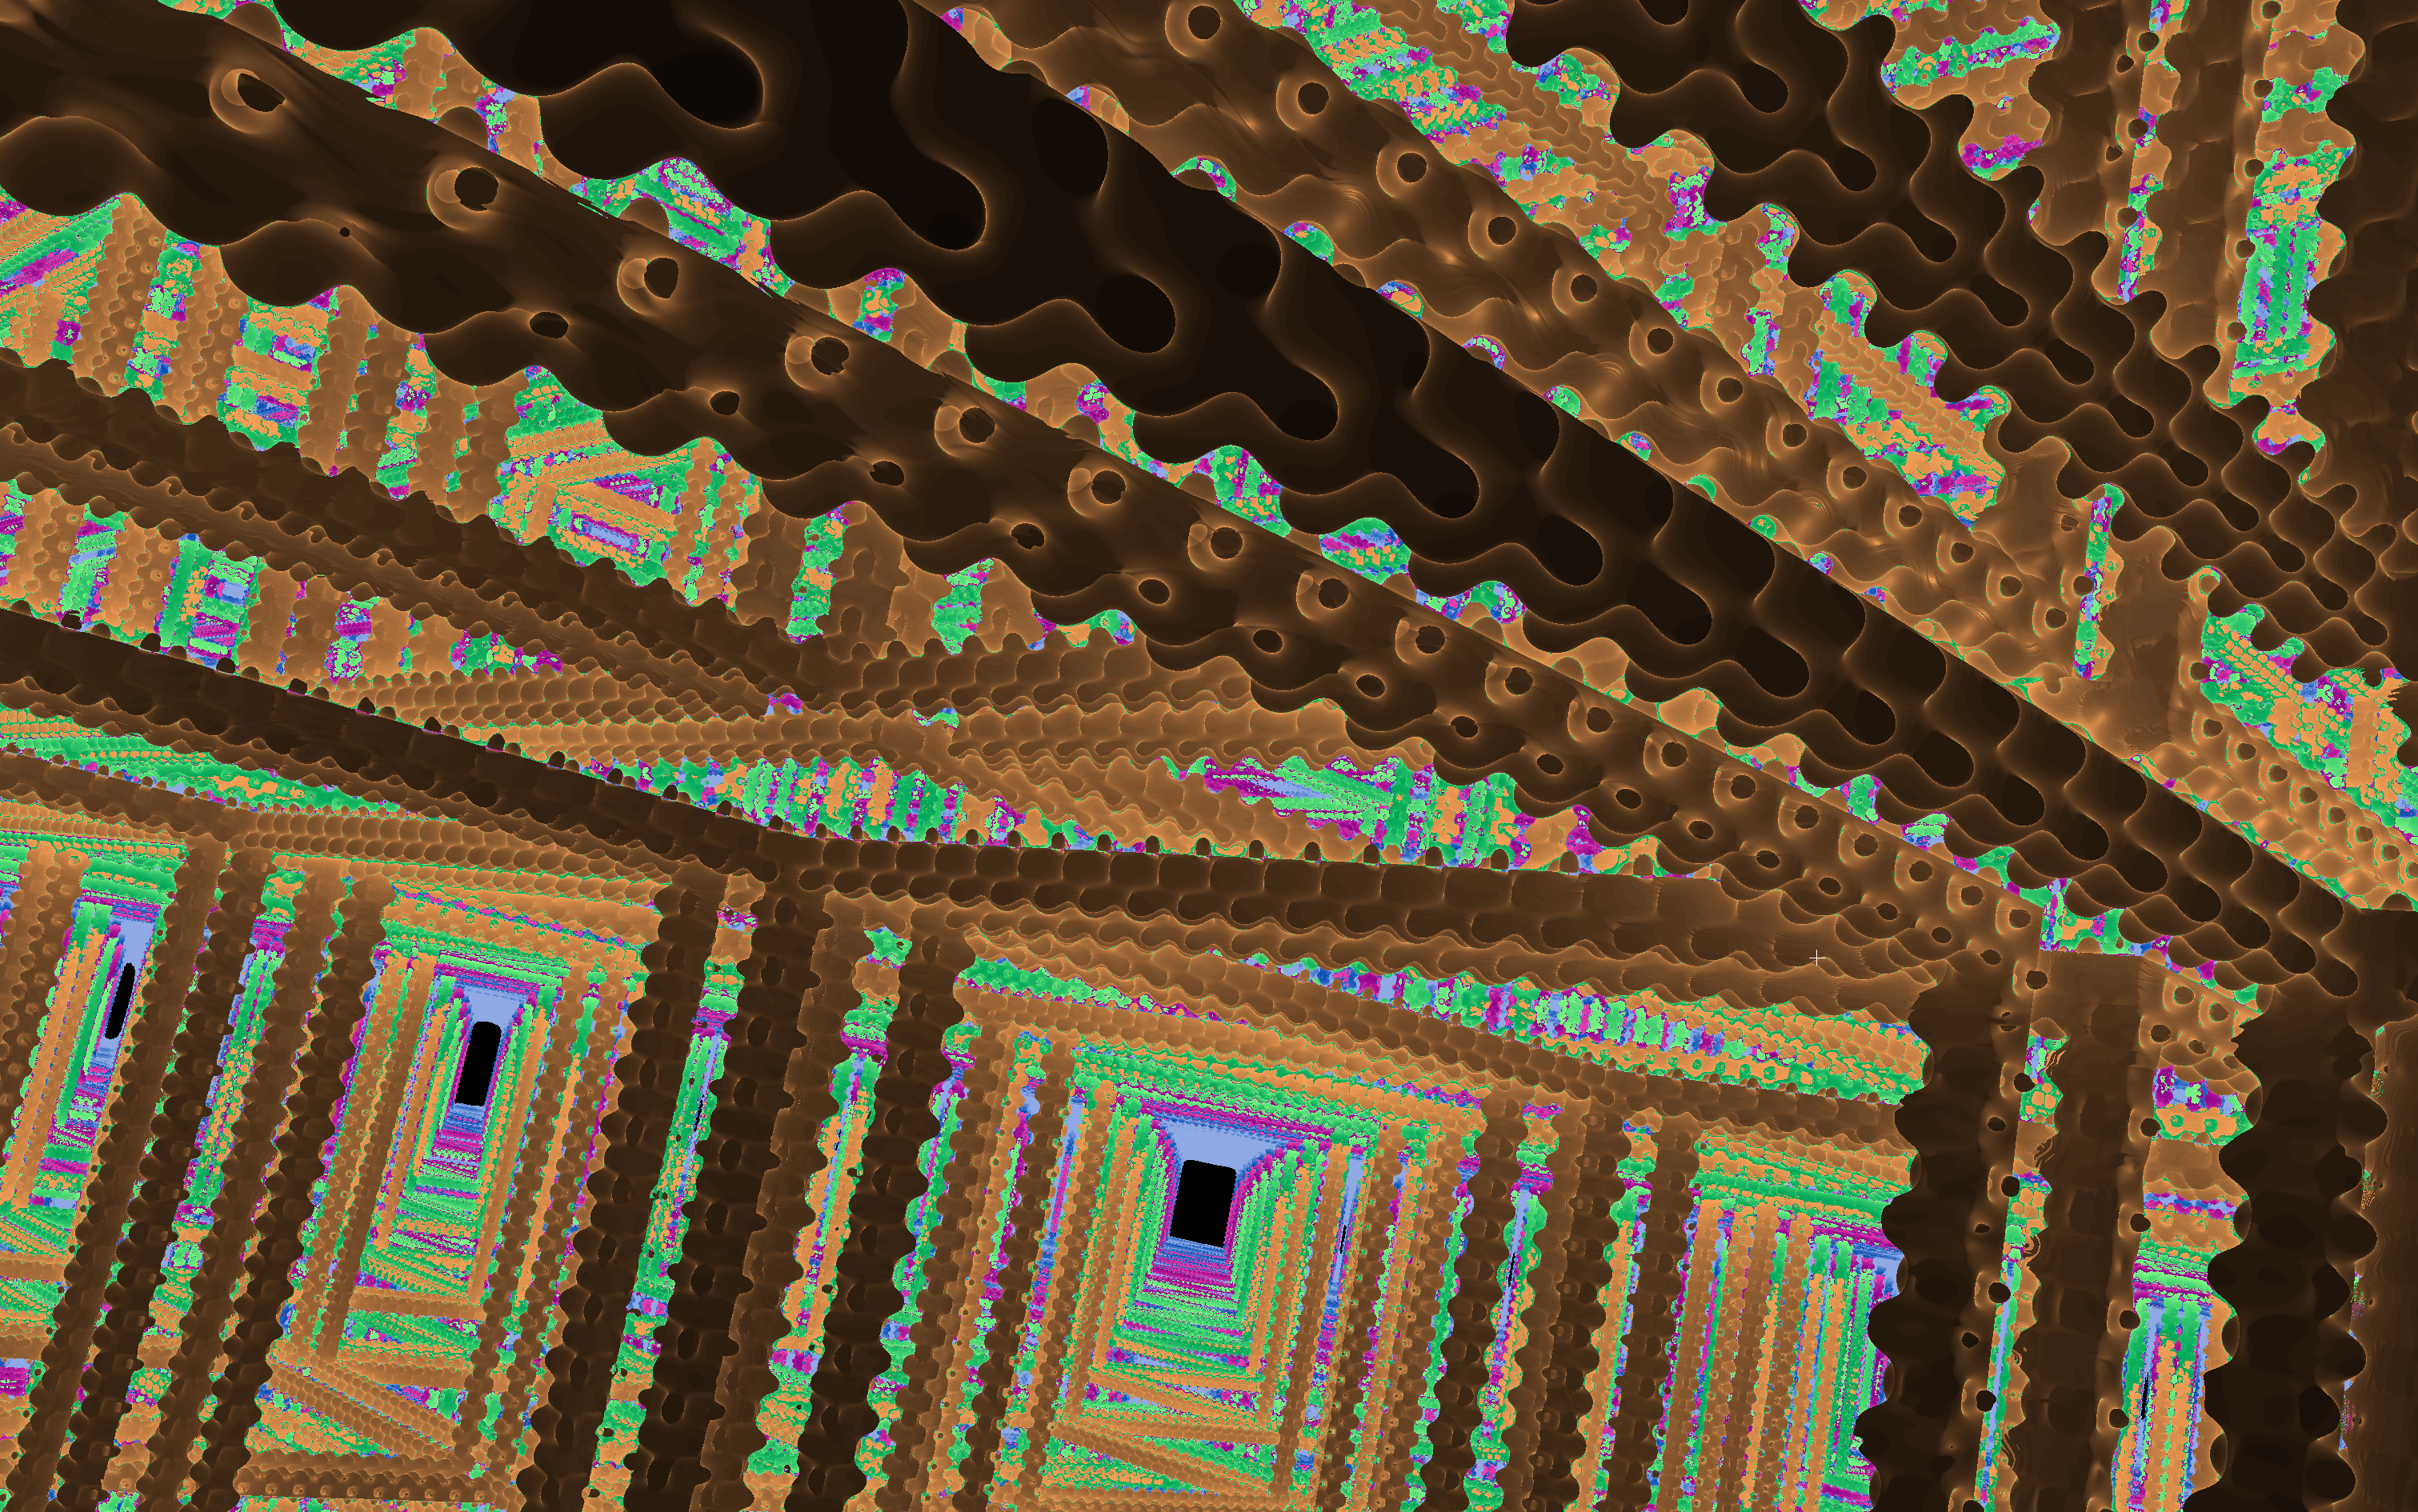
\includegraphics[width=\textwidth,height=0.28\textheight,keepaspectratio]{imgs/AppendixA/render_scaffold_glsl_ceiling.png}
    \caption{GLSL scaffold ceiling close-up. Honeycomb-textured surface on the box-frame boundary under ambient light.}
\end{subfigure}

\vfill

\begin{subfigure}[b]{0.48\textwidth}
    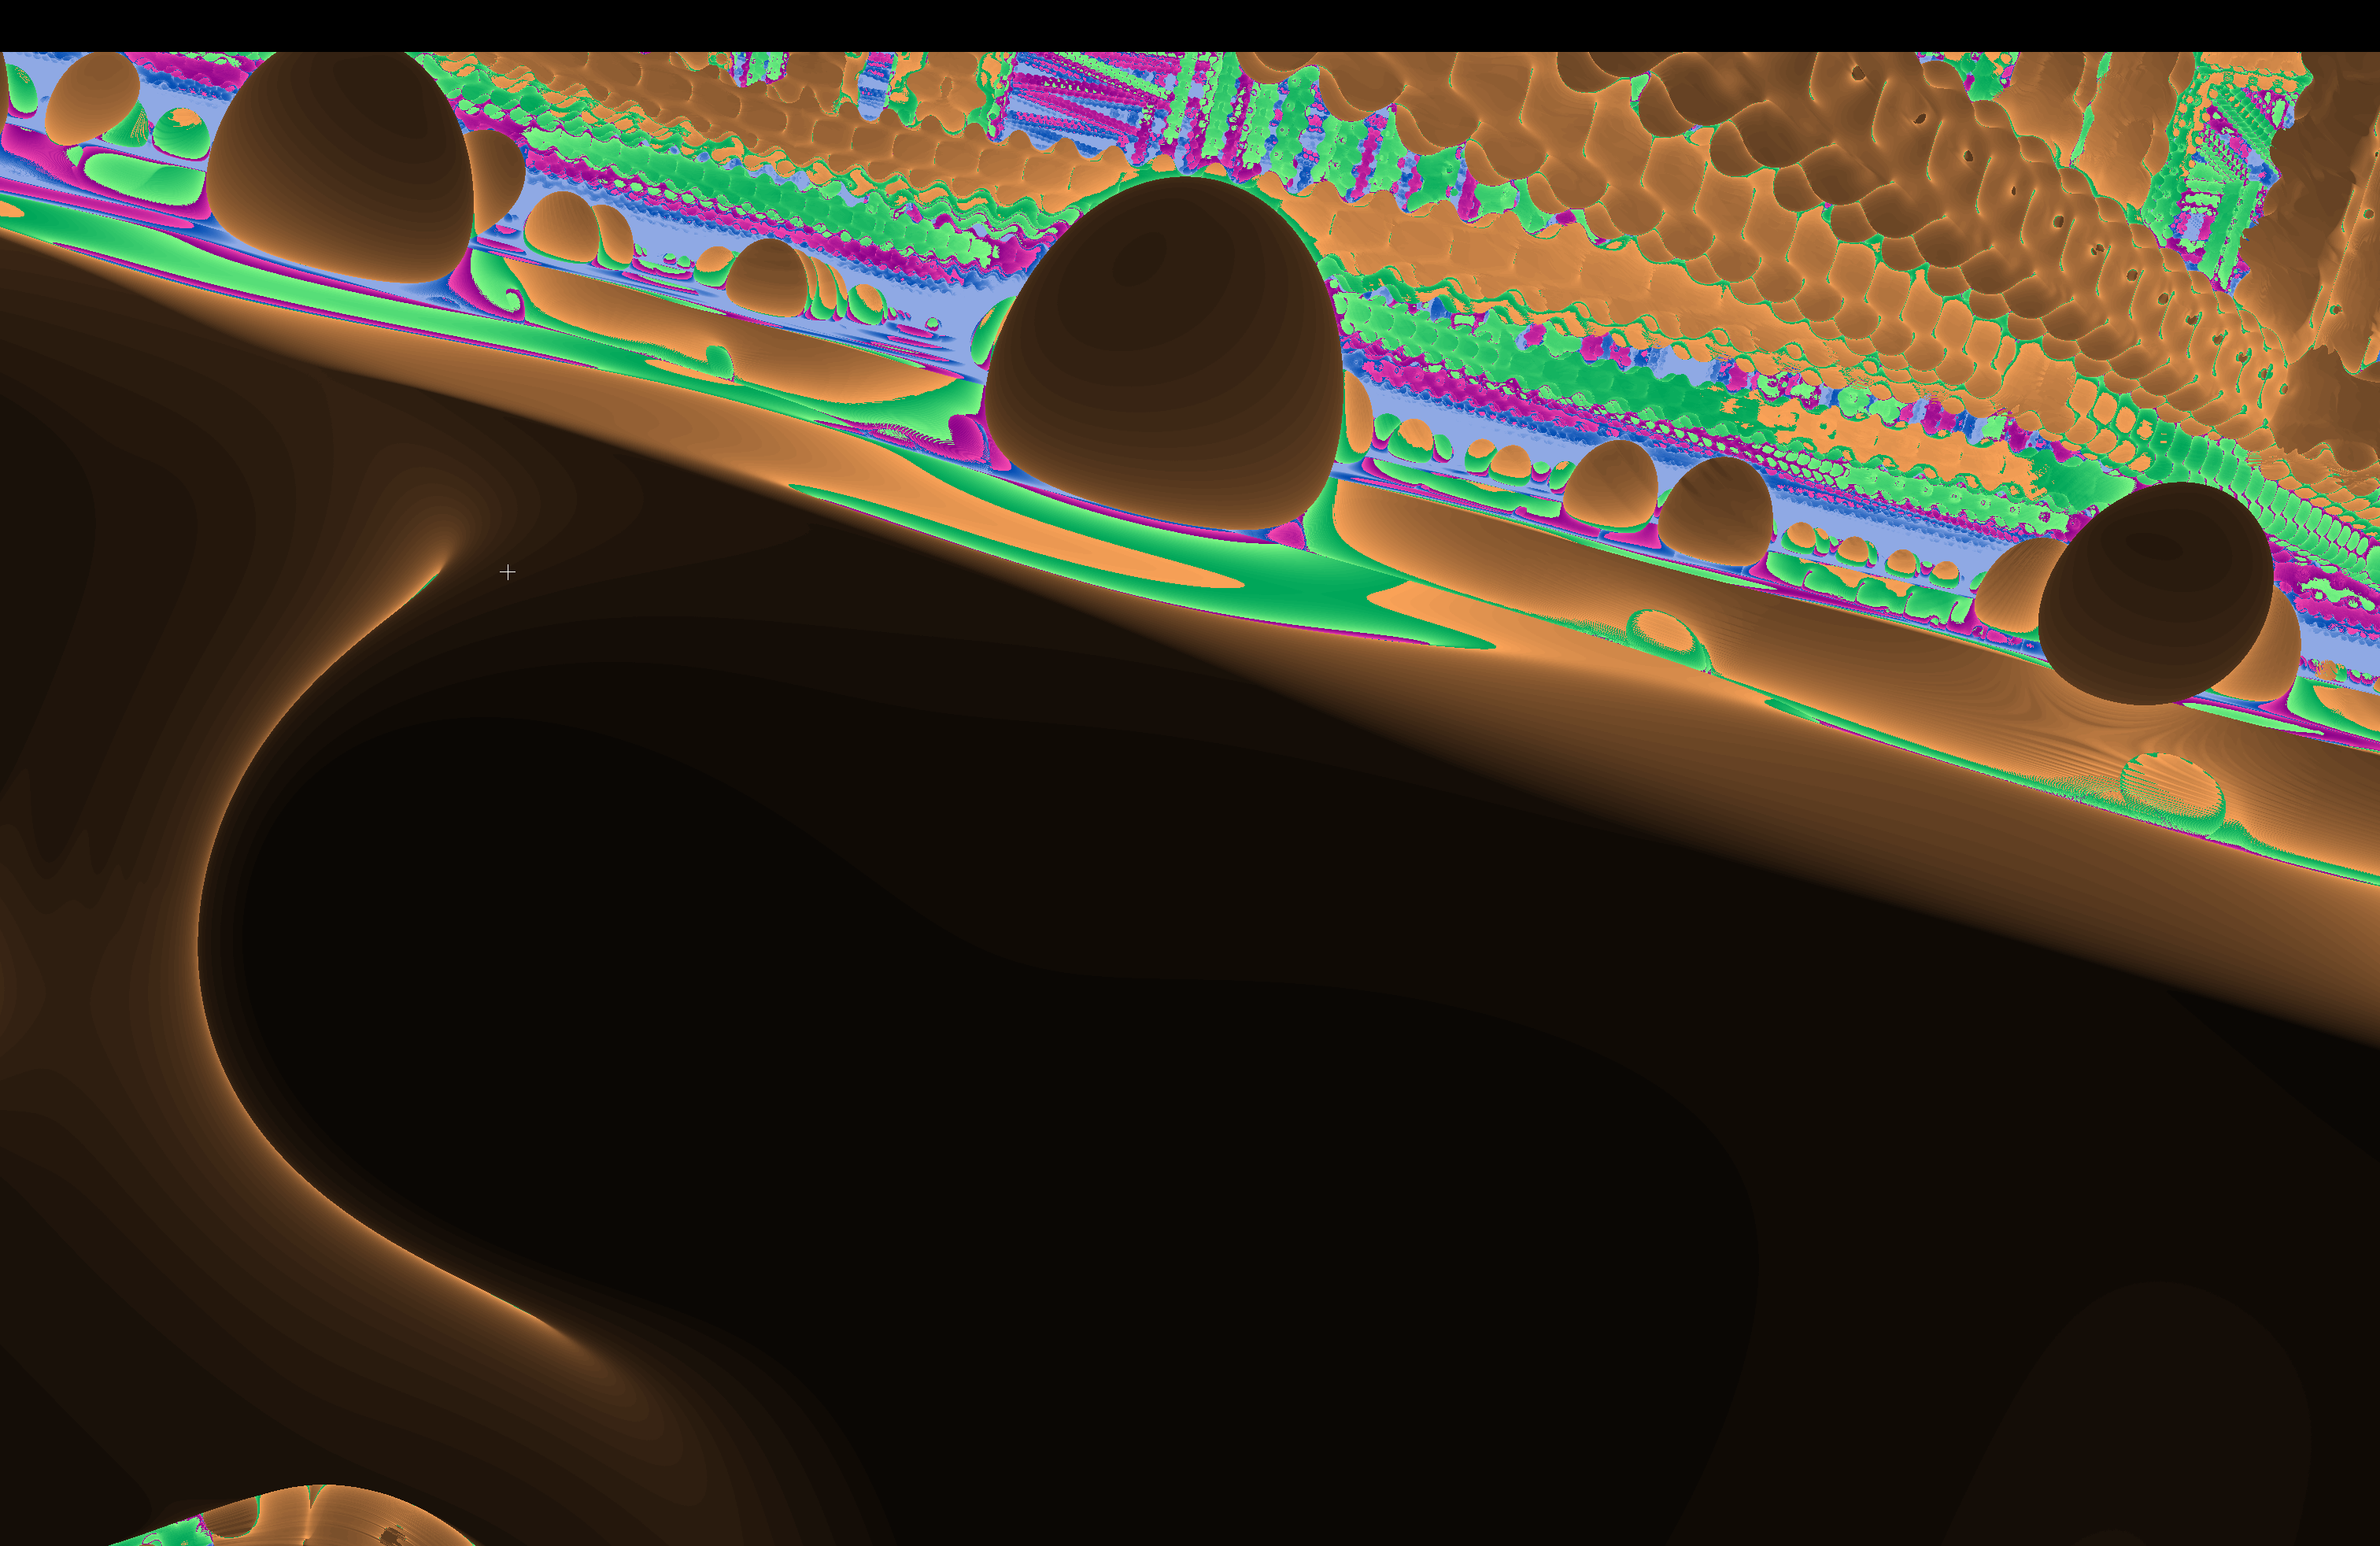
\includegraphics[width=\textwidth,height=0.28\textheight,keepaspectratio]{imgs/AppendixA/render_scaffold_glsl_edge.png}
    \caption{GLSL scaffold exterior edge. Large curved SDF boundary where the sphere-fold meets the scaffold lattice surface.}
\end{subfigure}\hfill
\begin{subfigure}[b]{0.48\textwidth}
    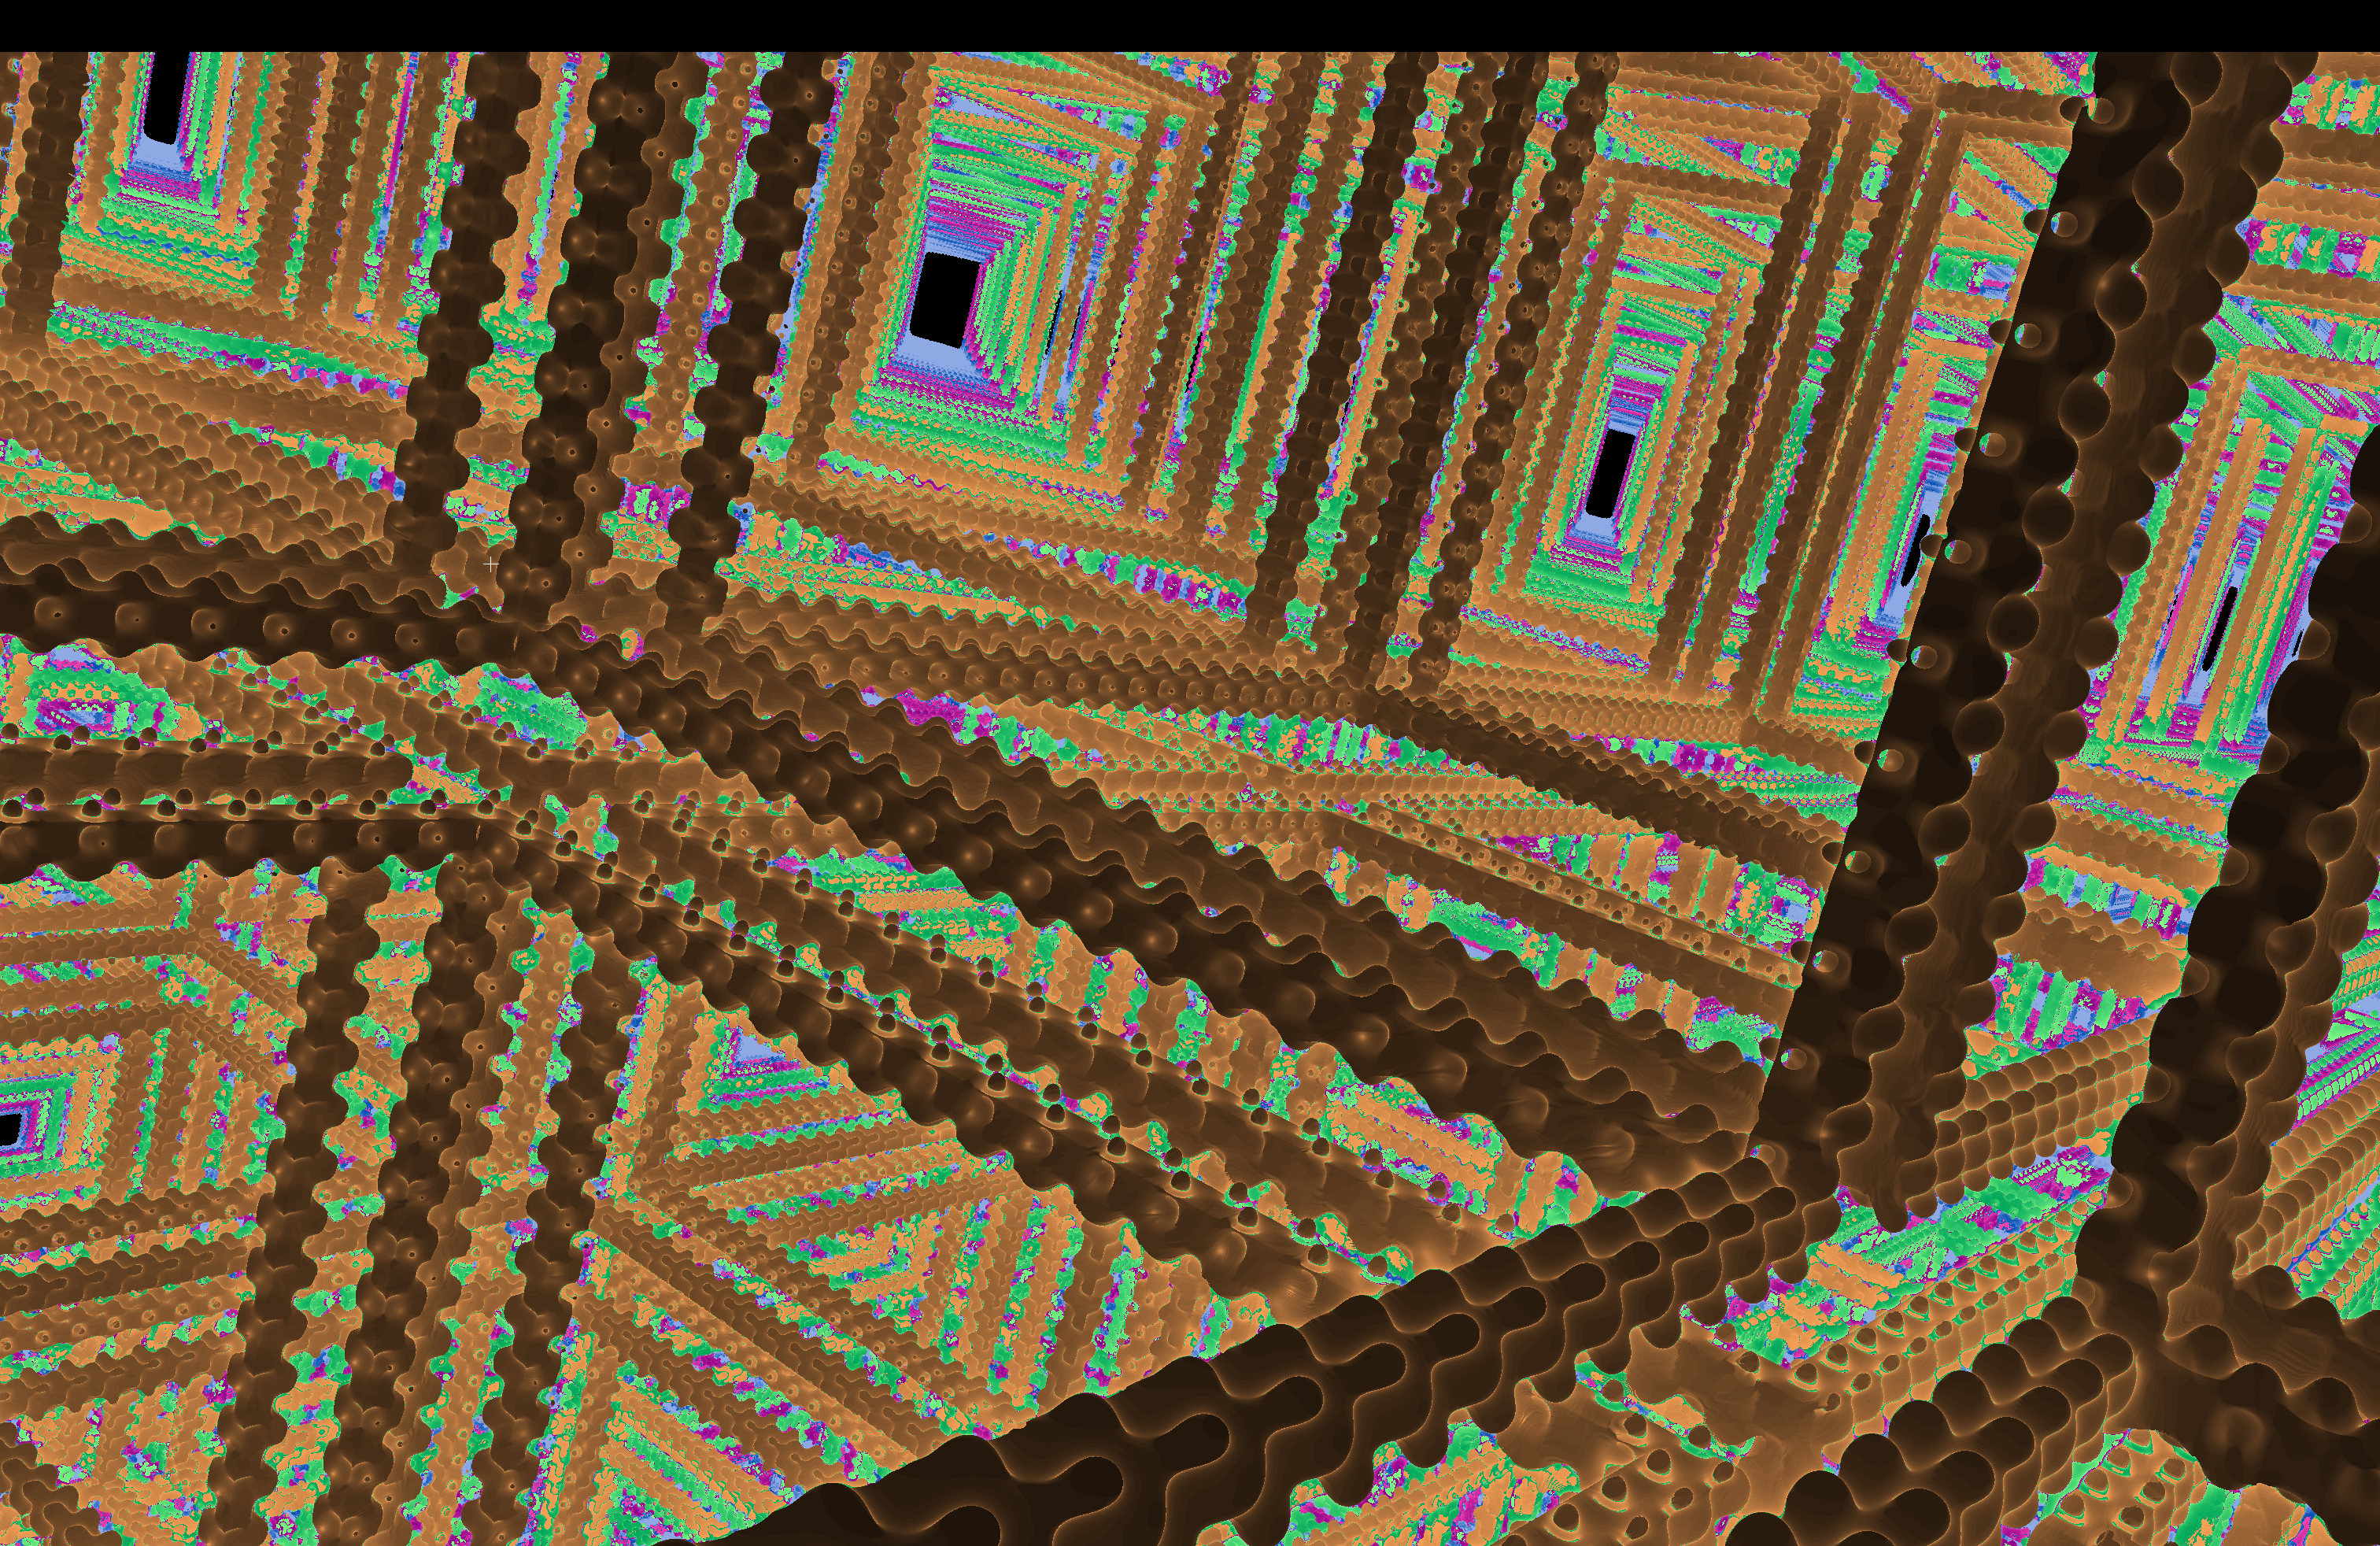
\includegraphics[width=\textwidth,height=0.28\textheight,keepaspectratio]{imgs/AppendixA/render_scaffold_glsl_corner.png}
    \caption{GLSL scaffold corner perspective. Deep lattice recession through frame diagonal; used to validate camera matrix.}
\end{subfigure}

\vfill

\begin{subfigure}[b]{0.48\textwidth}
    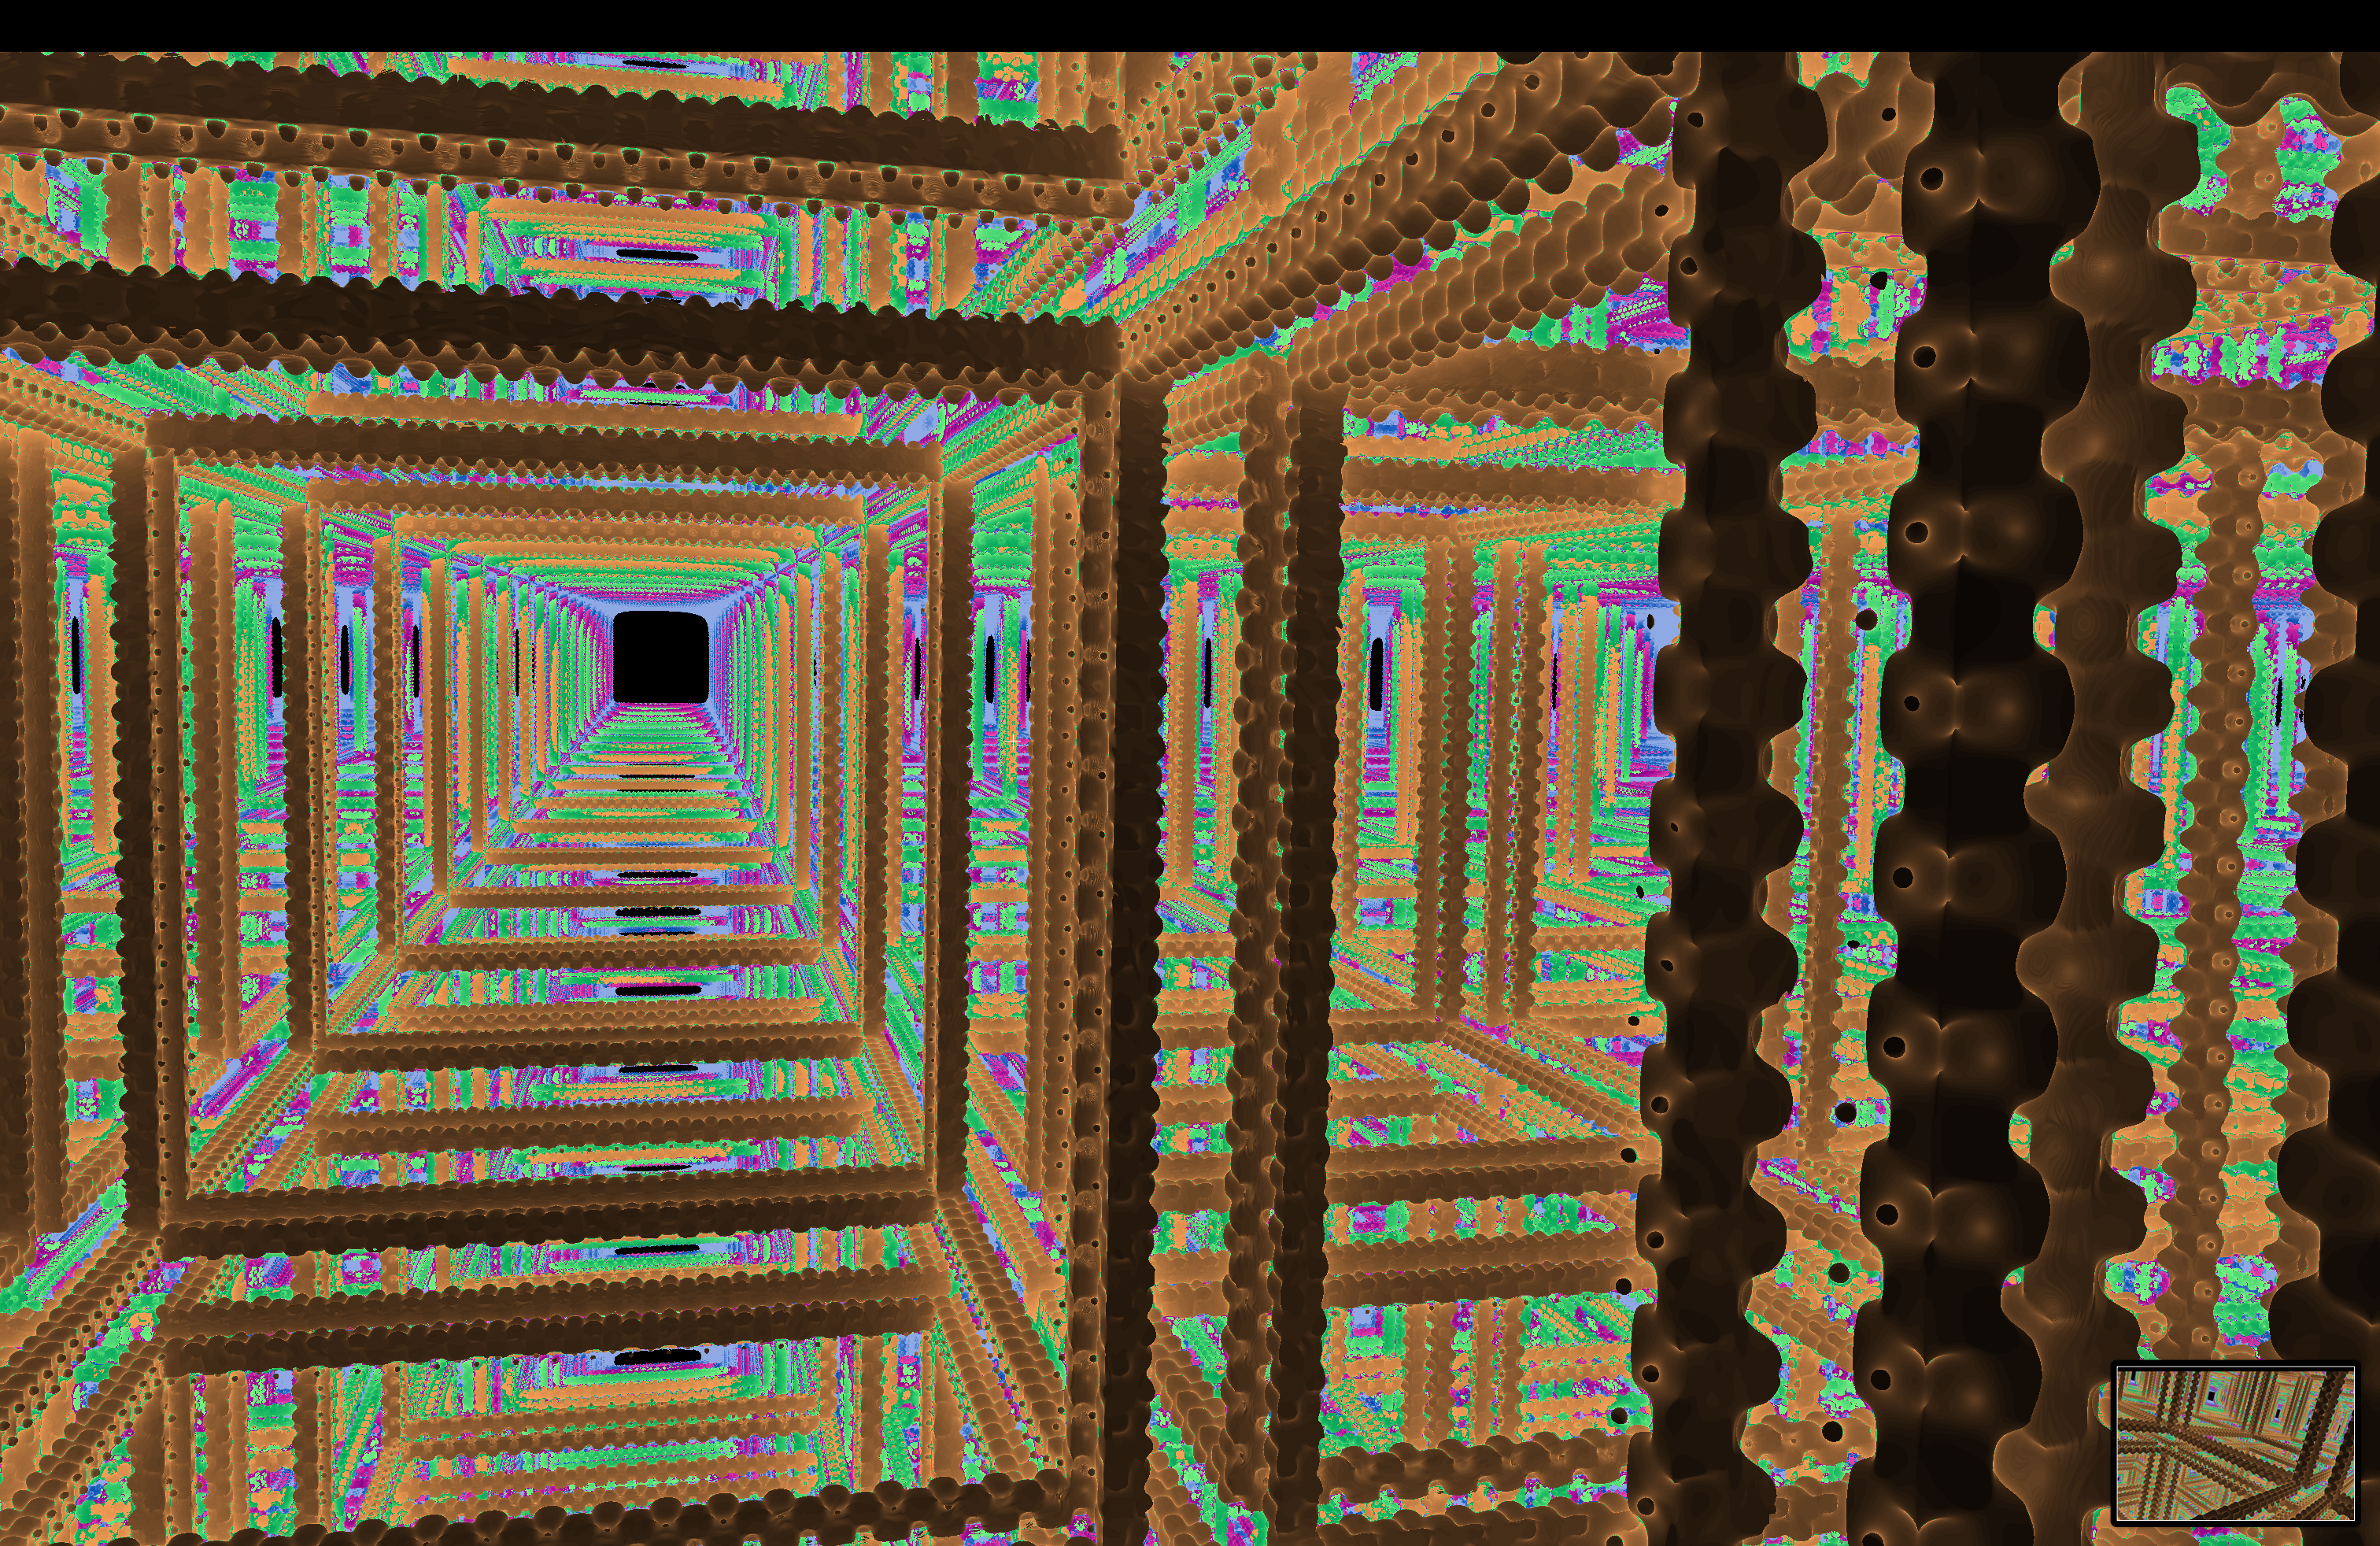
\includegraphics[width=\textwidth,height=0.28\textheight,keepaspectratio]{imgs/AppendixA/render_scaffold_glsl_tunnel.png}
    \caption{GLSL scaffold tunnel with twisted strut column on the right. Used as visual reference for RTL output comparison.}
\end{subfigure}\hfill
\begin{subfigure}[b]{0.48\textwidth}
    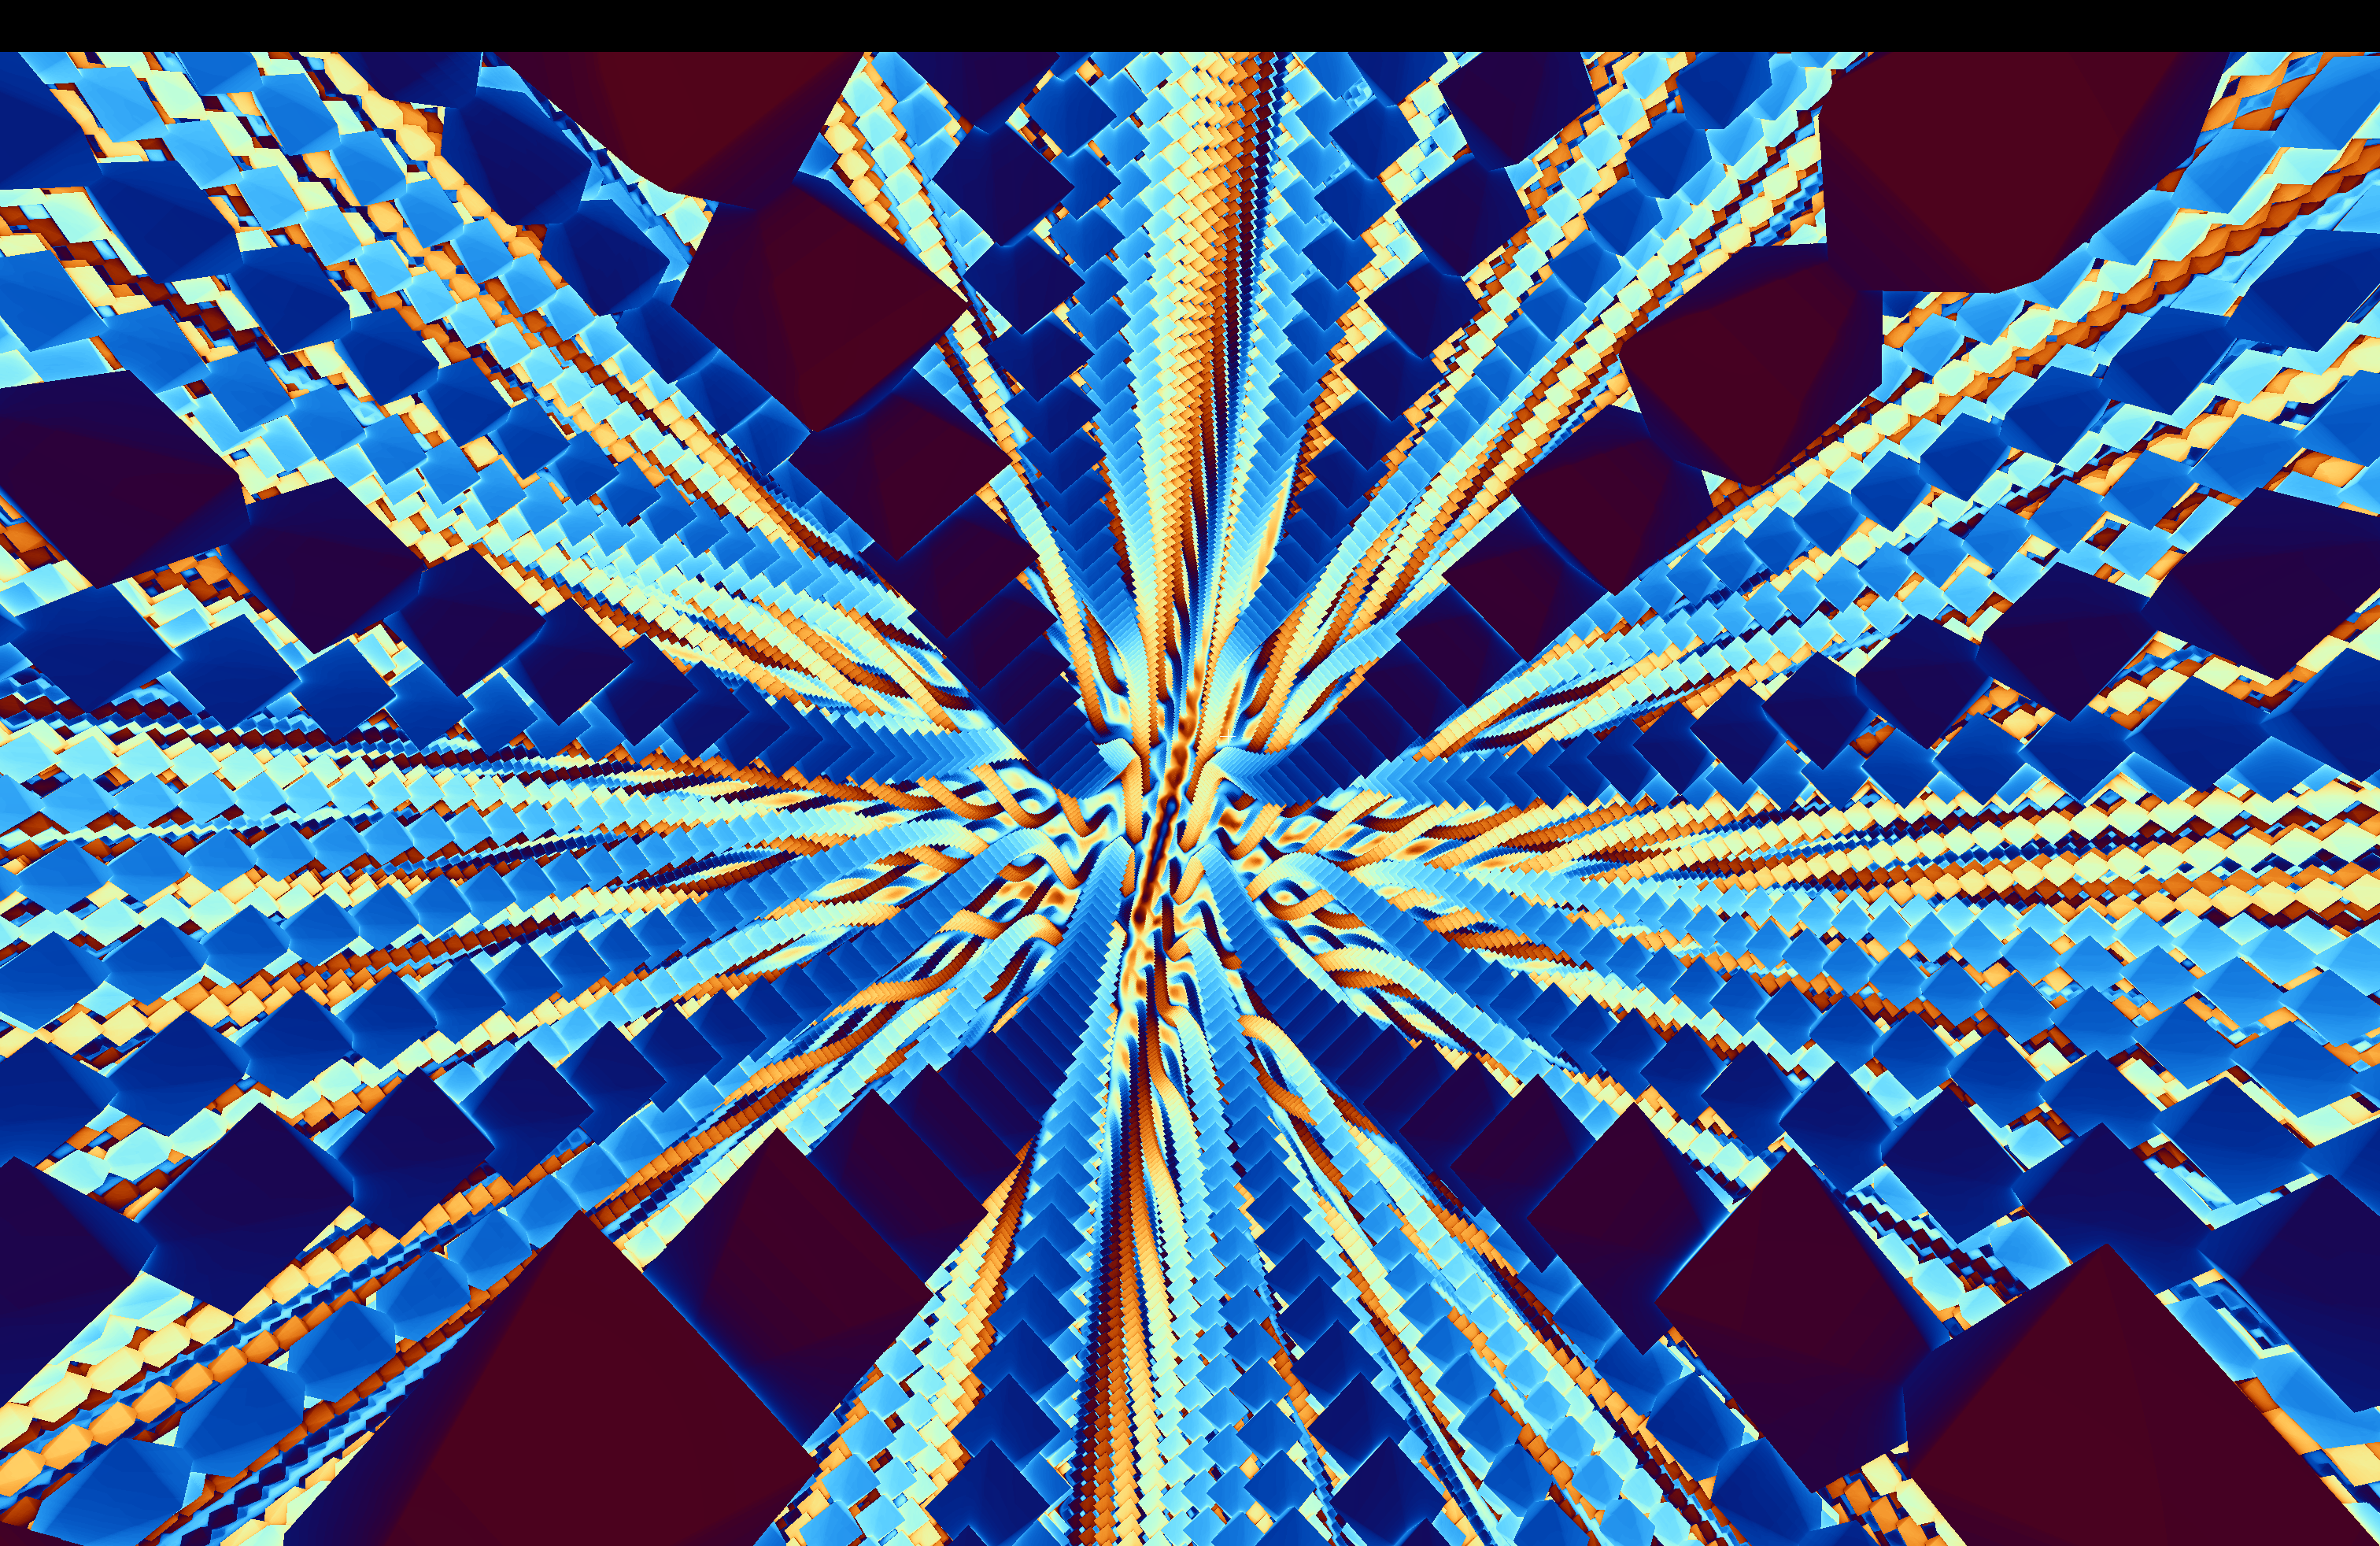
\includegraphics[width=\textwidth,height=0.28\textheight,keepaspectratio]{imgs/AppendixA/render_twisted_torus_glsl_centre.png}
    \caption{Twisted torus SDF in GLSL reference renderer, blue--orange palette, camera aimed at the twist convergence centre.}
\end{subfigure}
\caption{GLSL software reference renders, used for RTL visual verification and camera calibration.}
\end{figure}

\clearpage

% ----------------------------------------------------------------
%  Page 5 — Remaining GLSL renders + VR headset CAD gallery I
% ----------------------------------------------------------------
\begin{figure}[H]
\vspace*{-0.5cm}
\centering
\begin{subfigure}[b]{0.48\textwidth}
    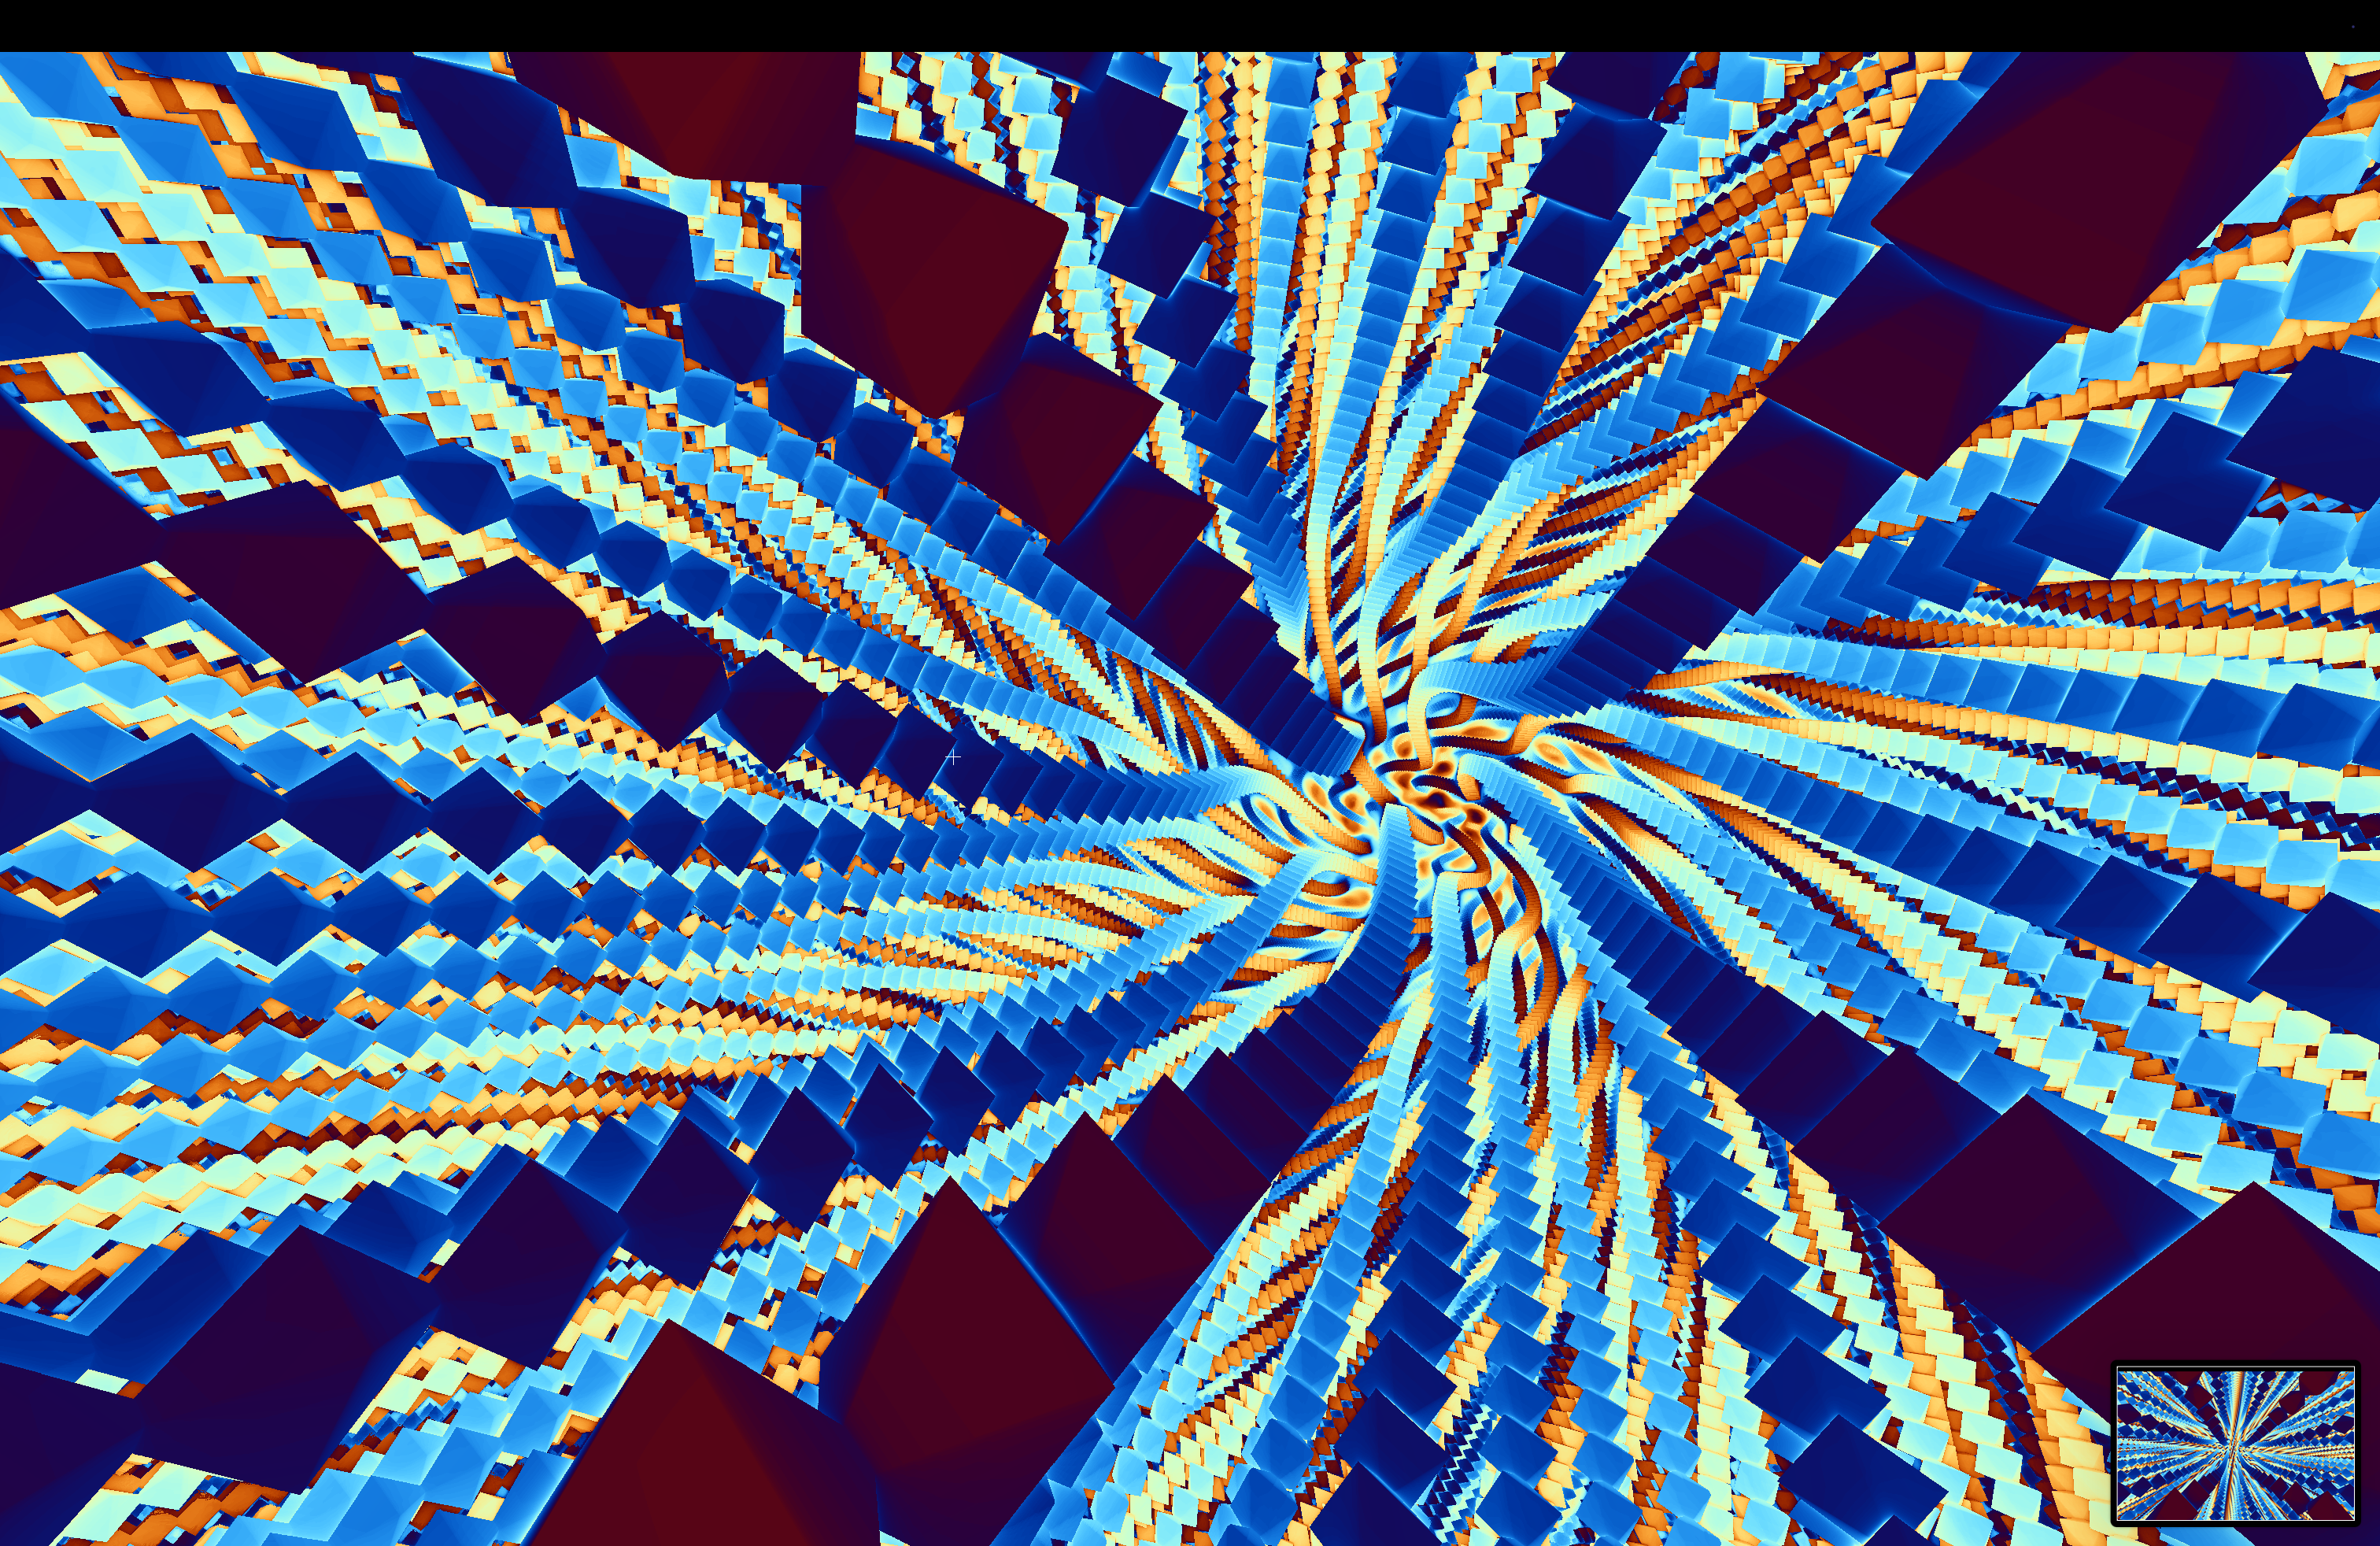
\includegraphics[width=\textwidth,height=0.28\textheight,keepaspectratio]{imgs/AppendixA/render_twisted_torus_glsl_spiral.png}
    \caption{Twisted torus spiral close-up. The twist parameter rotates the torus cross-section continuously around its axis.}
\end{subfigure}\hfill
\begin{subfigure}[b]{0.48\textwidth}
    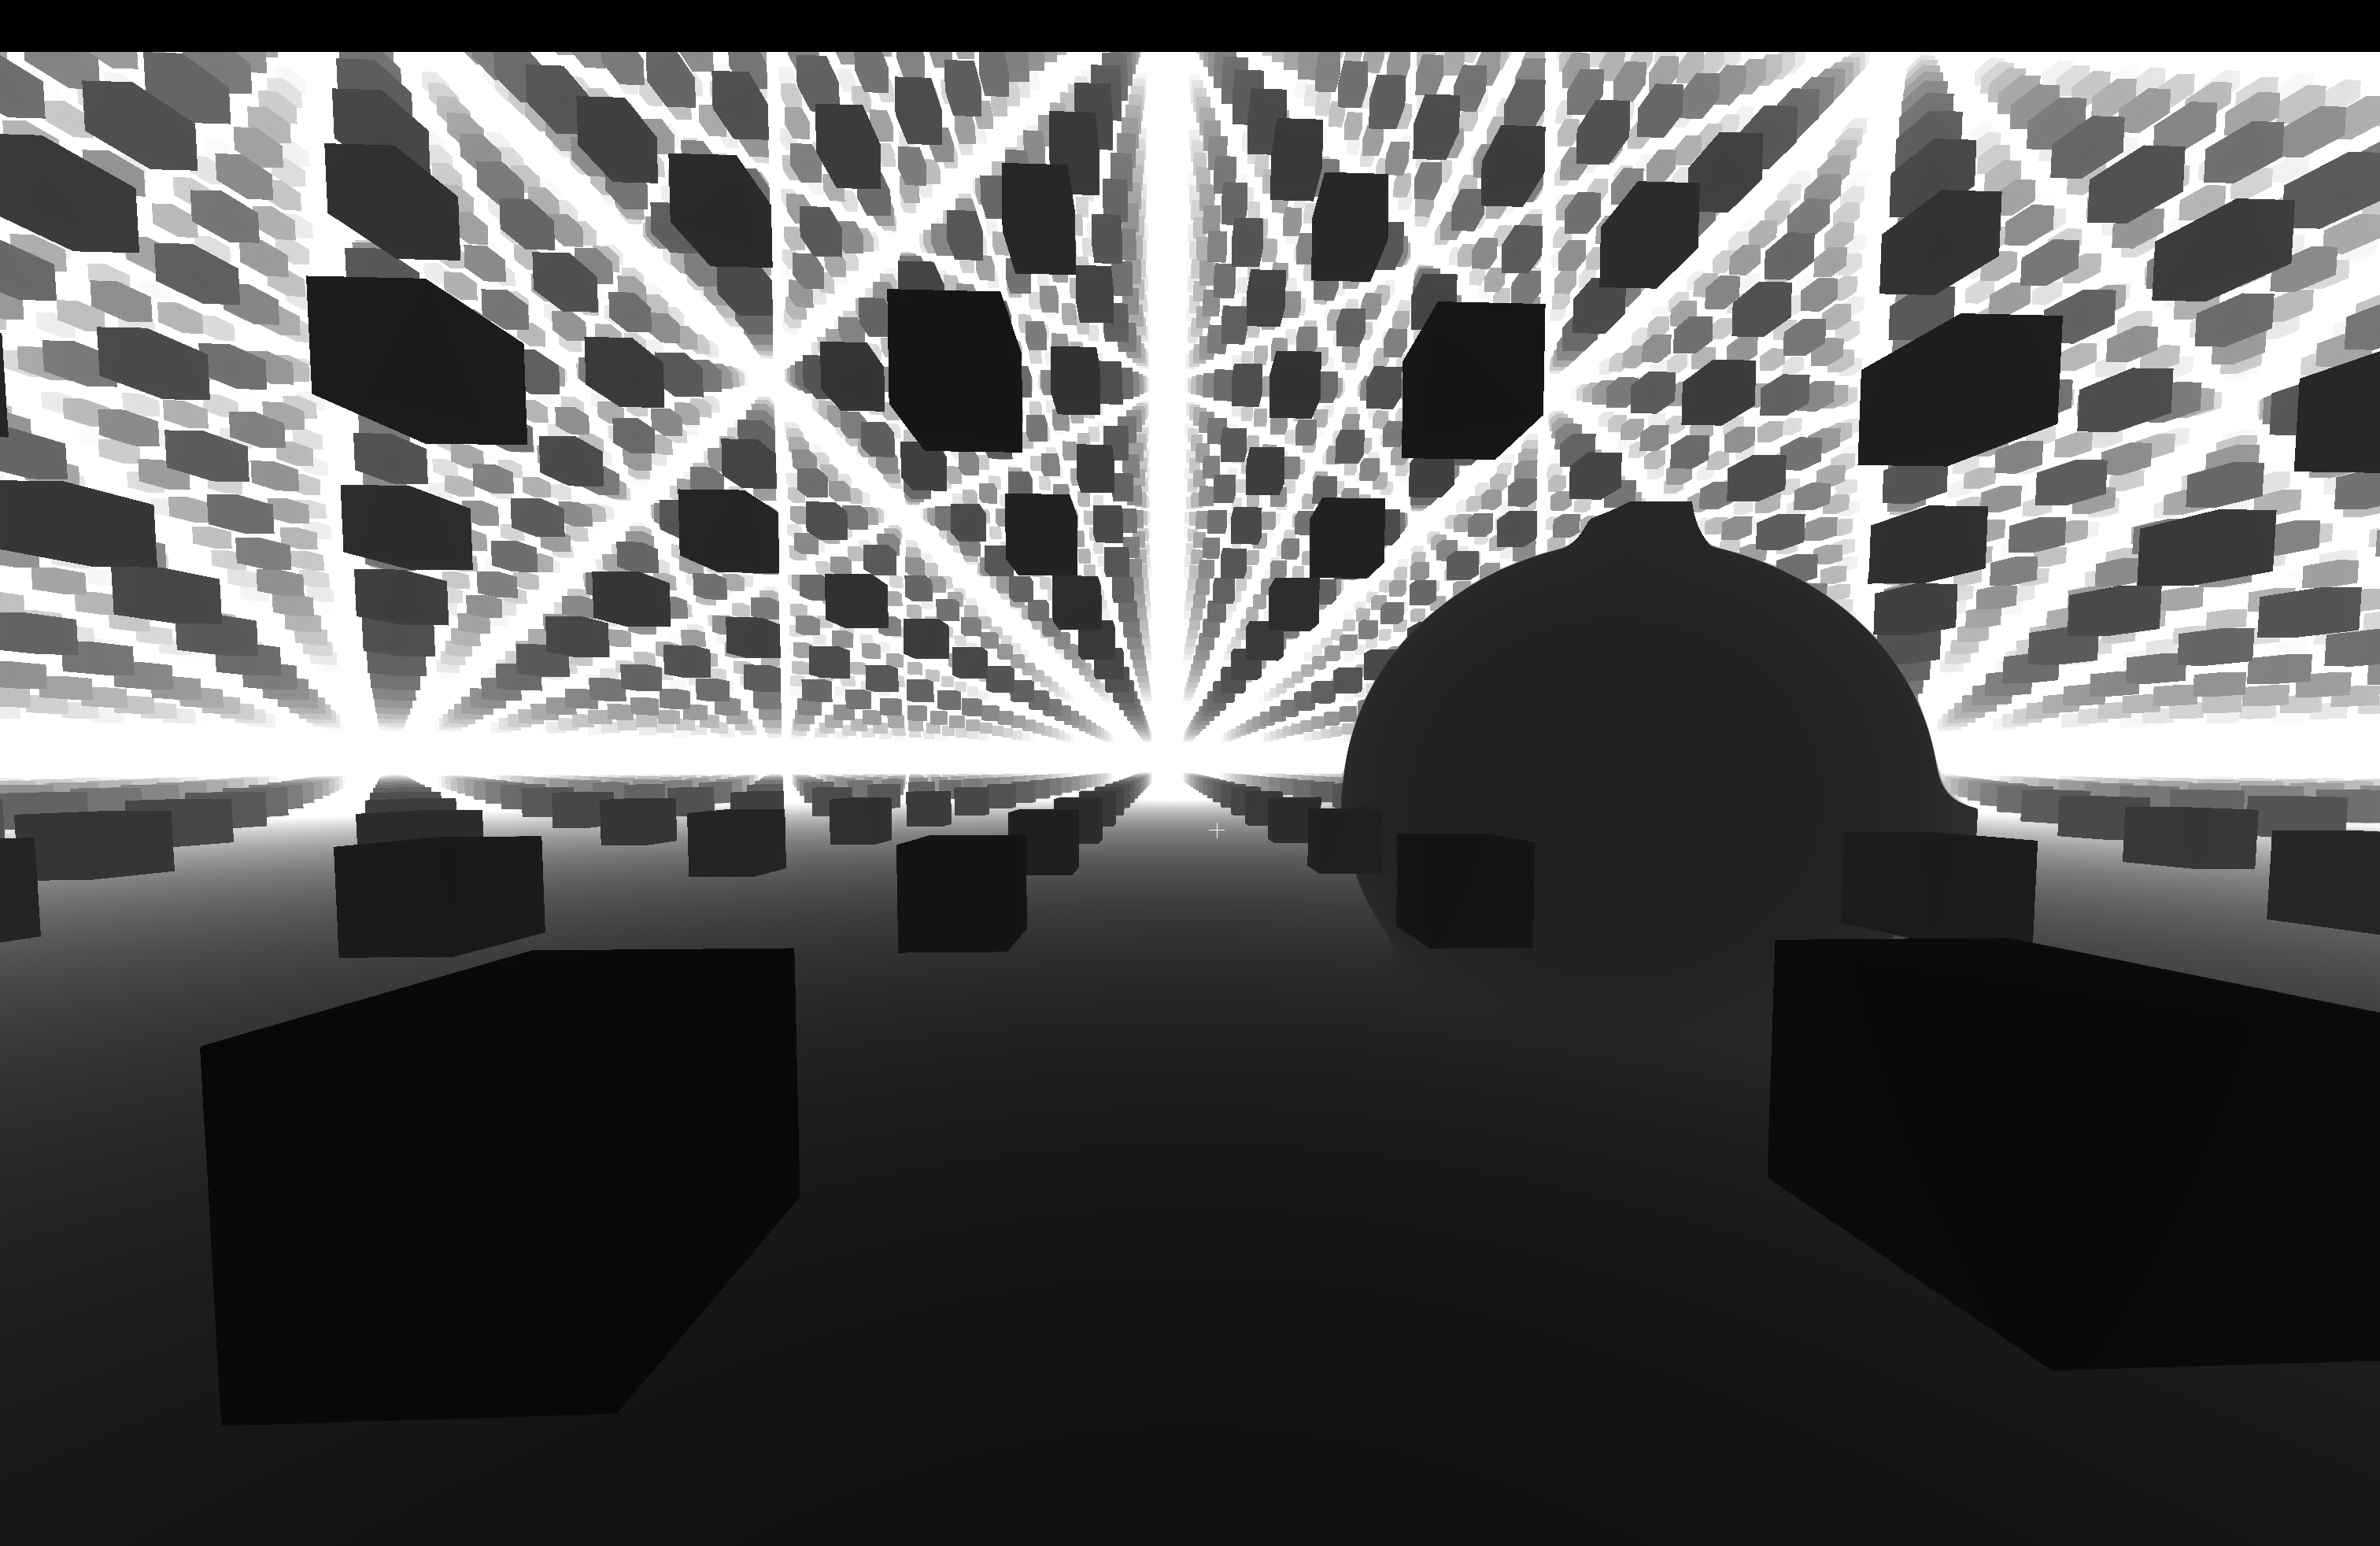
\includegraphics[width=\textwidth,height=0.28\textheight,keepaspectratio]{imgs/AppendixA/render_glsl_boxes_reference.png}
    \caption{GLSL reference scene, black-and-white box primitives on a reflective floor with starburst diffraction pattern.}
\end{subfigure}

\vfill

\begin{subfigure}[b]{0.48\textwidth}
    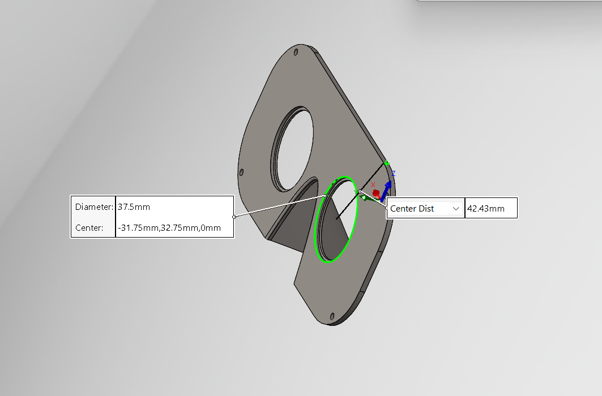
\includegraphics[width=\textwidth,height=0.28\textheight,keepaspectratio]{imgs/Headset_Images/lens_mount.png}
    \caption{Lens cup friction-fit CAD. 37\,mm biconvex lens diameter toleranced to $+0.5$\,mm for tool-free insertion.}
\end{subfigure}\hfill
\begin{subfigure}[b]{0.48\textwidth}
    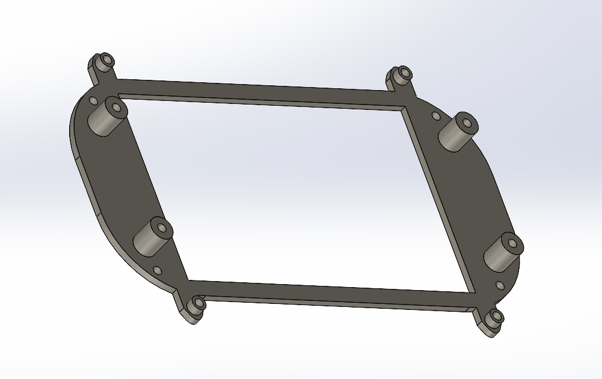
\includegraphics[width=\textwidth,height=0.28\textheight,keepaspectratio]{imgs/Headset_Images/screen_panel.png}
    \caption{Screen panel redesign. Entire panel rebuilt from scratch to achieve exact 45\,mm focal length for the 5-inch LCD.}
\end{subfigure}

\vfill

\begin{subfigure}[b]{0.48\textwidth}
    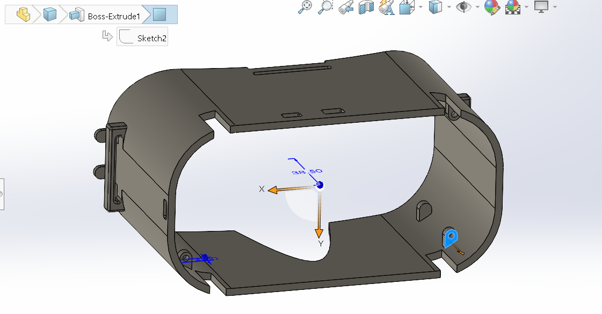
\includegraphics[width=\textwidth,height=0.28\textheight,keepaspectratio]{imgs/Headset_Images/body.png}
    \caption{Headset chassis body after focal-length depth adjustments. Extended body accommodates FPGA housing at the front.}
\end{subfigure}\hfill
\begin{subfigure}[b]{0.48\textwidth}
    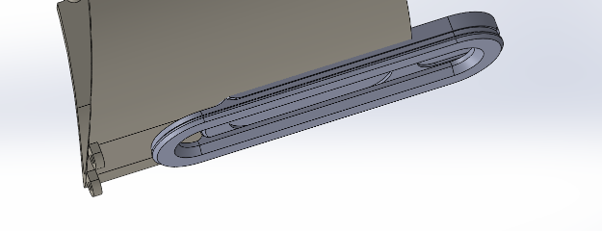
\includegraphics[width=\textwidth,height=0.28\textheight,keepaspectratio]{imgs/Headset_Images/quest2_strap_1.png}
    \caption{Quest~2 headstrap adapter arm, first image. Original velcro slot removed; adapter mated forward to clear screw holes.}
\end{subfigure}
\caption{GLSL reference renders continued and VR headset CAD gallery I.}
\end{figure}

\clearpage

% ----------------------------------------------------------------
%  Page 6 — VR headset CAD gallery II + system diagrams
% ----------------------------------------------------------------
\begin{figure}[H]
\vspace*{-0.5cm}
\centering
\begin{subfigure}[b]{0.48\textwidth}
    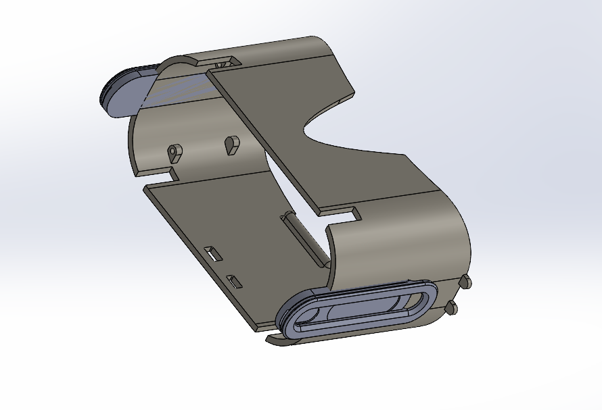
\includegraphics[width=\textwidth,height=0.28\textheight,keepaspectratio]{imgs/Headset_Images/quest2_strap_2.png}
    \caption{Quest~2 headstrap adapter arm, second image. Quest~3 geometry removed; Quest~2 clip mated directly to body.}
\end{subfigure}\hfill
\begin{subfigure}[b]{0.48\textwidth}
    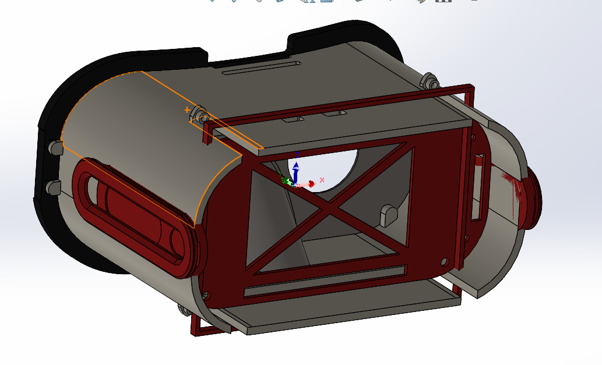
\includegraphics[width=\textwidth,height=0.28\textheight,keepaspectratio]{imgs/Headset_Images/fpga_housing_1.png}
    \caption{FPGA housing cavity. Internal dimensions set at $+0.5$--$1$\,mm tolerance for a tool-free friction fit of the PYNQ case.}
\end{subfigure}

\vfill

\begin{subfigure}[b]{0.48\textwidth}
    
\includegraphics[width=\textwidth,height=0.28\textheight,keepaspectratio]{imgs/Headset_Images/most_front_panel.png}
    \caption{Front panel with IMU mounting bracket and 4\,mm standoffs ensuring the MPU-6050 sits level for accurate tracking.}
\end{subfigure}\hfill
\begin{subfigure}[b]{0.48\textwidth}
    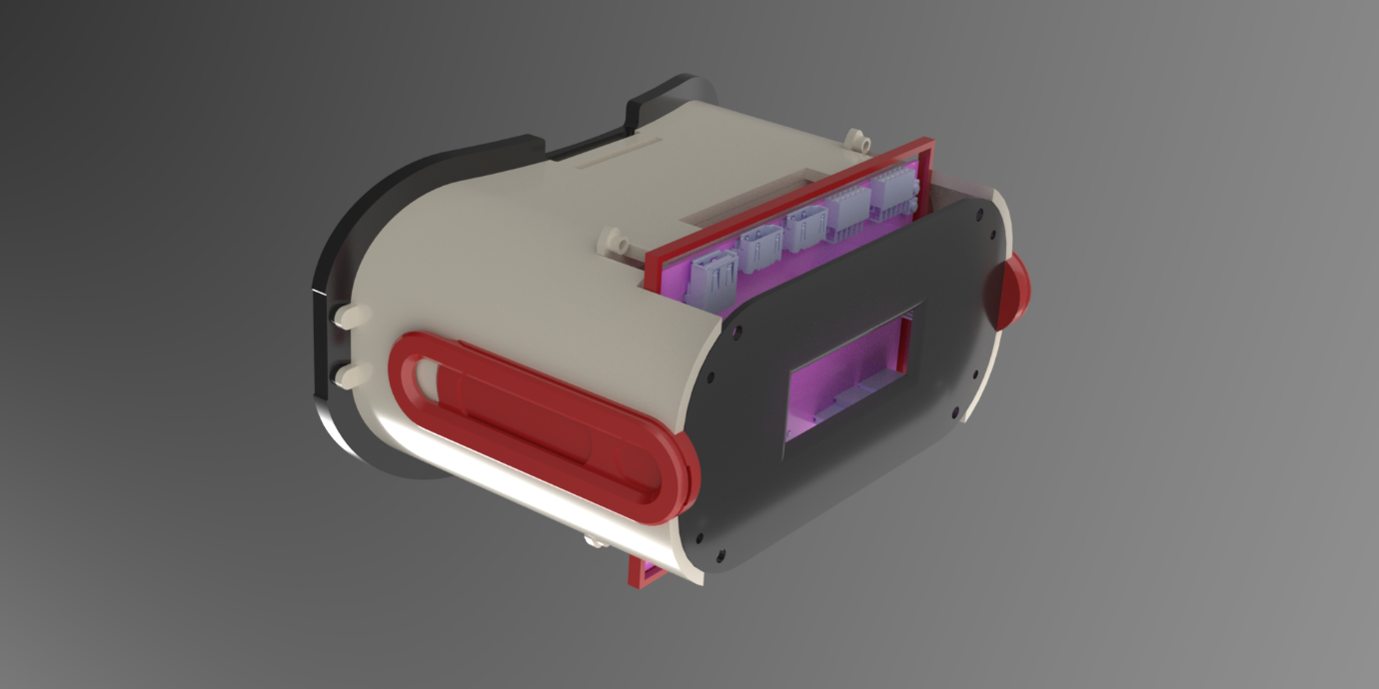
\includegraphics[width=\textwidth,height=0.28\textheight,keepaspectratio]{imgs/Headset_Images/final_rendered.png}
    \caption{Final SolidWorks Visualize render of the complete headset assembly prior to 3D printing.}
\end{subfigure}

\vfill

\begin{subfigure}[b]{0.48\textwidth}
    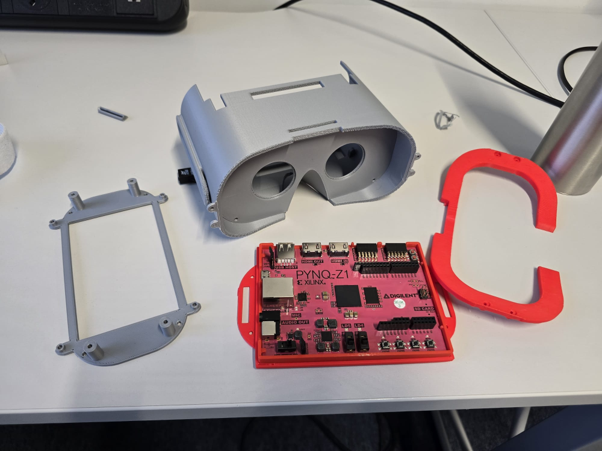
\includegraphics[width=\textwidth,height=0.28\textheight,keepaspectratio]{imgs/Headset_Images/physical_construction.png}
    \caption{Physical construction phase. Parts printed and assembled; minor redesigns for HDMI cable clearance performed here.}
\end{subfigure}\hfill
\begin{subfigure}[b]{0.48\textwidth}
    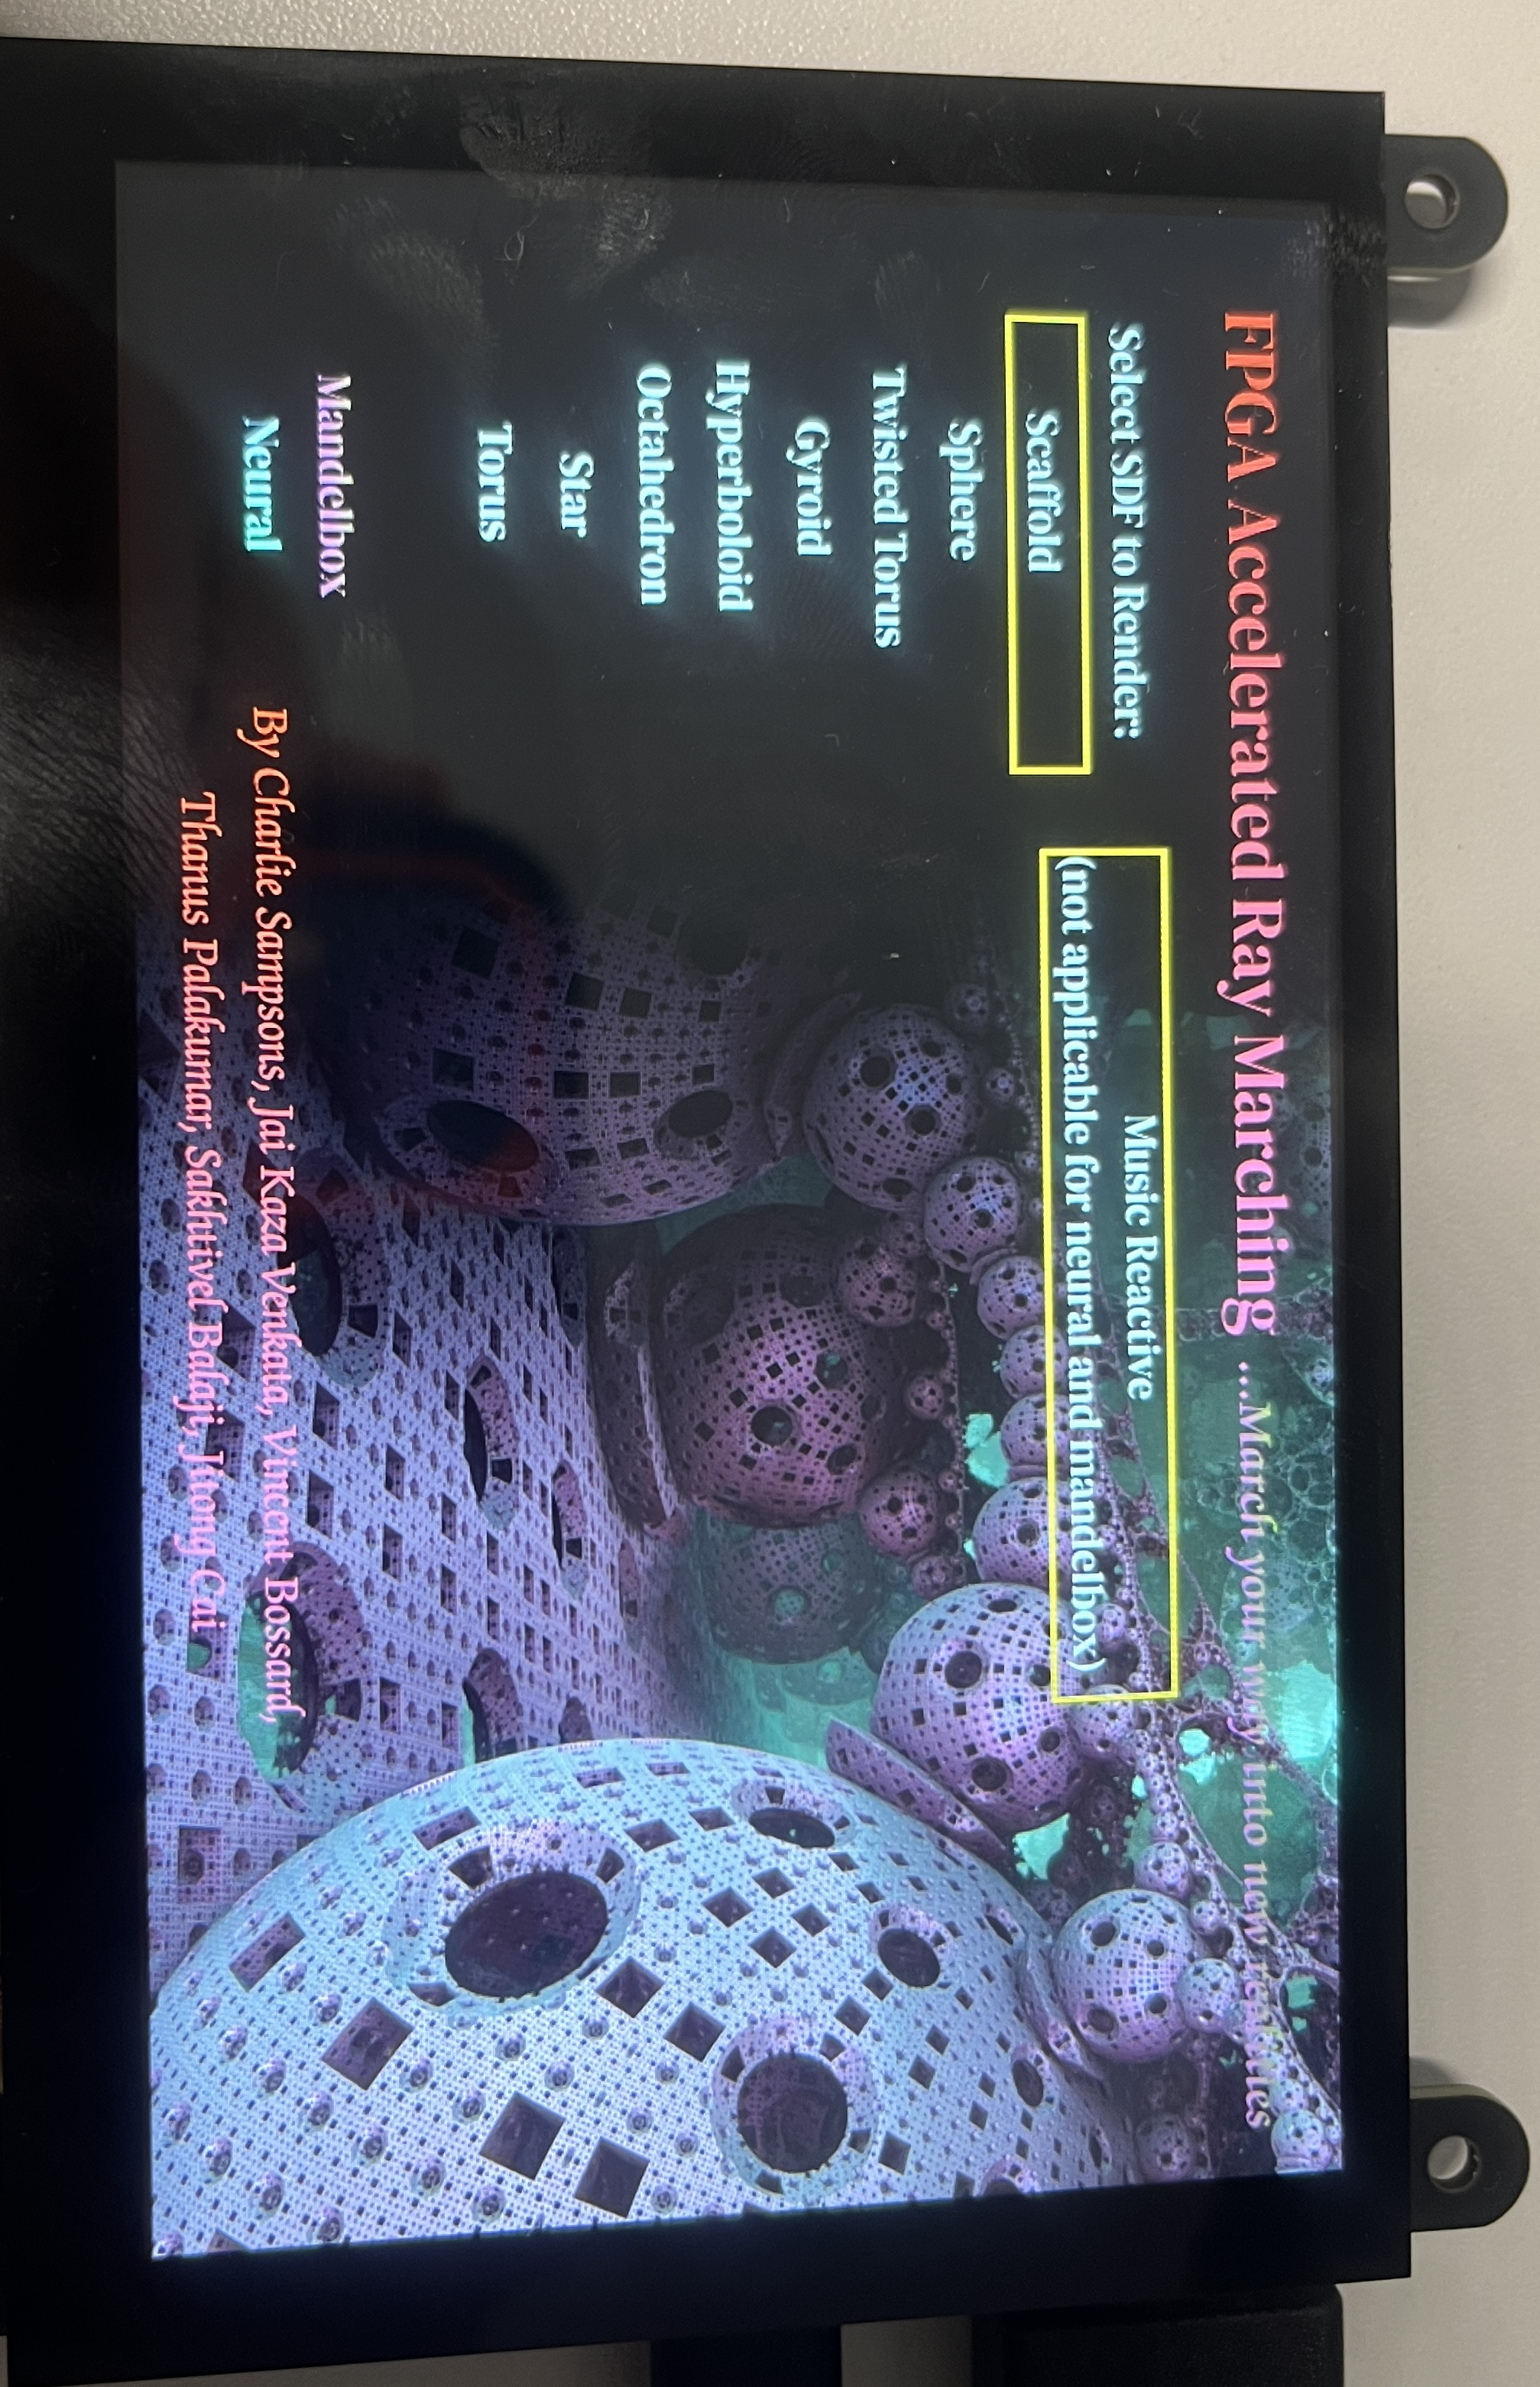
\includegraphics[width=\textwidth,height=0.28\textheight,keepaspectratio]{imgs/ui_no_shift.jpg}
    \caption{Stable scene-selector UI on HDMI output. No frame shift after FCLK0 drop sequence introduced during bitstream swap.}
\end{subfigure}
\caption{VR headset CAD gallery II and system UI --- final design, physical build, and stable display output.}
\end{figure}
